% -*- latex -*- This is a LaTeX document.
% $Id: phd-thesis.tex,v 1.57 2007-05-23 21:19:08 cananian Exp $
%%%%%%%%%%%%%%%%%%%%%%%%%%%%%%%%%%%%%%%%%%%%%%%%%%%%%%%%
\documentclass[letterpaper,draftnotice]{phd-thesis}
\usepackage{verbatim}
\usepackage{alltt}
\usepackage{epigraph}
\usepackage{makeidx}
\usepackage[square,sort&compress,numbers]{natbib}
\usepackage[pdfusetitle,pagebackref,colorlinks,bookmarks,bookmarksnumbered,pdfpagelayout=TwoPageRight,breaklinks]{hyperref} % ooh, hyperlinks!
%\hypersetup[linktocpage] % useful when previewing with dvi
\usepackage{hypernat}
\usepackage{bold-extra}
%\makeindex % punting!

% draft options:
%\usepackage[light,first,bottomafter,timestamp]{draftcopy}
%\usepackage{showidx}
%\draftcopyName{DRAFT $Revision: 1.57 $}{70}

\notesfalse % comment out this line to turn on notes.

% nicer bibliography back-references.
\renewcommand*{\backref}[1]{} % tell backref we're using the alt interface
\renewcommand*{\backrefalt}[4]{%
  % alternative interface
  % #1: number of distinct back references
  % #2: backref list with distinct entries
  % #3: number of back references including duplicates
  % #4: backref list including duplicates
  [on
  \ifnum#1=1 %
    p.~%
  \else%
    pp.~%
  \fi%
  #2.]
}
% describe these back-references; also add the bibliography to the toc.
\renewcommand{\bibsection}{\chapter{Bibliography}}
\newcommand{\bibpreamble}{%
Each citation is followed by a bracketed list of the pages
on which it appears.\\
DOI names can be resolved at \url{http://doi.org}.
}

% hyperlink doi references
\newcommand{\doi}[1]{doi: \href{http://hdl.handle.net/#1}{\urlstyle{rm}\nolinkurl{#1}}}

\author{C.~Scott~Ananian}
\newcommand{\subtitle}{Architectural and Compiler Support for Strongly
                       Atomic Transactional Memory}
\newcommand{\subdate}{May 21, 2007}
\title{\subtitle}
\date{\subdate}

% definitions for this thesis
\newcommand{\atomic}{\texttt{atomic}\xspace}
\newcommand{\funcname}[1]{\ensuremath{\text{\sc #1}}}
\newcommand{\var}[1]{\ensuremath{\text{\it #1}}}
\newcommand{\fref}[2]{\ensuremath{#1\text{\tt .#2}}}
\newcommand{\addr}[1]{\ensuremath{\text{\tt \&}(#1)}}
\newcommand{\tuple}[1]{\ensuremath{\left\langle #1 \right\rangle}}
\newcommand{\FLAG}{\texttt{FLAG}\xspace}
\newcommand{\Spin}{\textsc{Spin}\xspace}
\newcommand{\flex}{\textsc{Flex}\xspace}
\newcommand{\Flex}{\textsc{Flex}\xspace} % initial cap version
\newcommand{\apex}{\textsc{ApeX}\xspace}
\newcommand{\lapex}{\textsc{Large ApeX}\xspace}
\newcommand{\hyx}{\textsc{HyApeX}\xspace}
\newcommand{\naive}{naive\xspace} % Charles doesn't like the \"\i version
\newcommand{\etal}{\textit{et al.}\@\xspace}

\newcommand{\contribution}[1]{\begin{quote}\textbf{\textsf{#1}}\end{quote}}

\begin{document}
\bibliographystyle{plainnat}
%\frontmatter
\newcommand{\nl}{\\[0.5\baselineskip]}
\newcommand{\tight}{\\[-0.2\baselineskip]}
\begin{titlepage}
%\vspace*{0.5cm}
\begin{center}
\textbf{\LARGE \subtitle}\\
{\large by}\\
{\large C. Scott Ananian}\nl
M.Sc Electrical Engineering and Computer Science,\\
Massachusetts Institute of Technology, 1999;\\
B.S.E. Electrical Engineering,\\
Princeton University, 1997.
\end{center}
Submitted to the Department of Electrical Engineering and Computer Science
in partial fulfillment of the requirements for the degree of
Doctor of Science in Electrical Engineering and Computer Science
at the Massachusetts Institute of Technology.
\begin{center}
\subdate\nl
Copyright 2005 Massachusetts Institute of Technology\\
All right reserved.
\end{center}

\vspace{0.5cm}
\begin{flushright}
Author\hrulefill\tight
\hfill Department of Electrical Engineering and Computer Science\tight
\hfill \subdate\nl
Certified by\hrulefill\tight
\hfill Martin Rinard\tight
\hfill Thesis Supervisor\nl
Accepted by\hrulefill\\
\hfill Arthur C. Smith\tight
\hfill Chairman, Department Committee on Graduate Theses\nl
\end{flushright}
\end{titlepage}\setcounter{page}{2}
{% abstract page
\begin{center}
\subtitle\tight
by\tight
C. Scott Ananian\nl
Submitted to the\tight
Department of Electrical Engineering and Computer Science\nl
\subdate\nl
\end{center}

\begin{flushleft}
In partial fulfillment of the requirements for the Degree of Doctor of
Science in Electrical Engineering and Computer Science.
\end{flushleft}

\vspace{0.75cm}
\centerline{\LARGE\textbf{Abstract}}
\vspace{0.3cm}

%% This is the abstract of my thesis.

Transactions map naturally to human intuition of atomic action in
concurrent systems, eliminating the necessity of locking discipline.
This thesis presents efficient implementations of transactions for
three platforms: an object-oriented software-only system, a scalable
system using a custom processor extension, and in a hybrid of the two
systems, obtaining the benefits of both.  I also present formal models
of the implementation which have been mechanically checked for correct
behavior.

I also explore the implications of available, efficient, and usable
transactions on high-level language design, presenting solutions for
transaction nesting, merging, and loophole mechanisms.  This presents
a solution to the vexing ``I/O'' and modularity problems with
existing transactional mechanisms.  I also present compiler analyses
and type systems to further improve the efficiency, safety, and
usability of our transaction mechanisms.


\vspace{0.5cm}
\begin{flushleft}
Thesis Supervisor: Martin Rinard\\
Title: Professor, Laboratory for Computer Science\\
\end{flushleft}
}
\tableofcontents\listoffigures\listoftables\listofalgorithms


%\mainmatter
%\chapter{Introduction}
%\section{Locking vs nonblocking synchronization}
%\section{Transactions and transactional memory}
\index{Lock(s)!problems with}
Atomicity in shared-memory multiprocessors is 
conventionally provided
via mutual-exclusion \defn{locks} (see, for example,
\cite{Tanenbaum92}[p.~35]).  Although locks are easy to
implement using test-and-set, compare-and-swap, or
load-linked/{\bp}store-conditional instructions, they introduce a host of
difficulties.  Protocols to avoid deadlock when locking multiple
objects often involve acquiring the locks in a consistent linear
order, which may make programming with locks error-prone and introduce
significant overheads.  The granularity of each lock must also be
explicitly chosen: locks which are too fine introduce unnecessary
space and time overhead, while locks which are too coarse sacrifice
attainable parallelism (or may even deadlock).  Every access to a
shared object must hold some lock protecting that object, regardless
of whether another thread is actually attempting to access the same object.

\defn{Transactions} are
an alternative means of providing concurrency control.
A transaction can be thought of as a sequence of loads and stores
performed as part of a program which either
\defn{commits} or \defn{aborts}.  If a transaction
commits, then all of the loads and stores appear to have run
atomically with respect to other transactions.  That is, the
transaction's operations are not interleaved with those of other
transactions.  If a transaction aborts, then none of its stores take
effect and the transaction may be restarted, with some mechanism to
ensure forward progress.

This thesis will provide efficient implementations of
transaction primitives to enable their general use.
By structuring concurrency at a high level with transactions, human
programmers no longer have to manage the details required to ensure
atomicity.  Programmers have difficulty correctly understanding the global
interactions between multiple threads, each holding its own set of
locks, and a full mental model of the global concurrency structure
must be kept in mind when writing synchronization code.
The simpler ``global atomicity'' guaranteed under the
transactional model eliminates errors and simplifies the conceptual
model of the system, making future modifications safer as
well.  Previously, implementations of transactions were too slow for
general use.

The transaction primitives presented in this thesis can exploit
optimistic concurrency, provide fault tolerance, and prevent delays by
using non-blocking synchronization.
Although transactions can be implemented using mutual exclusion
(locks), our algorithms will utilize non-blocking synchronization
\index{Non-blocking synchronization}\index{Synchronization!non-blocking}
\cite{Lamport77,Herlihy88,HerlihyLuMo03,MassalinPu91,GreenwaldCh96} to
exploit optimistic concurrency among transactions.  Non-blocking
synchronization offers a number of advantages; foremost for the
concerns of this thesis is fault tolerance.  A process that fails
while holding a lock within a critical region can prevent all other
non-failing processes from ever making progress.  It is in general not
possible to restore the locked data structures to a consistent state
after such a failure.  Non-blocking synchronization offers a graceful
solution to this trouble, as non-progress or failure of any one thread
will not affect the progress or consistency of other threads or the
system.

Implementing transactions using
non-blocking synchronization offers performance benefits as well.
When mutual exclusion is used to enforce atomicity, page
page faults, cache misses, context
switches, I/O, and other unpredictable events may result in delays to the
entire system. Non-blocking
synchronization allows undelayed processes or processors to continue
to make progress.
Similarly, in real-time systems, the use of non-blocking
synchronization can prevent \defnlti{Priority inversion}
\index{Lock(s)!priority inversion} in the system
\cite{Jones97}, although na\"{\i}ve implementations may result in
starvation of low-priority tasks (see \charef{progress} for a discussion).

In this thesis I will show how transactions can be integrated into an
object-oriented language and used for backtracking, exception
handling, and concurrency control in new programs, in addition to
expressing atomicity and fault-tolerance.

One of the common synchronization mistakes made in lock-based
object-oriented code is
the ``multiple object problem'': when lock A protects object A, and
lock B protects object B, it is easy to get into trouble when writing
routines which involve both objects A and B.  Either insufficient
locks are taken, or both locks are taken without carefully considering
deadlock, or else one object's locks are released and reacquired during the
operation allowing atomicity to be broken.
In \charef{safe-transactify} I will describe a technique
for ``transactifying'' existing lock-based code
to identify or fix some existing concurrency bugs.

Previous implementation work has concentrated on the
\defni{Transactional memory} abstraction
\cite{Knight86,HerlihyMo93,StoneStHe93,RajwarGo02,ShavitTo95,HerlihyLuMoSc03},
which has
been proposed as a general and flexible way to allow programs to read
and modify disparate primary memory locations atomically as a single
operation, much as a database transaction can atomically modify many
records on disk.

\index{HTM|see{Hardware Transactional Memory}}
\index{STM|see{Software Transactional Memory}}
\index{Hardware Transactional Memory}
\defn{Hardware transactional memory} (HTM) supports atomicity through
architectural means, whereas \defn{software transactional memory}
\index{Software Transactional Memory}
(STM) supports atomicity through languages, compilers, and libraries.
I will present both software and hardware implementations of the
transaction model.

Researchers of both HTM and STM commonly express the opinion that
transactions need never touch many memory locations, and hence it is
reasonable to put a (small) bound on their
size~\cite{HerlihyMo93,HerlihyLuMoSc03}.\footnote{%
For example, \cite[section 5.2]{HerlihyMo93} states,
``Our [HTM] implementation relies on the assumption that transactions have
short durations and small data sets''; while 
the STM described in \cite{HerlihyLuMoSc03} has quadratic slowdown when
transactions touch many objects: performance is $O((R+W)R)$, where $R$
and $W$ are the number of objects opened for reading and writing,
respectively.}
For HTM implementations,
they conclude that a small piece of additional hardware---typically in
the form of a fixed-size content-addressable memory and supporting
logic---should suffice.  For STM implementations, some researchers
argue additionally that transactions occur infrequently, and hence the
software overhead would be dwarfed by the other processing done by an
application.
In contrast, this thesis will assume that transactions may be of
arbitrary size and duration, and that details of the implementation
should not be exposed to the programmer of the system.

My goal is to
make concurrent and fault-tolerant programming easier,
without incurring excessive overhead.  I support
unbounded transactions because neither programmers nor compilers can
easily cope when an architecture imposes a hard limit on transaction
size.  An implementation might be optimized for transactions below a
certain size, but must still operate correctly for larger
transactions.  The size of transactional hardware should be an
implementation parameter, like cache size or memory size, which can
vary without affecting the portability of binaries.

In \charef{hybrid} I will show how a fast hardware implementation for
frequent short transactions can gracefully fail over to a software
implementation designed to efficiently execute large long-lived
transactions.
The hybrid approach allows more sophisticated transaction models to be
implemented, while allowing a simpler hardware transaction mechanism
to provide speed in the common case.


%%%%%%%%%%%%% LIST OF CONTRIBUTIONS %%%%%%%%%%%%%%%%%%%
\section{Contributions}
This thesis makes the following contributions:

\begin{itemize}
\item We provide efficient implementations of
transaction primitives to enable their general use.
%%%%%%% MORE ACCURACY FOR THE ABOVE CLAIM?
\item The transaction
primitives presented in this thesis can exploit optimistic
concurrency, provide fault tolerance, and prevent delays by using
non-blocking synchronization.
\item 
I will show how transactions can be integrated into an
object-oriented language and used for backtracking, exception
handling, and concurrency control in new programs, in addition to
expressing atomicity and fault-tolerance.
\punt{
\item In \charef{safe-transactify} I will describe a technique
for ``transactifying'' existing lock-based code
to identify or fix existing concurrency bugs.
}
\item I will present both software and hardware implementations of the
transaction model.
\item Unlike some previous work, this thesis will assume that transactions may be of
arbitrary size and duration, and that details of the implementation
should not be exposed to the programmer of the system.
\item In \charef{hybrid} I will show how a fast hardware implementation for
frequent short transactions can gracefully fail over to a software
implementation designed to efficiently execute large long-lived
transactions.
\end{itemize}
%%%%%%%%%%%%% END LIST OF CONTRIBUTIONS %%%%%%%%%%%%%%%%%%%


\section{Motivation}
I will motivate the transactional programming model by
presenting four different common scenarios which are needlessly
difficult using lock-based concurrency; I will then present four novel
applications which a transactional model facilitates.  To ground the
discussion in reality, I conclude by enumerating a few cases where
transactions may \emph{not} be the best solution.

\subsection{Four old things you can't (easily) do with locks}
Locks engender fragile and complex safety protocols which
are often expressed external to their implementations, poor modularity
and composability, and an inability to deal gracefully with
asynchronous events.  These limitations of locks are well-known
\cite{Herlihy05}.

\subsubsection{Tweak performance with localized changes}
% global lock orders, oh my!
Preventing deadlocks and races requires global protocols and non-local
reasoning.  It is not enough to simply specify a lock of a certain
granularity protecting certain data items; the order or circumstances
in which the lock may be acquired and released must also be specified
globally, in the context of all locks in the system, in order to
prevent deadlocks or unexpected races.  This prevents the programmer
from easily tuning the system using localized changes: every small
change must be re-verified against the protocols specified in the
whole-program context in order to prevent races and/or deadlock.

% usage rules embedded in comments
Furthermore, this whole-program protocol is not typically expressed
directly in code: with common programming languages acquire/release
ordering and guarantees must be expressed externally, often as
comments in the source code which easily drift out of sync with the
implementation.  For example, in \cite{AnanianAsKuLeLi04} we counted
the comments in the Linux filesystem layer, and found that about 15\%
of these relate to locking protocols; often describing global
invariants of the program which are difficult to verify.  Many
reported kernel bugs involve races and deadlocks.

% races, lost wakeups ?

\subsubsection{Atomically move data between two thread-safe containers}
% locks don't compose
Another common programming pitfall with locks is their
\defn{non-composability}.\index{Lock(s)!non-composability}
For example, given two thread-safe
container classes implemented with locks, it is impossible to
safely compose
the \textit{get} function of one with the \textit{put} function of
the another to create an atomic move.  We must peek inside the
implementation of the containers to synthesize an appropriate locking
mechanism for such an action; for example, to acquire the appropriate
locks on \emph{both} containers (which may be at container, element,
or some other level) before attempting the operation -- and even then,
we need to resort to some global lock ordering to guard against
deadlock.  Modularity must be broken in order to synthesize the
appropriate composed function, which may be impossible.

In the Java programming language, Martin Rinard presented a partial
solution using ``implicitly synchronized'' objects.  Lock acquistion
for each module is exposed in the module's API as an executable
``access declaration.''  Operation composition is accomplished by
creating an access declaration for the composed operation which
invokes the appropriate access declarations for the components.  The
runtime system orders the lock acquisitions to prevent deadlock.  This
process suffices for conservative mutual exclusion, but it is limited in its
ability to express alternative operation orders which preserve
atomicity of the composed operation while overlapping its components
\cite[p14]{Rinard98}.

Transactions do not suffer from the composability problem
\cite{HarrisMaPeHe05}.  Because transactions only specify the atomicity
properties, not the locks required, the programmer's job is eased and
implementations are free to order operations in any way which
preserves atomicity.

\subsubsection{Create a thread-safe double-ended queue}
% publishable result: michael/scott, 1996 PPoPP
Herlihy suggests creating a thread-safe double-ended queue using locks
as ``sadistic homework'' for computer science students \cite{Herlihy05}.
Although double-ended queues are a simple data structure,
creating a scalable locking protocol is a
non-trivial exercise: one wants dequeue and enqueue operations to
complete concurrently when the ends of the queue are ``far enough''
apart, while safely handling the interference in the small-queue case.
In fact, the solution to this assignment was a publishable result, as
Michael and Scott demonstrated in 1996 \cite{MichaelSc96}.

The simple ``one lock'' solution to the double-ended queue
problem, ruled out as unscalable in the locking case, is scalable and
efficient for non-blocking transactions.

\subsubsection{Handle asynchronous exceptions}
Properly handling asynchronous events is difficult with locks, because
it is impossible to safely go off to handle the event while holding an
arbitrary set of locks---and it is impossible to safely drop the
locks.  The solution implemented in the Real-Time Specification for
Java and similar systems is to generally forbid asynchronous events within
locked regions, allowing the programmer to explicitly specify certain
points within the region at which execution can be interrupted,
dropping all locks in order to do so.  Maintaining the correctness
in the face of even explicitly-declared interruption points is still
difficult.

Transactional atomic regions handle asynchronous exceptions
gracefully: the transaction is aborted to allow an
event to occur.

\subsection{Four new things transactions make easy}

I present three examples in this section, illustrating how
transactions can support fault tolerance and backtracking,
simplify locking, and provide a more intuitive
means for specifying thread-safety properties.
I will first examine a destructive traversal algorithm, showing how a
transaction implementation can be treated as an exception-handling
mechanism.   I then, using a network flow example, show how this
transaction mechanism can be used to simplify
the locking discipline required when synchronizing concurrent
modifications to multiple objects.
Finally, I show an existing race in the Java standard libraries (in 
the class \texttt{java.lang.StringBuffer}).  ``Transactification'' of
the existing class corrects this race.

\subsubsection{Destructive traversal}\label{sec:destruct}
Many recursive data structures can be traversed without the use of a
stack using pointer reversal.  This technique is widely used in
garbage collectors, and was first demonstrated in this context by
Schorr and Waite \cite{SchorrWa67}.  The following code implements a
pointer-reversal traversal of a simple singly-linked list:
\begin{inlinecode}
// destructive list traversal.
void traverse(List l) {
  List last = null, t;
  
  /* zip through the list, reversing links */
  for (int i=0; i<2; i++) {
    do {
      if (i==0) visit(l); // visit node
      t = l.next;
      l.next = last;
      last = l;
      l = t;
    } while (l!=null);
    l = last;
    // now do again, backwards. (restoring links)
  }
}
\end{inlinecode}

This function traverses the list, visiting nodes in order and then
reversing the {\tt next} pointer.  When the end of the list is
reached, the reversed links are traversed to restore the list's original
state.  

Of course, I have chosen the simplest possible data structure here, but
the technique works for trees and graphs---and the reader may mentally
substitute their favorite hairy update on a complicated data
structure.

In normal execution, the data structure is left complete and intact
after the operation.  But
imagine that an exception or fault occurs inside the {\tt visit()} method
at some point during the traversal: an assertion fires, an exception
occurs, the hardware hiccups, or a thread is killed.  Control may
leave the {\tt traverse()} method, but the data structure is left in
shambles.  What is needed is some exception-handling procedure to
restore the proper state of the list.  This can be manually coded with
Java's existing {\tt try}/{\tt catch} construct, but the
exception-handling code must be tightly-coupled to the traversal if it
is going to undo the list mutations.

\note{Used to have a try/catch with explicit fail in here.}
Instead, I can provide a non-deterministic choice operator,
{\tt try}/{\tt else}, and write the recovery code at a higher-level as:
\begin{inlinecode}
try {
  traverse(list);
} else { // try-else construct
  throw new Error();
}
\end{inlinecode}
\note{I'd prefer `fail t' here, but that raises the question of how
  to export objects from transactional contexts.}

The {\tt try}/{\tt else} block appears to make a non-deterministic
choice between executing the {\tt try} or the {\tt else} clause,
depending on whether the {\tt try} would succeed or not.
This can be straight-forwardly implemented
with a transaction around the traversal,
always initially attempting
the {\tt try}.  Exceptions or faults cause the transaction to abort;
when it does so all the
heap side-effects of the {\tt try} block disappear.

Introducing an explicit {\tt fail} statement allows us to use the same
{\tt try}/{\tt else} for backtracking search.\index{Backtracking}
\note{Insert example here?}

\subsubsection{Network flow}\label{sec:flow}\index{Network flow}

Let's now turn our attention now to parallel codes.
Consider a serial program for computing network flow (see, for
example, \cite[Chapter 26]{CormenLeRi01}).  The inner loop of the code
pushes flow across an edge by increasing the ``excess flow'' on one
vertex and decreasing it by the same amount on another vertex.  One
might see the following Java code:
\begin{inlinecode}
void pushFlow(Vertex v1, Vertex v2, double flow) {
  v1.excess += flow; /* Move excess flow from v1 */
  v2.excess -= flow; /* to v2.                   */
}
\end{inlinecode}

To parallelize this code, one must preclude multiple threads from
modifying the excess flow on those two vertices at the same time.
Locks provide one way to enforce this mutual exclusion: 
\begin{inlinecode}
void pushFlow(Vertex v1, Vertex v2, double f) {
  Object lock1, lock2;
  if (v1.id < v2.id) {       /* Avoid deadlock. */
    lock1 = v1; lock2 = v2;
  } else {
    lock1 = v2; lock2 = v1;
  }
  synchronized(lock1) {
    synchronized(lock2) {
      v1.excess += f; /* Move excess flow from v1 */
      v2.excess -= f; /* to v2.                   */
    } /* unlock lock2 */
  } /* unlock lock1 */
}
\end{inlinecode}

This code is surprisingly complicated and slow compared to the
original.  Space for each object's lock must be reserved.
To avoid deadlock, the code must acquire the locks in
a consistent linear order, resulting in an unpredictable branch in the
code.  In the code shown,
I have required the programmer to insert an \texttt{id} field into
each vertex object to maintain a total ordering.
The time required to acquire the locks may be
an order of magnitude larger than the time to
modify the excess flow.
\note{Using FLEX, the locking code is over 11x
  slower than the no-locks code.  With Sun's JVM, this overhead falls
  to about 1.7x, because Sun is wicked smart about their lock
  implementations.}
What's more, all of this overhead is rarely
needed!  For a graph with thousands or millions of vertices, the
number of threads operating on the graph is likely to be less than a
hundred.  Consequently, the chances are quite small that two different
threads actually conflict.  Without the locks to implement mutual
exclusion, however, the program would occasionally fail.

Software transactions (and some language support) allow the
programmer to parallelize the original code using an \texttt{atomic}
keyword to indicate that the code block should appear to execute
atomically: 
\begin{inlinecode}
void pushFlow(Vertex v1, Vertex v2, double flow) {
  atomic { /* Transaction begin. */
    v1.excess += flow; /* Move excess flow from v1 */
    v2.excess -= flow; /* to v2.                   */
  } /* Transaction end. */
}
\end{inlinecode}

This {\tt atomic} region can be implemented as a transaction, and
with an appropriately non-blocking implementation, it
will scale better and execute faster than the locking version
\cite{AnanianAsKuLeLi04,HarrisFr03,GreenwaldCh96,MassalinPu91,HerlihyMo93,ShavitTo95}.
From the programmer's point of view, I have also eliminated the
convoluted locking protocol, which must
be observed rigorously everywhere the related fields are accessed if
deadlock and races are to be avoided.

Further, I can implement {\tt atomic} using the {\tt try}/{\tt else}
exception-handling mechanism I have already introduced:
\begin{inlinecode}
for (int b=0; ; b++) {
  try {
    // atomic actions
  } else {
    backOff(b);
    continue;
  }
  break; // success!
}
\end{inlinecode}

\note{How hard do I try to execute the {\tt try} block?}
I non-deterministically choose to execute the body of the {\tt
  atomic} block if and only if it will be observed by all to execute
atomically.  The same linguistic mechanism I introduced for
fault tolerance and backtracking provides atomic regions for
synchronization as well.
\note{Mention optimistic parallelism here?}

\subsubsection{The \texttt{StringBuffer} class}\label{sec:stringbuffer}
The existing \defni{Monitor synchronization}\index{Synchronization!monitor} methodology for Java,
building on such features in progenitors such as Emerald
\cite{BlackHuJuLe86,JulSt91},\index{Emerald}\footnote{See \charef{emerald}.}
implicitly associates an 
lock with each object.
Data races are prevented by
requiring a thread to acquire an
object's lock before touching the object's shared fields.
However, the lack of races is not sufficient to prevent unanticipated
parallel behavior.

Flanagan and Qadeer \cite{FlanaganQa03} demonstrated this
insufficiency with an
actual bug they discovered in the Sun JDK 1.4.2 Java standard
libraries.  The \texttt{java.lang.StringBuffer}\index{java.lang.StringBuffer@\texttt{java.\bp{}lang.\bp{}StringBuffer}} class,
which implements a mutable string abstraction, is implemented as follows:
\begin{inlinecode}
public final class StringBuffer ... {
  private char value[];
  private int count;
  ... 
  public synchronized
  StringBuffer append(StringBuffer sb) {
    ...
A:  int len = sb.length();
    int newcount = count + len; 
    if (newcount > value.length)
      expandCapacity(newcount);
    // next statement may use stale len
B:  sb.getChars(0, len, value, count);
    count = newcount;
    return this;
  }
  public synchronized int length() { return count; }
  public synchronized void getChars(...) { ... }
}
\end{inlinecode}

The library documentation indicates that the methods of this class are meant
to execute atomically, and the {\tt synchronized} modifiers on the
methods are meant to accomplish this.

However, the {\tt append()} method is \emph{not} atomic.  Another
thread may change the length of the parameter \texttt{sb} (by adding
or removing characters) between the call to \texttt{sb.length()} at
label A and the call to \texttt{sb.getChars(\ldots)} at label B.
This non-atomicity may cause incorrect data to be appended to the
target or a \texttt{StringIndexOutOfBoundException} to be thrown. 
Although the calls to
\texttt{sb.length()} and \texttt{sb.getChars()} are individually
atomic, they do not compose to form an atomic implementation of
\texttt{append()}.  
%The simple monitor synchronization scheme breaks
%down when operations touch multiple objects.

Note that replacing {\tt synchronized} with {\tt atomic} in
this code gives us the semantics
we desire: the atomicity of nested {\tt atomic} blocks is guaranteed
by the atomicity of the outermost block, ensuring that the entire
operation appears atomic.

Both the network flow example and this {\tt StringBuffer} example require
synchronization of
changes to more than one object.
Monitor synchronization is not
well-suited to this task.  Atomic regions implemented with
transactions can be used to simplify the locking discipline required
to synchronize multi-object mutation
and provide a more intuitive specification for the desired
concurrent properties.  Further, the {\tt StringBuffer} example shows
that simply replacing {\tt synchronized} with {\tt atomic} provides a
alternative semantics which may in fact correct existing
synchronization errors.
For many Java programs, the
semantics of {\tt atomic} and {\tt synchronized} are identical; see
\charef{semantic}.
\note{Can I make this rigorous?}

\subsection{Some things we still can't (easily) do}\label{sec:xlimit}
The transaction mechanism presented here is not a universal
replacement for all synchronization.  In particular, transactions
cannot replace blocking producer-consumer queues and mutual exclusion
required to serialize I/O, although the needed locks can certainly be
built with transactions.  Integrating I/O within a transactional
context remains poorly understood.  However, large programs---the
Linux kernel\note{TODO: Find citation}, for example---have been
written such that locks are
never held across context switches or I/O operations.  Transactions
provide a complete solution for this limited synchronization.
One of the goals of this thesis is to investigate better integration
of transactional with inherently non-transactional operations.
One promising approach is the addition of explicit ``recovery'' blocks
to undo the effects of non-transactional regions embedded within
an aborting transaction.

\section{Finding transactions}\label{sec:auto}
One of the difficulties of proposing a novel language feature is the
lack of benchmarks for its evaluation.  Although there is no body of
code that uses {\tt atomic} regions, there is a substantial body of
code which uses Java (locking) synchronization.  This thesis will
utilize the Flex compiler \cite{Flex} to
substitute {\tt atomic} blocks (methods) for {\tt
  synchronized} blocks (methods) in order to evaluate the properties
Java transactions are likely to have.  Note that the semantics are not
precisely compatible: the existing \indexed{Java memory model} allows
unsynchronized updates to shared fields to be observed within a
synchronized block, while such updates will never be visible to an
{\tt atomic} block.  The proposed revision of the Java memory model
\cite{MansonPu02} narrows the semantic gap, however I do not
plan to treat {\tt volatile} fields in this work.  See
\charef{semantic} for more details.

Despite the differences in semantics, the automatic substitution of
{\tt atomic} for {\tt synchronized} does, in fact, preserve the
correctness of the benchmarks I have examined.  Moreover, as
mentioned in \charef{stringbuffer}, it
fixes the synchronization issue with {\tt java.lang.StringBuffer}.

One goal of this thesis is to make such improperly synchronized
applications correct and race-free, in effect fixing certain common
synchronization errors.  To this effect, I need to preserve the
correct operation of {\tt atomic} even in the face of unsynchronized
accesses from outside the {\tt atomic} block to the fields used within
it.  Imagine unsynchronized code directly altering the length field of
{\tt StringBuffer}.  This should not cause the {\tt atomic}
{\tt StringBuffer.append()} method to appear non-atomic.
Some existing work on software transaction systems \cite{HarrisFr03}
does not support this style of operation.

\label{sec:properties}
The initial results of this thesis
explore the implications of exposing the transaction
mechanism to user-level code through a compiler.
I compiled the SPECjvm98 benchmark suite with the FLEX Java compiler,
modified to turn synchronized blocks and methods into transactions,
in order to investigate the properties of the transactions in such
``automatically converted'' code.
Method splitting was performed to distinguish methods called from
within an atomic block, and nested
\texttt{atomic} blocks were implemented as a single
transaction around the outermost \texttt{atomic} region.  I
instrumented this transformed program to produce a trace of
memory references and transaction boundaries for analysis.
I found both large
transactions (involving millions of cache lines) and frequent
transactions (up to 45 million of them).

The SPECjvm98 benchmark suite represents a variety of typical Java
applications which use the capabilities of the Java standard library.
Although the SPECjvm98 benchmarks are largely single-threaded, since
they use the thread-safe Java standard libraries they contain
synchronized code which is transformed into transactions.  Because in
this evaluation I am looking at transaction properties only, the
multithreaded \texttt{227\_mtrt} benchmark is identical to its
serialized version, \texttt{205\_raytrace}.  For consistency, I present
only the latter.

\begin{figure}\sis%
\begin{center}
\begin{tabular}{lrrrr}
        & total      &              & transactional & biggest\\
program & memory ops & transactions & memory ops    & transaction \\\hline
{\tt 201\_compress} & 2,981,777,890 & 2,272 & $<$0.1\% & 2,302 \\
{\tt 202\_jess} & 405,153,255 & 4,892,829 & 9.1\% & 7,092 \\
{\tt 205\_raytrace} & 420,005,763 & 4,177 & 1.7\% & 7,149,099 \\
{\tt 209\_db} & 848,082,597 & 45,222,742 & 23.0\% & 498,349 \\
{\tt 213\_javac} & 472,416,129 & 668 & 99.9\% & 118,041,685 \\
{\tt 222\_mpegaudio} & 2,620,818,169 & 2,991 & $<$0.1\% & 2,281 \\
{\tt 228\_jack} & 187,029,744 & 12,017,041 & 34.2\% & 14,266 \\
\end{tabular}
\end{center}
\caption[Transactification of SPECjvm98 benchmark suite.]%
 {Transactification of SPECjvm98 benchmark suite: resulting
  transaction counts and sizes, compared to total number of memory
  operations (loads and stores).  These are full input size runs.
}\label{fig:perfnums}
\end{figure}
\figput{tr-quad}{Classification of SPECjvm98 benchmarks into quadrants
based on transaction properties.}

\figref{perfnums} shows the raw sizes and frequency of transactions in
the transactified SPECjvm98 suite.
\figref{tr-quad} proposes a
taxonomy for Java applications with transactions, grouping the SPECjvm98
applications into quadrants based on the number and size of the
transactions which they perform.  Applications in Quads II and IV
require an efficient transaction implementation, because they contain
many transactional operations.
Quads III and IV contain at least some very large transactions, which
pose difficulties for currently-proposed hardware transactional memory
schemes.  We will now
examine the benchmarks in each quadrant to determine why its program
logic caused it to be classified in that quadrant.

Quad I applications perform few (up to about 2000) small
transactions.  These applications include \texttt{201\_compress}, an
implementation of gzip compression, and \texttt{222\_mpegaudio}, an
MP3 decoder.  Both of these applications perform inherently serial
tasks.  They perform quite well with locks, and would likely execute
with acceptable performance even with a na\"\i{}ve software
implementation of transactions, as long as the impact on
non-transactional operations was minimal.

Quad II applications perform a large number of small transactions.
The expert system \texttt{202\_jess} falls in this category, as do
small input sizes of \texttt{209\_db}, a database.  These benchmarks
perform at least an order of magnitude more transactions than Quad
I applications, and all of the transactions are small enough to 
comfortably fit the known hardware transactional memory schemes
\cite[etc]{HerlihyMo93}, if
one were to be implemented.

Quad III includes \texttt{205\_raytrace}, a ray-tracing renderer.  A
small number of transactions are performed, but they may grow very
large.  Existing bounded hardware transactional schemes will not
suffice.  The large
transactions may account for a large percentage of total memory
operations, which may make software schemes
impractical.

Finally, Quad IV applications such as \texttt{209\_db} and the
\texttt{213\_javac} Java compiler application perform a large number
of transactional memory operations with at least a few large transactions.  

The \texttt{213\_javac} Java compiler application and the large input
size of the \texttt{209\_db} benchmark illustrate that some programs
contain \emph{extremely} large transactions.  When \texttt{213\_javac}
is run on its full input set, it contains 4 very large transactions,
each of which contains over 118 million transactional memory
operations.  Closer
examination reveals that the method \texttt{Javac.compile()}, which
implements the entire compilation process, is marked as synchronized:
the programmer has explicitly requested that the entire compilation
occur atomically.

The large transactions in Quad III and IV may be, as in this case, a result of
overly-coarse--grained locking, but our goal is to
relieve the programmer from the burden of specifying correct
atomic regions of smaller granularity.  Performance may benefit from
narrowing the atomic regions, but execution with coarse regions should
be possible and not prohibitively slow.

The \texttt{209\_db} benchmark suffers from a different problem: at one
point the benchmark atomically scans an index vector and removes an
element, creating a potentially large transaction if the index is
large.  The size of this index is correlated in these benchmarks with
the input size, but it need not be: a large input could still result
in a small index, and (to some degree) vice-versa.

A similar situation arises in the {\tt java.lang.StringBuffer} code
shown in \ref{sec:stringbuffer}:  a call to the synchronized
\texttt{sb.getChars()} method means that
the size of the transaction for this method will grow like the length
of the parameter~\texttt{sb}.  In other words, the transaction can be
made arbitrarily large by increasing the length of \texttt{sb}; or,
equivalently, there is no bound on transaction size without a bound on
the size of the string~\texttt{sb}.

\epsfigput[Distribution of transaction size in the SPECjvm98 benchmark
  suite.]{tr-sz-all}{Distribution of transaction size in the
  SPECjvm98 benchmark suite.  Note that the x-axis uses a logarithmic
  scale.}

Any scheme which allows the programmer free reign over specifying
desired transaction and/or atomicity properties will inevitably result
in some applications in each of these categories.  Existing
hardware transactional memory schemes only efficiently handle
relatively short-lived and small transactions (Quad I or II),
although for these they are very efficient.  Object-based
transaction systems can asymptotically approach that efficiency for
very long-lived transactions;  the existence of such is shown in
\figref{tr-sz-all}, which plots
the distribution of transaction sizes in SPECjvm98
on a semi-log scale.


\vspace*{5mm}

These initial results show that real applications can be
transactified with modest effort, yielding significant gains in
concurrency.  In other work \cite{AnanianAsKuLeLi04} we have shown
that a factor of 4 increase in concurrency can be obtained
by doing nothing more than converting locks to transactions.  Since
the transactified applications may contain large transactions,
proposed hardware support for transactions is inadequate.


\section{Organization of Thesis}
\note{XXX: fix me!}

In the next chapter, I will present an efficient software
implementation of transactions. This may be too slow in some circumstances.

In Chapter XYZ, I will present hardware which enables very fast
transactions.  These may not be capable enough, but the hardware is
easy to build.

In Chapter ABC, I will present extensions to the hardware which allow
more capable transactions.  This may be the wrong approach.

In Chapter DEF, I present an \defn{hybrid} transaction implementation,
which builds on the strengths of simple hardware support, while
allowing software fallback to support a robust and capable transaction
mechanism.

In the following chapter, we discuss some ways compilers can further
optimize software and hybrid transaction systems.  These opportunities
may not be available to pure-hardware implementations.

In the next chapter, we discuss remaining challenges to the use of
ubiquitous transactions for synchronization.

Chapter ASD discusses related work, and our final chapter summarizes
our findings and draws conclusions.


% LocalWords:  atomicity transactional linearization SMP LTM UTM TCC backoff


%\chapter{An efficient software implementation of transactions}\label{cha:stm}
\chapter{Designing a software transaction system}\label{cha:stm}
\epigraphhead[70]{\epigraph{%
Easy things should stay easy, hard things should get easier, and
impossible things should get hard.
}{\textit{Motto for Perl~6 development}}}

In this chapter I detail the design of \apex, a
high-performance software transaction system.  I first present
a methodology for isolating likely transactions from benchmarks.
I then describe the system goals, and use quantitative data from
benchmarks to buttress the design choices.  I formalize an
implementation meeting those goals in the modeling language
Promela.  The correctness of this implementation can be model-checked
using the \Spin tool; the details of this effort are in
\appref{verification}.

After outlining the design of \apex in this chapter, \charef{stmimpl}
discusses its practical implementation.

\section{Finding transactions}\label{sec:auto}
One of the difficulties of proposing a novel language feature is the
lack of benchmarks for its evaluation.  Although there is no existing body of
code that uses transactions, there is a substantial body of
code that uses Java (locking) synchronization.  This thesis
utilizes the \flex compiler \cite{Flex} to
substitute {\tt atomic} blocks (methods) for {\tt
  synchronized} blocks (methods) in order to evaluate the properties
Java transactions are likely to have.  The semantics are not
precisely compatible: the existing \indexed{Java memory model} allows
unsynchronized updates to shared fields to be observed within a
synchronized block, while such updates are never visible to a
transaction expressed with an
{\tt atomic} block.\footnote{The Java 5.0 revision of the Java memory model
\cite{MansonPu01a,MansonPu01b,MansonPuAd05} narrows the semantic gap.
The full memory model includes details---such as \texttt{volatile}
fields---which I do not treat in this work.  \Secref{semantic}
discusses the challenges involved in automatic transactification, and 
\cite{GrossmanMaPu06} contains a fuller discussion of the interactions
between transactions and high-level memory models.}
Despite the differences in semantics, the automatic substitution of
{\tt atomic} for {\tt synchronized} does, in fact, preserve the
correctness of the benchmarks I examine here.

\label{sec:properties}
The initial results of this chapter
explore the implications of exposing the transaction
mechanism to user-level code through a compiler.
I compiled the SPECjvm98 benchmark suite with the \flex Java compiler,
modified to turn synchronized blocks and methods into transactions,
in order to investigate the properties of the transactions in such
``automatically converted'' code.
\Flex performed method cloning to distinguish methods called from
within transactions, and implemented nested locks as a single
transaction around the outermost.\footnote{See
  \secref{synctrans} for more details on this transformation.} I
instrumented this transformed program to produce a trace of
memory references and transaction boundaries for analysis.
I found both large
transactions (involving millions of cache lines) and frequent
transactions (up to 45 million of them).  We will show that these
properties are not unusual for typical applications.

The SPECjvm98 benchmark suite represents a variety of typical Java
applications that use the capabilities of the Java standard library.
Although the SPECjvm98 benchmarks are largely single-threaded, they contain
synchronized code within the thread-safe Java standard libraries which
is transformed into transactions.  Because in
this evaluation I am looking at transaction properties only, the
multithreaded \texttt{227\_mtrt} benchmark is identical to its
serialized version, \texttt{205\_raytrace}.  For consistency, I present
only the latter.

\begin{figure}\sis%
\begin{center}
\begin{tabular}{lrrrr}
        & total      &              & transactional & biggest\\
program & memory ops & transactions & memory ops    & transaction \\\hline
{\tt 201\_compress} & 2,981,777,890 & 2,272 & $<$0.1\% & 2,302 \\
{\tt 202\_jess} & 405,153,255 & 4,892,829 & 9.1\% & 7,092 \\
{\tt 205\_raytrace} & 420,005,763 & 4,177 & 1.7\% & 7,149,099 \\
{\tt 209\_db} & 848,082,597 & 45,222,742 & 23.0\% & 498,349 \\
{\tt 213\_javac} & 472,416,129 & 668 & 99.9\% & 118,041,685 \\
{\tt 222\_mpegaudio} & 2,620,818,169 & 2,991 & $<$0.1\% & 2,281 \\
{\tt 228\_jack} & 187,029,744 & 12,017,041 & 34.2\% & 14,266 \\
\end{tabular}
\end{center}
\caption[Transactification of SPECjvm98 benchmark suite.]%
 {Transactification of SPECjvm98 benchmark suite: resulting
  transaction counts and sizes, compared to total number of memory
  operations (loads and stores).  These numbers represent full input
 size runs.
}\label{fig:perfnums}
\end{figure}
\figput{tr-quad2}{Classification of SPECjvm98 benchmarks into quadrants
based on transaction properties.}

\figref{perfnums} shows the raw sizes and frequency of transactions in
the transactified SPECjvm98 suite.  Because the run times of the
benchmarks are roughly comparable,\footnote{The canonical run times
  used for computation of the Spec ratio range from 380 to 1175
  seconds.  Sorted by run time: \texttt{202\_jess}, 380 s;
  \texttt{213\_javac}, 425 s; \texttt{228\_jack}, 455 s;
  \texttt{227\_mtrt}, 460 s; \texttt{209\_db}, 505 s;
  \texttt{222\_mpegaudio}, 1100 s; \texttt{201\_compress}, 1175 s.}
transaction count is also an indicator of transaction rate.
\figref{tr-quad2} proposes a
taxonomy for Java applications with transactions, grouping the SPECjvm98
applications into quadrants based on the number and size of the
transactions that they perform.  Applications in Quads II and IV
require an efficient transaction implementation, because they contain
many transactional operations.
Quads III and IV contain at least some very large transactions, which
pose difficulties for currently proposed hardware transactional memory
schemes.  We now
examine the benchmarks in each quadrant to determine why its program
logic caused it to be classified in that quadrant.

Quad I applications perform few (up to about 2000) small
transactions.  These applications include \texttt{201\_compress}, an
implementation of gzip compression, and \texttt{222\_mpegaudio}, an
MP3 decoder.  Both of these applications perform inherently serial
tasks.  They perform quite well with locks, and would likely execute
with acceptable performance even with a \naive software
implementation of transactions, as long as the impact on
nontransactional operations was minimal.

Quad II applications perform a large number of small transactions.
The expert system \texttt{202\_jess} falls in this category, as does
the parser generator \texttt{228\_jack} and
small input sizes of \texttt{209\_db}, a database.  These benchmarks
perform at least an order of magnitude more transactions than Quad
I applications, and all of the transactions are small enough to 
comfortably fit the known hardware transactional memory schemes
\cite[etc]{HerlihyMo93}, if
one were to be implemented.

Quad III includes \texttt{205\_raytrace}, a ray-tracing renderer.  A
small number of transactions are performed, but they may grow very
large.  Existing bounded hardware transactional schemes do not
suffice.  The large
transactions may account for a large percentage of total memory
operations, which may make software schemes
impractical.

Finally, Quad IV applications such as \texttt{209\_db} and the
\texttt{213\_javac} Java compiler application perform a large number
of transactional memory operations with at least a few large transactions.  

The \texttt{213\_javac} Java compiler application and the large input
size of the \texttt{209\_db} benchmark illustrate that some programs
contain \emph{extremely} large transactions.  When \texttt{213\_javac}
is run on its full input set, it contains 4 huge transactions,
each of which contains over 118 million transactional memory
operations.  Closer
examination reveals that the method \texttt{Javac.compile()}, which
implements the entire compilation process, is marked as synchronized:
the programmer has explicitly requested that the entire compilation
occur atomically.

The large transactions in Quad III and IV may be, as in this case, a result of
overly coarse-grained locking, but my goal is to
relieve the programmer from the burden of specifying correct
atomic regions of smaller granularity.  Performance may benefit from
narrowing the atomic regions, but execution with coarse regions should
be possible and not prohibitively slow.

The \texttt{209\_db} benchmark suffers from a different problem: at one
point the benchmark atomically scans an index vector and removes an
element, creating a potentially large transaction if the index is
large.  The size of this index is correlated in these benchmarks with
the input size, but it need not be: a large input could still result
in a small index, and (to some degree) vice-versa.

A similar situation arises in the {\tt java.lang.StringBuffer} code
shown in \secref{stringbuffer}:  a call to the synchronized
\texttt{sb.getChars()} method means that
the size of the transaction for this method grows like the length
of the parameter~\texttt{sb}.  In other words, the transaction can be
made arbitrarily large by increasing the length of \texttt{sb}; or,
equivalently, there is no bound on transaction size without a bound on
the size of the string~\texttt{sb}.

\epsfigput[Distribution of transaction size in the SPECjvm98 benchmark
  suite.]{tr-sz-all-1}{Distribution of transaction size in the
  SPECjvm98 benchmark suite.  The x-axis uses a logarithmic
  scale.}

Any transaction system that allows the programmer free reign over specifying
desired transaction and/or atomicity properties will result
in some applications in each of these categories.  Large transactions,
for example, are a side-effect of modularity: when a cross-module call
occurs inside a transaction, the abstraction boundary prevents precise
knowledge of the memory accesses implicitly included.  Existing
hardware transactional memory schemes only efficiently handle
relatively short-lived and small transactions (Quad I or II),
although they are efficient for these transactions.  Object-based
transaction systems can asymptotically approach that efficiency for
very long-lived transactions;  the existence of which is shown in
\figref{tr-sz-all-1}, which plots
the distribution of transaction sizes in SPECjvm98
on a semi-log scale.


\vspace*{5mm}

These initial results indicate that real applications can be
transactified with modest effort, yielding significant gains in
concurrency.  In other work \cite{AnanianAsKuLeLi05} we have shown
that a factor of 4 increase in concurrency can be obtained
by doing nothing more than converting locks to transactions.  Since
the transactified applications may contain large transactions, prior
proposed hardware support for transactions is inadequate.


\section{Designing efficient transactions}\label{sec:efficient}

In this section I briefly describe the desired properties of the
\apex software transaction system: strong atomicity,
object-orientation, low bloat, and fast reads.  Where possible I
justify these desiderata using quantitative data obtained from
analyses of the SpecJVM98 benchmarks, which I implemented using the
\flex Java compiler framework.

\subsection{Weak vs.\ strong atomicity}
As previously discussed in \secref{strongatom},
\defn{strongly atomic}\index{Strong atomicity}\index{Atomicity!strong}
transaction systems protect transactions from interference from
nontransactional code, while \defn{weakly atomic} transaction
systems do not afford this protection.
\index{Weak atomicity}\index{Atomicity!weak}
Consider unsynchronized code directly altering the length field of
the {\tt String\-Buffer} class, the example discussed in \secref{stringbuffer}.
In a weakly atomic system, an unsynchronized decrement to the \texttt{count}
field between labels A and B in \texttt{StringBuffer.append()} on
page \pageref{pg:stringbuffer} causes a
\texttt{String\-Index\-Out\-Of\-Bound\-Exception} to be thrown in the call to
\texttt{getChars()} at label B.  This exception should never be thrown
by an atomic execution of {\tt String\-Buffer.append()}.

Current software transaction systems implement
only weak atomicity because of the assumed expense of implementing
strong atomicity.  The \apex system
achieves strong atomicity without adding excessive overhead, so that
correct operation is assured even despite concurrent nontransactional
operations on locations involved in a transaction.

\subsection{Object-oriented vs. flat TM}
The \apex transaction system, unlike most current proposals
\cite{HarrisFr03,HerlihyMo93}\note{Include more} (including the
UTM and LTM hardware systems presented in \charef{htm}), uses an
``object-oriented'' design.  Much contemporary research is focused on
implementing a flat (transactional) memory abstraction in software,
primarily because flat systems side-step the large object issues
presented in \charef{largeobj}.  The object-oriented approach, however, offers
several benefits:
\begin{description}
\item[Efficient execution of long-running transactions.]  As discussed
  briefly in Sections \ref{sec:efficiency} and \ref{sec:tm}, flat
  word-oriented transaction schemes typically require overhead proportional to
  the number of words read/written in the transaction, even if these
  locations have been accessed before inside the transaction. Object-oriented
  schemes impose a cost proportional to the number of \emph{objects}
  touched by the transaction---but once the cost of ``opening'' those
  objects is paid, the transaction can continue to work indefinitely
  upon those objects without paying any further penalty.
  Object-oriented schemes are thus seen to be more efficient for
  \emph{long-running transactions}.
\item[Preservation of optimization opportunities.]  Furthermore,
  transaction-local objects can be identified (statically or
  dynamically) and creation/updates to these objects can be done
  without any transaction tax at all.  Word oriented schemes discard
  the high-level information required to implement these optimizations.
%\item[Freedom from implementation restrictions.]
% thinking of multi-version consistency here.
\end{description}
I contend that the problems with previous object-oriented schemes can
be solved while preserving the inherent benefits of an object-oriented
approach, and the current thesis presents one such solution.

\epsbigfigput{bloat-color}{Application slowdown with increasing object bloat
for the SPECjvm98 benchmark applications.}
\subsection{Tolerable limits for object expansion}
An object-oriented transaction scheme requires transaction state
information about each object.  In \apex, this information is added
directly to the objects, to eliminate indirection cost.
I measured the slowdown caused by various
amounts of object ``bloat'' to determine reasonable bounds on the
size of this extra information.  \figref{bloat-color} presents these
results for the SPECjvm98 applications; I determined that two words
(eight bytes) of additional storage per object would not impact
performance unreasonably.  This amount of bloat causes a geometric
mean of 2\% slowdown on these benchmarks.

\begin{figure}\sis%
\begin{center}
\begin{tabular}{lrrrr}
        & transactional & transactional\\
program & memory ops    & stores \% \\\hline
{\tt 201\_compress} & 50,029 & 26.2\% \\
{\tt 202\_jess} & 36,701,037 & 0.6\% \\
{\tt 205\_raytrace} & 7,294,648 & 23.2\% \\
{\tt 209\_db} & 195,374,420 & 6.3\% \\
{\tt 213\_javac} & 472,134,289 & 22.9\% \\
{\tt 222\_mpegaudio} & 41,422 & 18.6\% \\
{\tt 228\_jack} & 63,912,386 & 17.0\% \\
\end{tabular}
\end{center}
\caption{Comparison of loads and stores inside transactions for the
  SPECjvm98 benchmark suite, full input runs.}
\label{fig:writepercent}
\end{figure}
\subsection{Designing for reads vs. writes}
I also measured the number and types of reads and writes for the
SpecJVM98 benchmarks.
\figref{writepercent} shows that transactional reads typically
outnumber transactional writes by at least 4 to 1; in some cases reads
outnumber writes by over 100 to 1.\footnote{The typical ratio roughly
  matches the 3:1 average observed in Hennessy and Patterson
  \cite[pp. 105, 379]{HennessyPa96}.}  It is worthwhile, therefore, to
make reads more efficient than writes.  In particular, since the
flag-overwrite technique discussed in \secref{flagfield} requires us
to allocate additional memory to store the ``real'' value of the
field, I wish to avoid this process for transactional reads,
reserving the extra allocation effort for transactional writes.

\subsection{The big idea: waving FLAGs}\label{sec:flagfield}

\note{Missing: performance numbers for adding check.  Use ``no trans''
version of transaction app and add check into the access functions.}
\note{No: use microbenchmark from later section.}
I would like nontransactional code to execute with minimal overhead,
but transactions should still appear atomic to nontransactional
code.  My basic mechanism is loosely based on the
distributed shared memory implementation of Scales and Gharachorloo
\cite{ScalesGh97}.  I pick a special ``flag'' value, and
``cross-out'' locations currently involved in a transaction by
overwriting them with the flag value.  Reading or attempting to
overwrite a flagged value indicates to nontransactional code
that exceptional processing is necessary; all other nontransactional
operations proceed as usual.  The flagged field either is currently
involved in an active transaction, belongs to a committed or aborted
transaction and requires copy back, or indicates a ``false flag'', a
field with a true value equal to the flag value (see
page \pageref{pg:falseflag}).

This technique explicitly allows safe access to fields
involved in a transaction from nontransactional code, which provides
strong atomicity, a
design goal of the system.
\punt{Strong atomicity eases ``transactification''
of legacy code (but see \secref{semantic}!).}

\section{Specifying the basic mechanism}
I now present algorithms that have these desired properties.
The \apex algorithms provide strongly-atomic object-oriented
transactions with low bloat and fast reads.  Further, the \apex
algorithms are completely non-blocking, which allows good
scaling and proper fault-tolerant behavior.  Specifically, one faulty or slow
processor cannot hold up the remaining good processors.

I implement the synchronization required by the \apex algorithms using
load-linked/store-conditional instructions.  I require a particular
variant of these instructions that allows the location of the
load-linked to be different from the target of the store-conditional.
This variant is supported on many chips in the PowerPC processor family,
although it has been deprecated in version 2.02 of the PowerPC
architecture standard.\footnote{Version 2.02 of the PowerPC
architecture standard says, ``If a reservation exists but the storage
location specified by the \texttt{stwcx.}\ is not the same as the
location specified by the \textit{Load And Reserve} instruction that
established the reservation\ldots it is undefined whether [the operand
is] stored into the word in storage addressed by [the specified
effective address]'' and states that the condition code indicating a
successful store is also undefined in this circumstance \cite[p 25]{PPCII202}.
The user manual for the MPC7447/7457 (``G4'') PowerPC chips states,
however, ``The \texttt{stwcx.}\ instruction does not check the
reservation for a matching address.  The \texttt{stwcx.}\ instruction
is only required to determine whether a reservation exists.  The
\texttt{stwcx.}\ instruction performs a store word operation only if
the reservation exists,'' \cite[Section 3.3.3.6]{MPC7450UM} which is
the behavior we require.  I believe version 1.10 of the PowerPC
Architecture specification required this behavior, although I have not
been able to locate a copy to confirm this requirement.  The Cell architecture specification
follows version 2.02 of the PowerPC specification, although it adds
cache-line reservation operations that can also be used to
implement our algorithm for reasonably-sized objects aligned within
cache lines; see \cite{WitchelLaAnAs01} for an implementation of Java
I created that observes the appropriate alignments.}  This disjoint location
capability is essential to allow us to keep a finger on one location
while modifying another: a poor man's ``Double Compare And Swap''
instruction.

I describe the \apex algorithms in the Promela modeling language
\cite{Holzmann03},
which I used to allow mechanical model checking of the race-safety
and correctness of the design.  Portions of the model have been
abbreviated for this presentation;  the full Promela model is
given in \appref{verification}, along with a brief primer on Promela
syntax and semantics.

%\subsecput{interface}{Interface}
\subsection{Object structures}%datastruct
\figput[Implementing software transactions with version lists.]{tr-multi-obj-big}%
 {Implementing software transactions with version
  lists.  A transaction object consists of a single field {\it
    status}, which indicates if it has COMMITTED, ABORTED, or is WAITING.
  Each object contains two extra fields: {\it readers}, a
  singly-linked list of transactions that have read this object; and
  {\it versions} a linked list of version objects.  If an object field
  is \FLAG, then the value for the field is obtained from the
  appropriate linked version object.}
\figref{tr-multi-obj-big} illustrates the basic data structures of the \apex
software transaction implementation.  Objects are extended with two
additional fields.  The first field, {\tt versions}, points to a
singly linked list of object versions.  Each one contains field values
corresponding to a committed, aborted, or in-progress transaction,
identified by its {\tt owner} field.  There is a single unique
transaction object for each transaction.

The other added field, {\tt readers}, points to a singly linked list
of transactions that have read from this object.  Committed and
aborted transactions are pruned from this list.  The {\tt readers}
field is used to ensure that a transaction does not operate with
out-of-date values if the object is later written
nontransactionally.

There is a special flag value, here denoted by \FLAG.  It should be
an uncommon value, i.e. not a small positive or negative integer
constant, nor zero.  In my implementation, I have chosen the byte
\texttt{0xCA} to be the flag value, repeated as necessary to fill out
the width of the appropriate type.
The semantic value of an object field is the value in the original
object structure, \emph{unless that value is \FLAG}, in which
case the field's value is the value of the field in the first
committed transaction in the object's version list.  A ``false flag''
occurs when the application wishes to ``really'' store the value \FLAG
in a field. To do so we create a fully-committed version
attached to the object and store \FLAG in that version, as well as in
the object field.\label{pg:falseflag}

\begin{figure}
\sis\fontsize{9}{10}
\begin{verbatim}
#define FLAG 202 /* special value to represent 'not here' */

typedef Object {
  byte version;
  byte readerList; /* we do LL and CAS operations on this field */
  pid fieldLock[NUM_FIELDS]; /* we do LL operations on fields */
  byte field[NUM_FIELDS];
};
typedef Versi0n { /* 'Version' misspelled because SPIN #define's it. */
  byte owner;
  byte next;
  byte field[NUM_FIELDS];
};
typedef ReaderList {
  byte transid;
  byte next;
};
mtype = { waiting, committed, aborted };
typedef TransID {
  mtype status;
};
\end{verbatim}
\caption[Declaring objects with version lists in Promela.]
 {Declaring objects with version lists in Promela.
  The \texttt{byte} datatype encodes pointers.
  The \texttt{fieldLock} field assists in the implementation of the
  load-linked/store-conditional pair of operations in Promela.}
\label{fig:promdecl}
\end{figure}

\figref{promdecl} declares these object structures in Promela.

\subsection{Operations}%ops
I support transactional read/write and nontransactional read/write
as well as transaction begin, transaction abort, and transaction
commit.  Transaction begin simply involves the creation of a new
transaction identifier object.  Transaction commit and abort are simply
compare-and-swap operations that atomically set the transaction object's {\tt
  status} field appropriately if and only if it was previously in the
WAITING state.
The simplicity of commit and abort are appealing: the \apex algorithm
requires no complicated processing, delay, roll-back or validate
procedure to commit or abort a transaction.

I could support nontransactional read and write (that is,
reads and writes that take place outside of any transaction) by
creating a new very short transaction that encloses only the single
read or write.  Since nontransactional accesses to objects can be
frequent, I provide more efficient implementations with
the same semantics.

I now present the operations one-by-one.

\subsubsection{Nontransactional read}

The {\tt readNT} function performs a nontransactional read of field $f$ from
object $o$, putting the result in $v$.  
In the common case, the only overhead is to check that
the read value is not \FLAG.  If the value read \emph{is}
\FLAG, however, we copy back the field value 
from the most-recently committed transaction (aborting all other
transactions) and try again.  The copy-back procedure notifies
the caller if this is a ``false flag'', in which case the value of this
field really is \FLAG.  We pass the {\tt kill\_writers} constant
to the copy-back procedure to
indicate that only transactional writers need be aborted, not
transactional readers.
All possible races are confined to the copy-back procedure, which I
describe on page \pageref{sec:copyback}.

\begin{figure}
\begin{inlinecode}
inline readNT(o, f, v) {
  do
  :: v = object[o].field[f];
     if
     :: (v!=FLAG) -> break /* done! */
     :: else
     fi;
     copyBackField(o, f, kill_writers, _st);
     if
     :: (_st==false_flag) ->
        v = FLAG;
        break
     :: else
     fi
  od
}

inline writeNT(o, f, nval) {
  if
  :: (nval != FLAG) ->
     do
     :: atomic {
          if /* this is a LL(readerList)/SC(field) */
          :: (object[o].readerList == NIL) ->
             object[o].fieldLock[f] = _thread_id;
             object[o].field[f] = nval;
             break /* success! */
          :: else
          fi
        }
        /* unsuccessful SC */
        copyBackField(o, f, kill_all, _st)
     od
  :: else -> /* create false flag */
     /* implement this as a short *transactional* write. */
     /* start a new transaction, write FLAG, commit the */
     /* transaction; repeat until successful. */
     /* Implementation elided. */
     ...
  fi;
}
\end{inlinecode}
\caption{Promela specification of nontransactional read and write operations.}
\label{fig:promrwnt}
\end{figure}
The top of \figref{promrwnt} specifies the nontransactional read operation in
Promela.

\subsubsection{Nontransactional write}
The {\tt writeNT} function performs a nontransactional write of new value $nval$
to field $f$ of object $o$.  For correctness, we must ensure that
the reader list is empty before we do the write.  I implement this check
with a load-linked/store-conditional pair, which is modeled in
Promela slightly differently, ensuring that the write only succeeds
so long as the reader list remains empty.\footnote{A
  standard CAS would not suffice, as the load-linked targets a
  different location than the store-conditional.}
If it is not empty, we
call the copy-back procedure (as in {\tt readNT}), passing the
constant {\tt kill\_all} to indicate that both transactional readers
and writers should be aborted during the copy-back.  The copy-back
procedure leaves the reader list empty.

If the value to be written is actually the \FLAG value, things get a
little bit trickier.  This case does not occur often, and so the
simplest correct implementation is to treat this nontransactional
write as a short transactional write, creating a new transaction for
this one write, and attempting to commit it immediately after the
write.  This implementation is slow, but adequate for this uncommon case.

The bottom of \figref{promrwnt} specifies the nontransactional
write operation in Promela.

\subsubsection{Field Copy-Back}\label{sec:copyback}
\begin{figure}\sis\fontsize{9}{10}
\begin{verbatim}
inline copyBackField(o, f, mode, st) {
  _nonceV=NIL; _ver = NIL; _r = NIL; st = success;
  /* try to abort each version.  when abort fails, we've got a committed
   * version. */
  do
  :: _ver = object[o].version;
     if
     :: (_ver==NIL) ->
        st = saw_race; break /* someone's done the copyback for us */
     :: else
     fi;
      /* move owner to local var to avoid races
       * (owner set to NIL behind our back) */
     _tmp_tid=version[_ver].owner;
     tryToAbort(_tmp_tid);
     if
     :: (_tmp_tid==NIL || transid[_tmp_tid].status==committed) ->
        break /* found a committed version */
     :: else
     fi;
     /* link out an aborted version */
     assert(transid[_tmp_tid].status==aborted);
     CAS_Version(object[o].version, _ver, version[_ver].next, _);
  od;
  /* okay, link in our nonce.  this will prevent others from doing the
   * copyback. */
  if
  :: (st==success) ->
     assert (_ver!=NIL);
     allocVersion(_retval, _nonceV, aborted_tid, _ver);
     CAS_Version(object[o].version, _ver, _nonceV, _cas_stat);
     if
     :: (!_cas_stat) ->
        st = saw_race_cleanup
     :: else
     fi
  :: else
  fi;
  /* check that no one's beaten us to the copy back, then kill readers. */
  checkCopyAndKill(o,f,mode,st);
  /* done */
}
\end{verbatim}
\caption[First half of the field copy-back routine.]
{First half of the field copy-back routine.  The final steps
  have been split off into \texttt{checkCopyAndKill}, which is
  presented in \figref{copyback2}.}\label{fig:copyback1}
\end{figure}
\begin{figure}\sis\fontsize{9}{10}
\begin{verbatim}
inline checkCopyAndKill(o, f, mode, st) {
  /* check that no one's beaten us to the copy back */
  if
  :: (st==success) ->
     if
     :: (object[o].field[f]==FLAG) ->
        _val = version[_ver].field[f];
        if
        :: (_val==FLAG) -> /* false flag... */
           st = false_flag /* ...no copy back needed */
        :: else -> /* not a false flag */
           d_step { /* LL/SC */
             if
             :: (object[o].version == _nonceV) ->
                object[o].fieldLock[f] = _thread_id;
                object[o].field[f] = _val;
             :: else /* hmm, fail.  Must retry. */
                st = saw_race_cleanup /* need to clean up nonce */
             fi
           }
        fi
     :: else /* may arrive here because of readT, which doesn't set _val=FLAG*/
        st = saw_race_cleanup /* need to clean up nonce */
     fi
  :: else /* !success */
  fi;
  /* always kill readers, whether successful or not.  This ensures that we
   * make progress if called from writeNT after a readNT sets readerList
   * non-null without changing FLAG to _val (see immediately above; st will
   * equal saw_race_cleanup in this scenario). */
  if
  :: (mode == kill_all) ->
     killAllReaders(o, _r); /* see Appendix for details */
  :: else /* no more killing needed. */
  fi;
  /* done */
}
\end{verbatim}
\caption[Final portion of the field copy-back routine.]
 {Final portion of the field copy-back routine of \figref{copyback1}.}
\label{fig:copyback2}
\end{figure}
Figures \ref{fig:copyback1} and \ref{fig:copyback2} present the field copy-back routine.  We create a
new version owned by a pre-aborted transaction which serves as a
reservation on the head of the version list.  We then write to the
object field with a load-linked/store-conditional pair if and only if
our version is still at the head of the versions list.\footnote{Again,
  a CAS does not suffice.}  This addresses
the major race possible in this routine.

\subsubsection{Transactional Read}\label{sec:readT}
A transactional read is split into two parts.  The first part, which
occurs before the read, is encapsulated in a routine named
\texttt{ensureReader}.  Its primary task is to
ensure that our transaction is on the reader list for the
object.  This check is straightforward to do in a non-blocking manner as
long as we always add readers to the head of the list.  The
\texttt{ensureReader} routine must also
walk the versions list to abort any uncommitted transaction other
than our own.  Since the \texttt{ensureReader} depends only on the
object involved, not the precise field, redundant read checks for
different fields in the object can be combined and hoisted so that 
\texttt{ensureReader} is performed
once before the first read from an object and not repeated.

At read time, we initially read from the original object.  If the
value read is not \FLAG, we use it.  Otherwise, we look up the version
object associated with our transaction (our version is typically at the
head of the version list) and read the appropriate value from that
version.  The initial read-and-check can be omitted if we
know that we have already written to this field inside this transaction.

\begin{figure}
\begin{inlinecode}
inline readT(tid, o, f, ver, result) {
  do
  ::
     /* we should always either be on the readerList or
      * aborted here */
     result = object[o].field[f];
     if
     :: (result==FLAG) ->
        if
        :: (ver!=NIL) ->
           result = version[ver].field[f];
           break /* done! */
        :: else ->
           findVersion(tid, o, ver);
           if
           :: (ver==NIL) ->/*use val from committed vers.*/
              assert (_r!=NIL);
              result = version[_r].field[f];/*false flag?*/
              moveVersion(_r, NIL);
              break /* done */
           :: else /* try, try, again */
           fi
        fi
     :: else -> break /* done! */
     fi
  od
}

inline writeT(ver, f, nval) {
  /* easy enough: */
  version[ver].field[f] = nval;
}
\end{inlinecode}
\caption{Promela specification of transactional read and write operations.}
\label{fig:promrwt}
\end{figure}

The top of \figref{promrwt} specifies read-time portion of the
transactional read operation in
Promela.  The initial \texttt{ensureReader} portion is
straightforward; it is included in \appref{verification}.

\begin{figure}
\sis\fontsize{6.5}{8}
\begin{verbatim}
/* per-object, before write. */
inline ensureWriter(tid, o, ver) {
  assert(tid!=NIL);
  ver = NIL; _r = NIL; _rr = NIL;
  do
  :: assert (ver==NIL);
     findVersion(tid, o, ver);
     if
     :: (ver!=NIL) -> break /* found a writable version for us */
     :: (ver==NIL && _r==NIL) ->
        /* create and link a fully-committed root version, then
         * use this as our base. */
        allocVersion(_retval, _r, NIL, NIL);
        CAS_Version(object[o].version, NIL, _r, _cas_stat)
     :: else ->
        _cas_stat = true
     fi;
     if
     :: (_cas_stat) ->
        /* so far, so good. */
        assert (_r!=NIL);
        assert (version[_r].owner==NIL ||
                transid[version[_r].owner].status==committed);
        /* okay, make new version for this transaction. */
        assert (ver==NIL);
        allocVersion(_retval, ver, tid, _r);
        /* want copy of committed version _r.  No race because
         * we never write to a committed versions. */
        version[ver].field[0] = version[_r].field[0];
        version[ver].field[1] = version[_r].field[1];
        assert(NUM_FIELDS==2); /* else ought to initialize more fields */
        CAS_Version(object[o].version, _r, ver, _cas_stat);
        moveVersion(_r, NIL); /* free _r */
        if
        :: (_cas_stat) ->
           /* kill all readers (except ourself) */
           /* all changes have to be made from the front of the
            * list, so we unlink ourself and then re-add us. */
           do
           :: moveReaderList(_r, object[o].readerList);
              if
              :: (_r==NIL) -> break
              :: (_r!=NIL && readerlist[_r].transid!=tid)->
                 tryToAbort(readerlist[_r].transid)
              :: else
              fi;
              /* link out this reader */
              CAS_Reader(object[o].readerList, _r, readerlist[_r].next, _)
           od;
           /* okay, all pre-existing readers dead & gone. */
           assert(_r==NIL);
           /* link us back in. */
           ensureReaderList(tid, o);
           break
        :: else
        fi;
        /* try again */
     :: else
     fi;
     /* try again from the top */
     moveVersion(ver, NIL)
  od;
  /* done! */
  assert (_r==NIL);
}
\end{verbatim}
\caption{The per-object version-setup routine for transactional writes.}
\label{fig:ensurewriter}
\end{figure}
\begin{figure}
\sis\fontsize{6.5}{8}
\begin{verbatim}
/* per-field, before write. */
inline checkWriteField(o, f) {
  _r = NIL; _rr = NIL;
  do
  ::
     /* set write flag, if not already set */
     _val = object[o].field[f];
     if
     :: (_val==FLAG) ->
        break; /* done! */
     :: else
     fi;
     /* okay, need to set write flag. */
     moveVersion(_rr, object[o].version);
     moveVersion(_r, _rr);
     assert (_r!=NIL);
     do
     :: (_r==NIL) -> break /* done */
     :: else ->
        object[o].fieldLock[f] = _thread_id;
        if
        /* this next check ensures that concurrent copythroughs don't stomp on each other's versions,
         * because the field will become FLAG before any other version will be written. */
        :: (object[o].field[f]==_val) ->
           if
           :: (object[o].version==_rr) ->
              atomic {
                if
                :: (object[o].fieldLock[f]==_thread_id) ->
                   version[_r].field[f] = _val;
                :: else -> break /* abort */
                fi
              }
           :: else -> break /* abort */
           fi
        :: else -> break /* abort */
        fi;
        moveVersion(_r, version[_r].next) /* on to next */
     od;
     if
     :: (_r==NIL) ->
        /* field has been successfully copied to all versions */
        atomic {
          if
          :: (object[o].version==_rr) ->
             assert(object[o].field[f]==_val ||
                    /* we can race with another copythrough and that's okay; the locking strategy
                     * above ensures that we're all writing the same values to all the versions
                     * and not overwriting anything. */
                    object[o].field[f]==FLAG);
             object[o].fieldLock[f]=_thread_id;
             object[o].field[f] = FLAG;
             break; /* success!  done! */
          :: else
          fi
        }
     :: else
     fi
     /* retry */
  od;
  /* clean up */
  moveVersion(_r, NIL);
  moveVersion(_rr, NIL);
}
\end{verbatim}
\caption{The per-field copy-through routine for transactional writes.}
\label{fig:copythrough}
\end{figure}
\subsubsection{Transactional Write}
Again, writes are split in two.  Once for each object, we must traverse
the version list, aborting other versions and locating or creating a
version corresponding to our transaction.  We must also traverse the
reader list, aborting all transactions on the list except ourself.
This portion of the algorithm is shown in the {\tt ensureWriter}
routine in \figref{ensurewriter}.

Once for each field we intend to write, we must perform a
copy-through: copy the object's field value into all the versions and
then write \FLAG to the object's field.  We use
load-linked/store-conditional to update versions only if the object's
field has not already been set to \FLAG behind our backs by another
copy-through.  The {\tt checkWriteField} routine is shown in
\figref{copythrough}.

Then, for each write, we simply write to the identified version, as
shown at the bottom of \figref{promrwt}.

\section{Performance limits for nontransactional code}
\label{sec:counter-bench}
The software transaction system outlined in this section depends on
the insertion of simple read and write checks in nontransactional
code.  The performance of read and write barriers has been
well-studied in the garbage collection community, but our checks are
slightly different: in particular, they are checks on the
\textit{contents} of a memory cell, rather than on its address.  
Thus our checks
introduce a more direct dependency which may affect performance.
Further, our write check involves a LL/SC instruction pair, which may
behave differently from the standard loads and stores used in
barriers.

In this section I use a simple counter microbenchmark to evaluate the
``best worst case'' nontransactional performance of \apex.
It is an idealized ``best case'' in that I don't benchmark
the effects of ``false flags'' or other forays into the transactional
code path, nor do I account for double-word or subword writes,
cache effects due to code duplication, or other details of a real
implementation.  I investigate these effects with full
benchmarks in \secref{full-bench}.  I also freely
optimize down to the assembly level to determine the fundamental
performance limits.  

The tight read/write dependency makes counter increment
a ``worst case'' benchmark, however.  In general,
modern compilers are good at separating reads from writes in
``real'' code to mask load latency, but this particular microbenchmark
can not be reasonably unrolled to accomplish the separation.  My
conclusions about the fundamental costs of read and write costs should
thus be tempered by the knowledge that some of these costs are in
practice masked by the same standard compiler techniques used to
mitigate memory-access latencies.

\begin{figure}
\sis\fontsize{9}{10}\begin{verbatim}
typedef int32_t field_t;

struct oobj {
  struct version *version;
  struct readerList * volatile readerList;
  volatile field_t field[NUM_FIELDS];
};
void do_bench(struct oobj *obj) {
  int i;
  for (i=0; i<REPETITIONS; i++) {
    field_t v = read(obj, 0);
    v++;
    write(obj, 0, v);
  }
}
\end{verbatim}
\caption{Counter microbenchmark to evaluate read- and write-check
  overhead for nontransactional code.}
\label{fig:counter-bench}
\end{figure}

\begin{figure}
\sis\fontsize{9}{10}\begin{verbatim}
#if !defined(WITH_READ_CHECKS)

static inline field_t read(struct oobj *obj, int idx) {
  field_t val = obj->field[idx];
  return val;
}

#else

static inline field_t read(struct oobj *obj, int idx) {
  field_t val = obj->field[idx];
  if (unlikely(val==FLAG))
    return unusualRead(obj,idx);
  else return val;
}

#endif
\end{verbatim}
\caption{C implementation of read checks for counter microbenchmark.}
\label{fig:counter-read}
\end{figure}

\begin{figure}
\sis\fontsize{9}{10}\begin{verbatim}
#if !defined(WITH_WRITE_CHECKS)

static inline void write(struct oobj *obj, int idx, field_t val) {
  obj->field[idx] = val;
}

#else

static inline void write(struct oobj *obj, int idx, field_t val) {
  if (unlikely(val==FLAG))
    unusualWrite(obj,idx,val); // never called
  else {
    do {
      if (unlikely(NULL != LL(&(obj->readerList)))) {
        unusualWrite(obj,idx,val); // never called
        break;
      }
    } while (unlikely(!SC(&(obj->field[idx]), val)));
  }
}

#endif
\end{verbatim}
\caption{C implementation of write checks for counter microbenchmark.}
\label{fig:counter-write}
\end{figure}

\figref{counter-bench} presents the basic structure of the counter
microbenchmark. The \texttt{read()} and \texttt{write()} methods
have appropriate definitions inlined for each variant of the
benchmark.  The \texttt{readerList} and \texttt{field}
fields of the \texttt{struct oobj} are marked \texttt{volatile} to
prevent the C compiler from optimizing away the accesses we are
interested in benchmarking.  Without these declarations, \texttt{gcc}
4.1.2 optimizes away the entire benchmark loop and replaces it with
a direct addition of \texttt{REPETITIONS}.

\figref{counter-read} shows the baseline \texttt{read()}
implementation, which inlines to a single \texttt{lwz} instruction on
PowerPC, along with the C implementation of the read check necessary
for nontransactional code under our transaction system.  We use 
the \texttt{unlikely()} macro, implemented using the
\texttt{gcc} extension \texttt{\_\_builtin\_expect()}, to apply the
appropriate static prediction bits indicating that \texttt{FLAG} is
expected to be an unusual value.  In our microbenchmark, this
prediction is always correct.  The C compiler must still save
whatever registers are necessary to allow the call to
\texttt{unusualRead()}, although this function is never actually called
during the microbenchmark.  The \texttt{unusualRead} function would be
expected to perform the remainder of the \texttt{readNT} algorithm
from \figref{promrwnt}, including looking up and copying back the most
recently-committed value for this field.

\figref{counter-write} shows the equivalent implementation pairs for a
nontransactional write.  The basic implementation inlines to a single
\texttt{stw} instruction.  The write-check version at the bottom must
perform three tests.  First, it must ensure that the value to be
written is not \texttt{FLAG}.  If it is, we must use the ``false flag''
mechanism to write it, modeled here by a call to
\texttt{unusualWrite()}.  This check can be optimized away when
writing a constant,\footnote{Hennessy and Patterson indicate that 35\%
  of integer instructions use an immediate operand \cite[p. 78]{HennessyPa96}.
  Their methodology does not
  allow breaking out the percentage of stores specifically.}
 but the \texttt{volatile} declarations ensure that
our benchmark always performs the check.  Second, we must perform
a load-linked of the object's \texttt{readerList} to check that there
are not any current transactional readers of this object.  Last, we
perform a store-conditional of the value we wish to write and check
that it was successful.  Unlike the other two tests, this check
fails occasionally\footnote{Experimentally, about 3,600 times in
  the 1 billion repetitions of the write during the counter microbenchmark.}
 during the benchmark run due to context switches
that may occur between the load-linked and the store-conditional
instructions.

\epsbigfigput[Check overhead for counter microbenchmark]{phd-counter}{%
  Time overhead of read checks, write checks,
  and both read and write checks for nontransactional code, in both a
  pure C implementation and optimized assembly.}

\figref{phd-counter} shows the performance of this benchmark.
Read checks, even in this worst case where the value read is demanded
immediately, only add 14\% overhead.  Write checks are more costly,
due to the load-linked and store-conditional pair.  Specifically, they add 200\%
overhead to the benchmark.  Combining read and write checks yields the
expected 214\% overhead, as our microbenchmark was carefully constructed to
avoid the opportunities for instruction-level parallelism one might
expect in real-world applications.

\begin{figure}
\sis\fontsize{9}{10}\begin{alltt}
\textit{do_bench:              do_bench:
  mflr 0                 mflr 0
  stwu 1,-16(1)          stwu 1,-16(1)
  lis 5,0x3b9a           addi 10,3,8
  li 8,0                 addi 11,3,4
  ori 5,5,51712          stw 0,20(1)
  addi 6,3,4             lis 0,0x3b9a
  addi 7,3,8             ori 0,0,51712
  stw 0,20(1)            mtctr 0
  b .L4                  b .L4
.L22:
  mr 10,6
  mr 11,7              }\textbf{.L5:
.L5:                   0:
  lwarx 0,0,10           lwarx 0,0,11
  cmpwi 7,0,0            cmpwi 0,0
  bne- 7,.L19            beq+ 1f
  stwcx. 9,0,11          b . # stub for unusualWrite branch
  li 0,0               1:stwcx. 9,0,10
  bne- 0f                bne 0b
  li 0,1
0:                       bdz .L14
  cmpwi 7,0,0
  beq- 7,.L5
  addi 8,8,1
  cmpw 7,8,5
  beq- 7,.L21}\textit{
.L4:                   .L4:
  lwz 9,8(3)             lwz 9,8(3)
  cmpwi 7,9,-13623       cmpwi 7,9,-13623
  addi 9,9,1             addi 9,9,1
  bne+ 7,.L22            bne+ 7,.L5
.L21:                  .L14:
  lwz 0,8(3)             lwz 0,8(3)
                         xoris 9,0,0xc465
  cmpw 7,0,8             cmpwi 7,9,-13824
  bne- 7,.L23            bne 7,.L15
  lwz 0,20(1)            lwz 0,20(1)
  addi 1,1,16            addi 1,1,16
  mtlr 0                 mtlr 0             
  blr                    blr}
\end{alltt}
\caption[PowerPC assembly for counter microbenchmark with
  write checks.]{PowerPC assembly for counter microbenchmark with
  write checks.  The right-hand column is generated from the C
  implementation.  The left-hand column has an optimized version of the
  write check inlined into the code using the \texttt{asm} keyword.
  Italicized code is essentially unchanged.  The optimized section is
  shown in boldface.}
\label{fig:write-assem}
\end{figure}
\begin{figure}
\sis\fontsize{9}{10}\begin{verbatim}
    # repetition count is in the count register to start
    b 0f
    .balign 32 # align to 32-byte cache-line boundary
    nop
    nop
    nop
    nop
    nop
    nop
0:  lwarx 5,0,0
    lwz 6, 0(9)
1:  ori 8, 6, 3
    addi 7, 6, 1
    cmpwi 1, 5,0
    cmpwi 2, 8, 0xFFFFCACB
    bne- 1, 0b # stub: unusualWrite
    beq- 2, 0b # stub: unusualRead or unusualWrite
    stwcx. 7,0,9
    lwarx 5,0,0
    lwz 6, 0(9)
    bne- 0, 1b
    bdnz 1b
\end{verbatim}
\caption{Optimized PowerPC assembly for counter microbenchmark with both read
  and write checks.}
\label{fig:rw-assem}
\end{figure}
Examination of the assembly code generated for this simple benchmark
seems to indicate substantial scope for improvement.  The inline
assembly mechanism of \texttt{gcc}/C provides no inherent support for
instructions 
like the PowerPC's ``store-conditional'' (\texttt{stwcx.}) that leave
their results in a condition code register.  \figref{write-assem}
shows the assembly emitted for the write-check version of the
microbenchmark, with the cumbersome mechanism required to move the
condition code to a register so that it can then be retested.  We can
easily hand-code a better write-check mechanism, shown in the
right-hand column of the figure.\footnote{This version has a stub where a
function call to \texttt{unusualWrite} would usually go; the correct
code here would branch to a small thunk that performs the
frame operations and register saves necessary to adhere to the C
calling convention; \texttt{gcc} makes it difficult to ensure that
this thunk is ``near enough'' for a direct branch (within a 24-bit
signed displacement) without duplicating it needlessly.}
The optimized store-conditional test reduces write-check overhead to
186\% and combined read- and write-check overhead to 199\%, as shown
in \figref{phd-counter}.

Further performance improvement is possible by optimizing the
benchmark with both read and write checks as a whole. \figref{rw-assem}
shows an
optimized assembly version of our \texttt{do\_bench()} function.  I've
primarily rescheduled the code here to separate dependent instructions
as much as possible, but I've also ensured repeatable instruction
cache alignment,\footnote{The MPC7447 (G4) PowerPC has a 32-byte cache
  line, although fetches occur in 16-byte (4 instruction) chunks.}
replaced our canonical \texttt{FLAG} value with
\texttt{0xFFFFCACA}, which can be represented by the PowerPC's 16-bit
signed immediate instruction field (eliminating the need for a
register), and combined the flag checks in
the read and write routines.\footnote{Again, the branches to
\texttt{unusualRead()} and 
\texttt{unusualWrite()} are difficult to express in this hybrid of C
and assembly, but small stubs would be written to save registers and
perform a branch with the appropriate calling conventions.}
The read-and-write check overhead is improved to 143\% with these
optimizations.  The remaining overhead is
due mostly to the irreducible dependency between the
load-linked and store-conditional instructions.
\note{It may be worth looking closely at the instruction schedule for
this optimized counter loop to understand the fundamental performance
limits.}

\epsbigfigput[Check overhead as percentage of total dynamic instruction count]
  {phd-counter-instr}{%
  Check overhead as percentage of total dynamic instruction count.
  The bar on the left is the DLX instruction mix for SPECint92 from
  \cite[p.105]{HennessyPa96}.  On the right is the same instruction
  mix after scaling the loads and stores according to
  \figref{phd-counter}.}

Hennessy and Patterson's measurements indicate that load and store
instructions comprise respectively 26\% and 9\% of dynamic instruction
counts in SPECint92 on a RISC microarchitecture (DLX)
\cite[p. 105]{HennessyPa96}.
As a rough estimate, using dynamic instruction count as a proxy for
instruction time,
the 14\% read overhead and 186\% write overhead measured
in this microbenchmark thus translate into 20\% net overhead for
nontransactional code.\footnote{$0.65 + (1.14 \times 0.26) + (2.86
  \times 0.09) = 1.20$} If we conservatively assume that most of the
improvement in \figref{rw-assem}'s optimized checks should be credited
to reduced write-check overhead, giving the same 14\% read overhead
but only 129\% write overhead, the same metric gives only 15\% net
overhead, as shown in \figref{phd-counter-instr}.  This figure should be
considered a rough lower bound for the time overhead, possible with
aggressive optimization and scheduling.\footnote{This
  calculation combines over- and underestimation, making this number
  only a rough bound.  The use of dynamic instruction count, rather
  than dynamic instruction time, likely underestimates the
  contribution of loads and stores to the run time.
  Scheduling, prefetching, and store buffers can pipeline the cost of
  the loads and stores, however, which might cause our overhead estimate to
  exceed the actual cost.  \Secref{full-bench} presents actual
  overhead measurements of real Java applications.}

\section*{Implementation}
Some details are not yet covered by our model.
For example, how are fields of different byte lengths handled?  How does
transactional Java code interact with the garbage collector, or with
native code in the runtime system?  \Charef{stmimpl} addresses the
real-world
implementation details of our software transaction system.

%%%%%%%%%%%%%%%%%%%%%%%%%%%%%%%%%%%%%%%%%%%%%%%%%%%%%%%%%%%%%%%%%%%
\chapter{Implementing efficient software transactions}\label{cha:stmimpl}
\epigraphhead[70]{\epigraph{%
In theory, there is no difference between theory and practice.
}{\textit{Jan~L.~A.~van~de~Snepscheut}}}

This chapter discusses the challenges involved in translating the
design from \charef{stm} to a practical Java
compiler, the implementation techniques I used, and the performance
achieved.  I conclude by listing some limitations of the
implementation, and describing how they may be overcome in a
production-quality compiler.

\section{The \flex compiler infrastructure}
In 1998 I began implementing the \flex compiler infrastructure for
Java \cite{Flex}, which I used to evaluate the transaction system
implementations in this thesis.  \Flex has been used in over 20
published papers
\cite{DallmeierLiWaZe06,AnanianAsKuLeLi06,Ananian05,AnanianAsKuLeLi05,SalcianuRi05,RinardSaBu04,AnanianRi03,BoyapatiSaBeRi03,FeizabadiBeRaLiRi03,GheorghioiuSaRi03,ZeeRi02,WitchelCaAs02,Gheorghioiu02,Francu02,WitchelLaAnAs01,Whaley01,Salcianu01,BeebeeRi01,Beebee01,Klock01,SalcianuRi01,VivienRi01,Ananian99,WhaleyRi99},
on a wide range of topics.

\Flex is a whole-program static compiler for Java with a runtime
system built around the GNU Classpath implementation of the Java
standard libraries \cite{Classpath}.  \Flex takes as input Java
bytecode, generated by any Java 1.0-1.6 compiler from user code and
the GNU Classpath 0.08 library implementation, and it emits either
assembly code for MIPS, Sparc, or StrongARM, or else 
``portable assembly language'' written in \texttt{gcc} 3.4's variant
of C.  The emitted code is compiled and linked against the \flex runtime
system and the GNU Classpath 0.08 native libraries to produce a
stand-alone binary for the target system.  The \flex compiler and
analysis code is written in Java, while the \flex runtime system is
written in C.

\subsection*{Using C as a target}\label{sec:precisec}
The experiments in this thesis were conducted on either the x86 or
PowerPC architectures, for which \flex does not have a native assembly
backend.  The ``Precise C'' backend was thus used, so named because,
aside from emitting C code, it's original purpose was to investigate
the possibility of precise garbage collection whist emitting
high-level code.  To that end, the backend contains code to maintain a
separate stack for values of non-primitive types and to push and pop
all live variables to this stack at gc points.  Since \flex's low-level
IR may create derived pointers that point inside objects, for example
during loop optimizations, the Precise C backend also reconstructs
the derived pointers after the gc point, in case the objects involved
have moved.\label{sec:precise-gc}

Experiments showed that this mechanism has minimal impact on
performance, because variables pushed onto the explicitly managed
``object stack'' are then dead across the call from the perspective
of the underlying C compiler; in effect our explicit stack management
replaced the implicit stack save/restore which the C compiler would
otherwise have performed to maintain its calling convention.

Java exceptions presented another difficulty when implementing a C
backend.  The mechanisms used in our assembly backends (separate
return addresses for ``returning'' an exception, either derived by
rule from the normal return address or stored in a sorted table keyed
by the normal return address) cannot be implemented in C.  \Flex supports
two alternate translations: the first uses \texttt{setjmp} and
\texttt{longjmp} to branch directly from the site where the exception
is thrown to an appropriate handler, and the second returns a pair
value from every function call.  The \texttt{setjmp} method only
incurs cost when a new exception-handling region
(\texttt{try}/\texttt{catch} block) is entered or when an exception
is thrown, but \texttt{setjmp} and \texttt{longjmp} are rather
expensive.  The pair-return method returns a C \texttt{struct}
consisting of the ``real'' return value along with an exception
value.\footnote{Methods declared as \texttt{void} return only the
  exception value, of course.}  When the function returns, the caller
must first test the exception value; if it is non-\texttt{NULL}, then
an exception has been thrown and the caller must handle it (if it can)
or re-throw it.
The mandatory test in the pair-return method adds overhead to every
function call, but it is minimal.  

% source of #s in table & next paragraph: mail to Martin in 'harpoon' folder,
% written on Jul 2, 2000; mail from cananian@netwinder2.lcs.mit.edu in
% the 'harpoon' folder, sent on Sep 29, 2000.

\begin{figure}\sis
\begin{center}
\begin{tabular}{lrrr}
          &\multicolumn{3}{c}{execution time (seconds)} \\
benchmark &\multicolumn{1}{c}{assembly}
          &\multicolumn{1}{c}{pair return}
          &\multicolumn{1}{c}{\texttt{setjmp}} \\ \hline
{\tt 201\_compress} &    223.2 &   193.0 &   183.7 \\
{\tt 202\_jess}     &        - &   446.1 &   463.3 \\
{\tt 205\_raytrace} &    265.8 &   854.8 &   858.3 \\
{\tt 209\_db}       &    591.3 &   578.1 &   597.7 \\
{\tt 222\_mpegaudio}&  1,210.3 & 3,035.0 & 3,014.0 \\
{\tt 227\_mtrt}     &    277.0 &   866.0 &   867.9 \\
{\tt 228\_jack}     &    895.7 &   460.1 &   703.0 \\
\end{tabular}
\end{center}
\caption[Speed comparison of exception return techniques for SPECjvm98
  benchmarks.]
{Speed comparison of exception return techniques for SPECjvm98
  benchmarks on a Netwinder platform.
  The Netwinder is a small, low power computing platform
  designed by Corel Computer around the StrongARM 110 processor.
  For the presented results, lower execution time is better.
  The ``assembly'' column uses \flex's StrongARM backend and uses a lookup
  table keyed on the procedure return address to find an appropriate
  exception handler.  The ``pair return'' and ``\texttt{setjmp}''
  columns use \flex's ``Precise C'' backend, and use the
  implementation strategies described in the text.}
\label{fig:setjmp}
\end{figure}

Experiments on x86 indicated that
a small benchmark consisting of 50,000 method calls executed in
2 milliseconds (ms) using pair-return, regardless of whether the calls
returned normally or threw an exception.  The same benchmark
using the \texttt{setjmp} method ran in only 
1ms when all calls returned normally, but took 73ms when
each call threw an exception. As a result,
\texttt{setjmp} is dramatically slower for applications that heavily use
exceptions.  For example, the SPECjvm98 benchmark \texttt{228\_jack}
executes in 460 seconds with pair return, but 703 seconds with
\texttt{setjmp}.  \figref{setjmp} presents full results for the
SPECjvm98 benchmark suite.

The experiments in this thesis all use pair-return to implement
exceptions.  All experiments also use conservative garbage
collection, making the ``Precise C'' stack unnecessary.

\section{Transforming synchronization}\label{sec:synctrans}
Aside from implementing the read and write mechanisms of the software
transaction design presented in the previous chapter, several
other transformations and analyses of our Java benchmarks must be
performed: transactions must be synthesized from the benchmark's
monitor synchronization, methods must be cloned according to the
context (whether inside a transaction or not) of their call site,
and analyses must be performed in order to reduce redundant checks in the
transformed code.  In addition, some minor desugaring is done to ease
implementation.

\subsection{Method transformation}
\begin{figure}\sis\fontsize{9}{10}
\begin{minipage}{1.5in}
\begin{verbatim}
synchronized {
    ...
    x = o.f;
    ...
    o.f = y;
    ...
    z = foo(a, b, c);
    ...
}
\end{verbatim}
\end{minipage}
$\Rightarrow\quad$
\begin{minipage}{3in}
\begin{verbatim}
t = CommitRecord.newTransaction();
while(true) {
  try {
    ...
    v = ensureReader(o, t);
    x = readT(o, FIELD_F, &v, t);
    ...
    v = ensureWriter(o, t);
    checkWriteField(o, FIELD_F);
    writeT(o, FIELD_F, y, v); /* v.f = y */
    ...
    z = foo$$withtrans(t, a, b, c);
    ...
    t.commitTransaction();
    break;
  } catch (TransactionAbortException tex) {
    t = t.retryTransaction();
  }
}
\end{verbatim}
\end{minipage}
\caption[Software transaction transformation.]
{Software transaction transformation.  The code on the left is the
  original Java source; the transformed source is on the right.}
\label{fig:synctrans}\end{figure}

I automatically created transactions in the benchmarks I present from
Java synchronized blocks and methods.  \figref{synctrans} illustrates
the transformation applied.

Entering a top-level synchronized block creates a new transaction
object and starts a new exception handler context.  Exiting the block
causes a call to the transaction's commit method.  If the commit, or
any other operation inside the block, throws
\texttt{TransactionAbortException} indicating that the transaction
must be aborted, we recreate the transaction object and loop to retry
the transaction's operations.  The \texttt{retryTransaction} method
performs backoff.  Although not implemented in this work,
\texttt{retryTransaction} 
may also perform livelock detection or other
transaction management functions.

Inside the transaction context, reads and writes must be transformed.
Before the read, the \texttt{ensureReader} algorithm
must be invoked (see \secref{readT}).  This
is only done once for each object read in this transaction.
\secref{hoist} describes how these checks are hoisted and combined to
reduce their number.  The \texttt{ensureReader} routine returns a
pointer to a \defn{version object} containing this transaction's field
values for the object.  The pointer may be NULL, however, if this
transaction has not written the object.
The actual read is done via the \texttt{readT}
algorithm described in \figref{promrwt} and \secref{readT}; it may
update the cached version object for the given object (for example, if
the object has been written within this transaction since the point at
which \texttt{ensureReader} was invoked).\footnote{Since the \flex
  infrastructure cannot create pointers to temporaries, or
  alternately return multiple values from function calls, the
  version object in my current implementation cannot be updated by
  \texttt{readT}.  This limitation impairs the ability to hoist and combine
  \texttt{ensureReader} and requires redundant calls in our current
  implementation.}

Before each write, \texttt{ensureWriter} and \texttt{checkWriteField}
must be executed.  Like \texttt{ensureReader}, \texttt{ensureWriter}
(\figref{ensurewriter}) need only be performed once for each object
written in the transaction, and it is hoisted and combined in the same
way.  \note{Can \texttt{ensureWriter} imply \texttt{ensureReader}?}
The \texttt{checkWriteField} algorithm (\figref{copythrough}) need
only be executed once for each object field written; if the same field
in the same object is written multiple times, the subsequent
\texttt{checkWriteField} invocations can be eliminated.  The actual
write is performed via \texttt{writeT} (\figref{promrwt}), which is a
simple store to the version object.

Nested transactions are implemented via subsumption; that is, nested
synchronized blocks inside a transaction context are ignored: the
inner transaction is subsumed by the outermost.

\label{sec:withtrans}
Method invocations inside transaction context must be transformed,
since read and write operations are implemented differently depending
on whether or not the current execution is inside a transaction.  \Flex
creates a transactional clone from each method, named with a
\texttt{\$\$withtrans} suffix, which is invoked when executing
inside a transaction.  The current transaction is passed as the first
parameter of the cloned method.\footnote{Cloning must take virtual
  dispatch into account: cloning a method in a superclass must also
  create appropriate cloned subclass implementations.}

Nontransactional code inside a method must be transformed to use the
\texttt{readNT} and \texttt{writeNT} mechanisms to perform object
reads and writes (\figref{promrwnt}); the implementation is similar to
that shown in \figref{counter-read} and \figref{counter-write}.

\subsection{Analyses}\label{sec:hoist} % (check/field oracles)
Performance improves if \flex can identify objects or fields
that are guaranteed not to be concurrently mutated and replace the
checks and read/write protocols with direct accesses.  I performed two
analyses of this sort; \secref{moreopt} describes additional analyses
which we have not implemented.

Our first analysis classifies all fields in the program according to
their use in transactional and nontransactional regions.  This
analysis is encapsulated in a \flex class named
\texttt{GlobalFieldOracle}.  Fields that can never be written within
a transaction do not need the special \texttt{readNT} mechanism from
nontransactional code; their values can be loaded directly without
testing for \texttt{FLAG}.  The only way that the field can have the
\texttt{FLAG} value, if it is not written within a transaction, is if
it is a false flag, in which case its value really is \texttt{FLAG}.
Similarly, fields that can never be read or written within a
transaction do not need to use the \texttt{writeNT} mechanism; they
can just store directly to the field.\footnote{It is not
  enough for the field not to be written; we must also protect against
  write-after-write conflicts.}  Thus, \texttt{GlobalFieldOracle} can
make nontransactional code more efficient by eliminating the overhead
of the software transaction system in some cases.

While \texttt{GlobalFieldOracle} targets nontransactional code, the
\texttt{Check\-Oracle} analysis classes make transactional code more
efficient by removing unneeded read and write checks.  As mentioned
above, the \texttt{ensureReader} and \texttt{ensureWriter} checks need
only be invoked once on each unique object read/written by the
transaction.  Similarly, \texttt{checkWriteField} need only be
performed once on each object field written by the transaction.  The
\texttt{CheckOracle} classes hoist each check to its immediate
dominator if and only if this new location for the check is postdominated by the
current location and the new location is dominated by the definition
of the variable referenced in the check.  This condition ensures that all paths
to the original location of the check must pass through the new
location.  Moreover, it ensures that the object involved in the check is still defined
appropriately at the new check location, since the analysis is
performed on a single-assignment intermediate representation
\cite{Ananian99}.  The check-hoisting process is repeated until no
checks can be moved higher, and then \flex eliminates any check that is
dominated by an identical check.

\subsection{Desugaring} % clone/arrayinit
\Flex also desugars some Java idioms to ease implementation.  Java
specifies a \texttt{clone()} method of \texttt{java.lang.Object},
from which every object is derived.  The top-level \texttt{clone()} method is
somewhat magical, as it creates an exact copy of its subclass,
including all its fields, which are otherwise hidden from methods of a
superclass.  The transactional translation of this method is also
somewhat baroque: it would have to mark all fields of the original
method as ``read'' by the transaction, and then construct a versioned
object written by the transaction.  As an end-run around this
complexity, we desugar \texttt{clone()} into individual
implementations in appropriate classes, each of which reads all fields
of the class, and constructs a new object bypassing its
constructors, and then individually sets all the fields to their new
values.  Arrays get a similar \texttt{clone()} implementation that
reads and writes the elements of the array.  These new implementations
can then be transformed by the transaction pass like any other piece
of code that reads and writes fields.

The \flex infrastructure also contains a mechanism for fast
initialization of arrays.  This mechanism is desugared into
individual array set operations so that it, too, can be uniformly
transformed by the transaction pass.

\section{Runtime system implementation}
The \flex runtime system was extended to support transactions.  The
runtime uses the standard Java Native Interface (JNI) \cite{JNI} for
native methods (written in C) called from Java.  Certain parts of the
transaction system were written as native methods invoked via JNI, but
others interact with the runtime system at a much lower level.
  
The runtime system is parameterized to allow a large number of memory
allocation strategies and collectors, but for the experiments reported
here, I used the Boehm-Demers-Weiser conservative garbage collector
\cite{BoehmDeWe91}.\punt{\footnote{The use of a conservative collector means
  that the mechanism described in \secref{precise-gc} to enable
  precise garbage collection was unneeded and thus disabled for these
  experiments.} }
Ideally the garbage collector would know enough about the transaction
implementation to be able to automatically prune unneeded committed or
aborted versions from the object's version list during collection.
\Flex relies on opportunistically nulling out tail pointers
during version list traversal,\footnote{For example, while looking for the
last committed version.} however, which may result in incomplete collections
(and more memory usage than strictly necessary).

Each transaction had a \texttt{CommitRecord} object storing its state,
whether \texttt{COMMITTED}, \texttt{ABORTED}, or still
\texttt{WAITING}.  Most \texttt{CommitRecord} methods were written in
Java, including object creation, exponential backoff on retry, and
throwing the appropriate \texttt{TransactionAbortException} on abort.
Only the crucial \texttt{commit()} and \texttt{abort()} operations,
which atomically set the transaction status if and only if it is still
\texttt{WAITING}, were written in C, as JNI methods.

\subsection{Implementing the JNI}
\begin{figure}\sis\fontsize{9}{10}\begin{alltt}
struct JNINativeInterface \{
  \(\cdots\)
  \textit{/* Calling instance methods */}
  jmethodID (*GetMethodID)
    (JNIEnv *env, jclass clazz, const char *name, const char *sig);
  jobject (*CallObjectMethod)
    (JNIEnv *env, jobject obj, jmethodID methodID, ...);
  \(\cdots\)
  jboolean (*CallBooleanMethod)
    (JNIEnv *env, jobject obj, jmethodID methodID, ...);
  \(\cdots\)
  jbyte (*CallByteMethod)
    (JNIEnv *env, jobject obj, jmethodID methodID, ...);
  \(\cdots\)
  \textit{/* Accessing fields of objects */}
  jfieldID (*GetFieldID)
    (JNIEnv *env, jclass clazz, const char *name, const char *sig);
  jobject (*GetObjectField)
    (JNIEnv *env, jobject obj, jfieldID fieldID);
  jboolean (*GetBooleanField)
    (JNIEnv *env, jobject obj, jfieldID fieldID);
  \(\cdots\)
  void (*SetObjectField)
    (JNIEnv *env, jobject obj, jfieldID fieldID, jobject value);
  void (*SetBooleanField)
    (JNIEnv *env, jobject obj, jfieldID fieldID, jboolean value);
  \(\cdots\)
  \textit{/* Array Operations */}
  jobject (*GetObjectArrayElement)
    (JNIEnv *env, jobjectArray array, jsize index);
  void (*SetObjectArrayElement)
    (JNIEnv *env, jobjectArray array, jsize index, jobject value);
  \(\cdots\)
  jboolean* (*GetBooleanArrayElements)
    (JNIEnv *env, jbooleanArray array, jboolean *isCopy);
  jbyte* (*GetByteArrayElements)
    (JNIEnv *env, jbyteArray array, jboolean *isCopy);
  \(\cdots\)
\};
\end{alltt}
\caption[A portion of the Java Native Interface] {A portion of the
  Java Native Interface for interacting with the Java runtime from C
  native methods \cite{JNI}.  There are function variants for all of the
  basic Java types: boolean, byte, char, short, int, long, float,
  double, and Object.  The \texttt{jobject} and
  \texttt{j*Array} types are not direct references to the heap
  objects, but rather opaque wrappers that preserve the garbage
  collector's invariants and protect the runtime system's private
  implementation.}
\label{fig:jni}
\end{figure}

No Java transaction implementation is complete without some mechanism
for executing native methods, that is, C code.  One cannot banish all
native methods, since the Java standard library is built on them. 
If one cannot make native code observe the \texttt{readNT} and
\texttt{writeNT} protocols, one must ensure that the native code never
reads any object written in a transaction, or writes any object read
or written in a transaction.\footnote{If one
  can implement \texttt{writeNT} but not \texttt{readNT}, one need
  only ensure that native code does not write fields that are also
  written inside a transaction, as discussed in \secref{hoist}.}
These restrictions would be inconvenient.

My solution ensures not only that (separately compiled) native code
properly uses the \texttt{readNT} and  \texttt{writeNT} protocols
outside a transaction, but also that reads and writes inside a
transaction are handled properly.  This ability allows the use of ``safe''
native methods (those without external side effects) inside a
transaction. 

I am able to transform native methods because \flex uses the
Java Native Interface
\cite{JNI} to interact with native code.  The JNI, a portion of which
is shown in \figref{jni}, abstracts field
accesses and Java method invocations from native code, so I can
substitute implementations that behave appropriately whether in a
transaction or not.

I distinguish among three classes of native methods.  The first are
native methods that are ``safe'' in a transactional context.  That
is, they have no external side effects (which would need to be undone
if the transaction aborted) and behave correctly in a
transaction if all reads, writes, and method calls are simply replaced
by the appropriate transactional protocol.   The second are methods
that have a different implementation in a transactional context. One
example would be the native methods that implement file I/O; in a
transactional context, these methods should instead interface with a underlying
transactional file system and arrange for the I/O operations to commit
if and only if the current transaction commits.  Another example is the
\texttt{Object.wait()} method; the appropriate alternate implementation is
described in \secref{object-wait}.   The last class of native methods
are those that are inherently impossible in a transactional context,
usually due to irreversible external I/O (\secref{io} discusses I/O
interactions in more detail).  A compiler configuration file
identifies the safe native methods.

For ``safe'' native methods, the \flex compiler creates a thunk that
stores the transaction object in the JNI environment structure
(\texttt{JNIEnv}) which is passed to every JNI method.  When that
native method invokes the field or array operations in the JNI (for
example, \texttt{Get*Field}, \texttt{Set*Field}, \texttt{Get*ArrayElements},
etc.) the runtime checks the environment structure to
determine whether to use the appropriate transactional or
nontransactional read or write protocol.  When Java methods are
invoked, via the \texttt{Call*Method} family of methods, in a
transactional context the runtime looks up the \texttt{\$\$withtrans}
suffixed version of the method (see \secref{withtrans}) and invokes
it, passing the transaction object from the environment as the first
parameter.

For unsafe native methods, \flex generates a call to a
\texttt{\$\$withtrans}-suffixed JNI method, passing the transaction as
the first parameter as is done for pure Java calls inside a
transaction context.  The implementer is then responsible for correct
transactional behavior.

\begin{figure}\sis\fontsize{8}{9}\begin{alltt}
\textit{/* Framework for use of preprocessor specialization. */}
/* (from readwrite.c) */

#define VALUETYPE jboolean
#define VALUENAME Boolean
#include "transact/readwrite-impl.c"
#define ARRAY
#include "transact/readwrite-impl.c"
#undef ARRAY
#undef VALUENAME
#undef VALUETYPE

/* ... etc ... */

#define VALUETYPE jdouble
#define VALUENAME Double
#include "transact/readwrite-impl.c"
#define ARRAY
#include "transact/readwrite-impl.c"
#undef ARRAY
#undef VALUENAME
#undef VALUETYPE

#define VALUETYPE struct oobj *
#define VALUENAME Object
#include "transact/readwrite-impl.c"
#define ARRAY
#include "transact/readwrite-impl.c"
#undef ARRAY
#undef VALUENAME
#undef VALUETYPE
\end{alltt}
\caption[Specializing transaction primitives by field size and object
  type (\texttt{readwrite.c}).]{
Specializing transaction primitives by field size and object type:
  \texttt{readwrite.c}.
This figure shows how \texttt{readwrite.c} specializes the code in
\texttt{readwrite-impl.c} (\figref{special2}) through the use of multiple 
\texttt{\#include} statements.}
\label{fig:special1}
\end{figure}
\begin{figure}\sis\fontsize{8}{9}\begin{alltt}
\textit{/* Implementing generic functions. */}
/* (from readwrite-impl.c) */
#include "transact/preproc.h" /* Defines 'T()' and 'TA'() macros. */

VALUETYPE TA(EXACT_readNT)(struct oobj *obj, unsigned offset);

VALUETYPE TA(EXACT_readNT)(struct oobj *obj, unsigned offset) \{
  do \{
    VALUETYPE f = *(VALUETYPE*)(FIELDBASE(obj) + offset);
    if (likely(f!=T(TRANS_FLAG))) return f;
    if (unlikely(SAW_FALSE_FLAG ==
                 TA(copyBackField)(obj, offset, KILL_WRITERS)))
      return T(TRANS_FLAG); // "false" transaction: field really is FLAG.
    // okay, we've done a copy-back now.  retry.
  \} while(1);
\}

/* ... undefine macros at end of readwrite-impl.c ... */\end{alltt}
\caption[Specializing transaction primitives by field size and object
 type (\texttt{readwrite-impl.c}).]{
Specializing transaction primitives by field size and object type:
 \texttt{readwrite-impl.c}.  In this snippet the \texttt{readNT} algorithm is
 implemented using macros (defined in \figref{special3},
 \texttt{preproc.h}) to implement generic field types and naming
 conventions.  The macros \texttt{likely} and
 \texttt{unlikely} communicate static branch
 prediction information to the C compiler.}
\label{fig:special2}
\end{figure}
\begin{figure}\sis\fontsize{8}{9}\begin{alltt}
\textit{/* Preprocessor specialization macros */}
/* (from preproc.h) */
#define x1(x,v) x2(x,v)
#define x2(x,v) x ## _ ## v

#if defined(ARRAY)
# define A(x) x1(x,Array)
# define OBJ_OR_ARRAY(x,y) (y)
#else
# define A(x) x
# define OBJ_OR_ARRAY(x,y) (x)
#endif

#define T(x) x1(x,VALUENAME)
#define TA(x) T(A(x))

#define FIELDBASE(obj) \(\backslash\)
         OBJ_OR_ARRAY(obj->field_start,((struct aarray *)obj)->element_start)
\end{alltt}
\caption[Specializing transaction primitives by field size and object
 type (\texttt{preproc.h}).]
{Specializing transaction primitives by field size and object
 type: \texttt{preproc.h}.  In this portion of the file, we define the
 specialization macros used in \figref{special2}.}
\label{fig:special3}
\end{figure}

\subsection{Preprocessor specialization}
Part of the challenge in engineering a practical implementation is
properly accounting for the wide range of data types in a real
programming language.  Java contains 8 primitive types in addition to
types deriving from \texttt{java.lang.Object},
which are themselves divided into array and non-array
types.\footnote{The \flex flag value was carefully chosen so as not to be a NaN for either
of the floating-point types, since comparisons against NaN can be
surprising.  The flag value consists of a repeated byte value so that a new
object can be initialized with all fields \texttt{FLAG} without
knowledge of the exact types and locations of each field.}

Figures \ref{fig:special1}, \ref{fig:special2}, and \ref{fig:special3}
demonstrate how
field size and object type specialization are implemented in the \flex
transaction runtime.  The main header and source files do nothing but
repeatedly \texttt{\#include} an \texttt{-impl}-suffixed version of
the file with \texttt{VALUETYPE}, \texttt{VALUENAME}, and
\texttt{ARRAY} defined to range over the possible primitive and array
types.  This technique allows compact naming and definition of
specializable functions to account for array/object (among other) differences.
For example, the \texttt{FIELDBASE} macro (defined in \figref{special2},
used in \figref{special1}) allows the uniform treatment of object fields
and array elements, even though the first array element
starts at a different offset from the first field (since array data starts with
an immutable length field).

\Secref{multiword} discusses some of the other challenges involved in
synthesizing atomic operations on subword and multi-word datatypes.

\section{Limitations}
The present \apex implementation contains a few non-fundamental
limitations with well-understood solutions which, nonetheless, would
add additional implementation complexity.  These limitations involve static
fields, coarse granularity of LL/SC instructions, subword and
multi-word fields, and condition variables (\texttt{Object.wait()}).
In addition, there are
limitations related to the manipulation of large objects (usually
arrays); we put off to \charef{largeobj} a full discussion of the
large object problem and its solutions.

\subsection{Static fields}
Static fields are not encapsulated in an object as other fields are;
they are really a form of controlled-visibility global variable.  The
present implementation ignores static fields when performing the
synchronization transformation; reads and writes to static fields are
always direct.  In theory this could cause races, but in our
benchmarks most static fields are written only during initialization.
An analysis that proved that writes only occurred during a
single-threaded class initialization phase of execution could prove
that these direct accesses are safe in most cases.  Proper handling of
static fields that do not meet this condition is straightforward:
new singleton classes would be created encapsulating these fields, and
access would be via an extra indirection.  \figref{static-fields}
illustrates this transformation.
\begin{figure}\sis\fontsize{9}{10}
\begin{minipage}[b]{1in}
\begin{verbatim}
class C {
  static int f;
  ...
  void foo() {
    ... = C.f;
    C.f = ...;
  }
}
\end{verbatim}
\end{minipage}
\raisebox{.4in}{$\quad\Rightarrow\quad$}
\begin{minipage}[b]{3in}
\begin{verbatim}
class C$$static {
  int f;
}
class C {
  final static C$$static $static = new C$$static();
  ...
  void foo() {
    ... = C.$static.f;
    C.$static.f = ...;
  }
}
\end{verbatim}
\end{minipage}%$
\caption[Static field transformation.]
{Static field transformation.  Static fields of class \texttt{C} have
  been hoisted into a new class \texttt{C\$\$static}.  Since the new
  field \texttt{\$static} is write-once during initialization, it is
  safe to read/write directly, unlike the old field \texttt{f}.}
\label{fig:static-fields}
\end{figure}

\subsection{Coarse-grained LL/SC}\label{sec:coarseLL}
In our description of the software transaction algorithms we have so
far neglected to state the size of the reservation created by the
platform load-linked instruction.  The implicit assumption is that the
reservation is roughly word-sized: our algorithm uses load-linked to
watch the pointer-valued \texttt{readerList}
(Figures \ref{fig:promrwnt}, \ref{fig:ensurewriter}) and
\texttt{version} (Figures \ref{fig:copyback1}, \ref{fig:copyback2},
\ref{fig:ensurewriter},
\ref{fig:copythrough}) fields, and to perform the compare-and-swap
operation on the transaction status field necessary for aborting and
committing transactions.  Implementations of load-linked and
store-conditional on most architectures, however, usually place a reservation on
a specific cache line, which spans many words.  In the case of our
MPC7447 (G4) PowerPC processor, a reservation (and cache line) is 32
bytes.

In our present implementation, we have not taken any special action to
account for this difference.  In general, a larger-than-expected reservation may
cause false conflicts between independent transactions, and the false
conflicts can
lead to deadlock or livelock if contention is not managed properly.
Our implementation uses randomized\footnote{The randomization is via
  the varying latency of the Unix \texttt{sleep} syscall; stronger
  randomization could be implemented if it mattered.}
 exponential backoff, which ensures that every transaction
 eventually has an opportunity to execute in isolation, which will
 moot any false conflict.

Other mechanisms to resolve contention can also be used to address
false conflicts.  In an extreme case, a contention manager could
invoke a copying collector to relocate objects involved in a false
conflict, although this tactic is likely merited only when the conflicts are
extremely frequent or when long-lived transactions make the
copying cost less than the cost of serializing the transactions involved.

Alternatively, false conflicts can be managed with careful allocation
policy.  The allocator in the present implementation ensures 8-byte
alignment of objects.  As we have done in prior work
\cite{WitchelLaAnAs01}, the Java allocator can be modified to align
objects to cache line (32-byte) boundaries, to ensure there are no
false conflicts between objects.  Some of the wasted space can be
reclaimed by using a smaller alignment for objects known not to escape
from their thread, or by packing multiple objects into a cache line
if they are known never to participate in transactions that might
conflict.

\subsection{Handling subword and multi-word reads/writes}
\label{sec:multiword}
The granularity of the store-conditional instruction is more
problematic.  Although we have specified our algorithms assuming that
a store-conditional of any field is possible, in practice
store-conditional operations are only provided for a restricted set of
data types: the PowerPC architecture defines only 32-bit and 64-bit
stores, and 32-bit implementations (like our G4) don't implement the 64-bit
variant.  We need to carefully consider how to safely implement our
algorithms with only a word-sized store-conditional.

First, let us consider the case where the field size is larger than a
word, which for a Java implementation is limited to fields with
\texttt{double} and \texttt{long} types.  Within a transaction we can
simply write two \texttt{int}s (for example) to implement the store of
a \texttt{long}; the transaction mechanism already ensures that the
multiple writes appear atomic.

This partial solution leaves only large writes outside of a transaction.  One
solution is to decompose these fields into multiple smaller fields as
we did in the transactional case; we don't give up strong atomicity
but we allow other readers (both transactional and nontransactional)
to see the partial writes.  The Java memory model actually permits
this behavior (Java Language Specification chapter 17.7,
``Non-atomic Treatment of double and long'' \cite{JLS3}).  The specification
continues, ``VM implementers are encouraged to avoid splitting their
64-bit values where possible.''  We can easily implement this behavior
as an alternative: nontransactional writes of doubles and longs can be
converted to small transactions encompassing nothing but the multiple
word-size writes.

Now let us consider subword-sized writes.  Section 17.6 of the Java
Language Specification specifically says:
\begin{quote}
One implementation consideration for Java virtual machines is that
every field and array element is considered distinct; updates to one
field or element must not interact with reads or updates of any other
field or element. In particular, two threads that update adjacent
elements of a byte array separately must not interfere or interact and
do not need synchronization to ensure sequential consistency.

Some processors do not provide the ability to write to a single
byte. It would be illegal to implement byte array updates on such a
processor by simply reading an entire word, updating the appropriate
byte, and then writing the entire word back to memory. This problem is
sometimes known as \textit{word tearing}, and on processors that cannot easily
update a single byte in isolation some other approach will be
required.
\end{quote}

Again, writes within a transaction are straightforward: reading an
entire word, updating it, and rewriting will appear atomic due to the
transaction mechanism, and no observable word tearing will occur.  A
minor difficulty is the possibility of ``false'' conflicts between
updates to adjacent fields of an object; these are handled as
described in \secref{coarseLL}.

\begin{figure}[t]\sis\fontsize{9}{10}
\begin{alltt}
void writeNT(struct oobj *obj, int byte_idx, small_field_t val) \{
  if (unlikely(val==FLAG))
    unusualWrite(obj,byte_idx,val); \textit{// do a short transactional write}
  else \{
    do \{
      int r = (int) LL(&(obj->readerList));
      if (unlikely((r & ~3) != 0)) \{
        \textit{// readerList is not "NULL"; have to kill readers, etc.}
        unusualWrite(obj,idx,val);
        return;
      \} else if (r == (byte_idx & 3)) \{
        \textit{// okay to write to this subword}
        word_t w = obj->word[byte_idx>>2];
        if (SC(&(obj->word[byte_idx>>2]), combine(w, val, byte_idx)))
          return;
      \} else
        \textit{// last write was to some other subword; switch to this one.}
        SC(&(obj->readerList), byte_idx & 3);
    \} while (1);
  \}
\}
\end{alltt}
\caption[Nontransactional write to small (subword) field.]{
Nontransactional write to a small (subword) field.  Compare to
\figref{counter-write}.  The \texttt{byte\_idx} value is the offset
of the field within the objects, in bytes, and the \texttt{combine}
function does the appropriate shifting and masking to combine the new
subword value with the read value of the surrounding word.
}\label{fig:im-so-damn-smart} 
\end{figure}

The final case is then nontransactional writes to subword values,
which occur frequently in real programs during string manipulations.
We could address this by using a short transaction to do the
read-modify-write of the word surrounding the subword field, but this
is likely too expensive, considering the number of subword
manipulations in most programs.
A better algorithm to address this problem is presented in
\figref{im-so-damn-smart}; compare this to the earlier expression of
the \texttt{writeNT} algorithm in \figref{counter-write}.  The revised
algorithm steals the lower two bits of the \texttt{readerList} pointer
to serve as subword reservations, ensuring that racing writes to
different subwords in the same word are prevented.  The cost of this
algorithm is mostly extra masking when the readerList is read, and an
extra store (to set the \texttt{readerList} reservation) on every
subword write.\footnote{It would be nice if we could avoid updating the
  \texttt{readerList} pointer on every write when using common access
  patterns, like stepping linearly through the array, but I don't see
  a way to do that.}

\begin{figure}\sis\fontsize{9}{10}
\begin{verbatim}
public class Drop {
    //Message sent from producer to consumer.
    private String message;
    //True if consumer should wait for producer to send message, false
    //if producer should wait for consumer to retrieve message.
    private boolean empty = true;

    public synchronized String take() {
        //Wait until message is available.
        while (empty) {
            try {
                wait();
            } catch (InterruptedException e) {}
        }
        //Toggle status.
        empty = true;
        //Notify producer that status has changed.
        notifyAll();
        return message;
    }

    public synchronized void put(String message) {
        //Wait until message has been retrieved.
        while (!empty) {
            try { 
                wait();
            } catch (InterruptedException e) {}
        }
        //Toggle status.
        empty = false;
        //Store message.
        this.message = message;
        //Notify consumer that status has changed.
        notifyAll();
    }
}
\end{verbatim}
\caption[Drop box example illustrating the use of condition variables
  in Java]{Drop box example illustrating the use of condition variables
  in Java, from \cite{ZakhourHoRoRaRiHo06}.}\label{fig:dropbox}
\end{figure}

The present implementation does not specially handle subword-sized
writes, resulting in programmer-visible word tearing.

\subsection{Condition variables}\label{sec:object-wait}
A condition variable is a synchronization device that allows threads
to suspend execution and relinquish the processors until some
predicate on shared data is satisfied.  When the predicate becomes
true, a thread signals the condition (\texttt{Object.notify()} and
\texttt{Object.notifyAll()} in Java); other threads can suspend
themselves waiting for the signal (\texttt{Object.wait()}).  In order
to prevent races between notification and waiting, condition variables
are usually associated with a mutex (the object monitor, in Java) and
\texttt{wait} and \texttt{notify} require the lock to be held when
they are called.  The \texttt{wait} operation atomically releases the
lock and waits for the variable; when notification is received
\texttt{wait} re-acquires the lock before resuming.  An example of the
use of these operations in Java is provided in \figref{dropbox}.

Implementing these semantics properly in a transactional context is
challenging; a better solution to the fundamental problem is a
mechanism like Harris and Fraser's \defn{guarded transactions}
\cite{HarrisFr03}.  A reasonable implementation is possible, however.

The JDK1.6 specification for the \texttt{Object.wait()} method says:
\begin{quote}
A thread can also wake up without being notified, interrupted, or
timing out, a so-called spurious wakeup. While this will rarely occur
in practice, applications must guard against it by testing for the
condition that should have caused the thread to be awakened, and
continuing to wait if the condition is not satisfied. In other words,
waits should always occur in loops\ldots
\end{quote}
This allowance simplifies the implementation of the notification
methods.  It is always safe to do the notify immediately---we
needn't wait until the transaction doing the notify is sure to
commit. If we end up getting aborted we'll just redo the notify later when we
retry.  So, we acquire a special mutex (either per-object as with
standard Java or global; the lock is not held long), do the
notification, and release the mutex.

The \texttt{wait} method, however, is a commit point, since it
releases and reacquires the monitor lock.  Thus, it splits the
transaction containing it into two.\footnote{Which arguably calls for
a special type annotation on methods that may call \texttt{wait()},
so that users are not misled into thinking a block is atomic that may
invoke something that calls \texttt{wait()}.}  The fundamental
mechanism is straightforward.  We first acquire our special mutex,
then attempt to commit the transaction, and check the result.  If we
don't commit successfully, we unlock the mutex and throw the usual
\texttt{TransactionAbortException}.  If we have committed
successfully, we can safely wait (releasing our mutex atomically).
When we're woken, we create a new transaction, release our mutex, and
continue.  The mutex prevents notification from occurring between the
commit and the wait.\footnote{In the drop box example in
\figref{dropbox} the standard monitor lock is present to prevent
(for example) \texttt{put()} from setting \texttt{empty} to false and
doing the \texttt{notifyAll()} \textit{after} \texttt{take()} has seen
that \texttt{empty} is true but \textit{before} the \texttt{wait()}
has occurred (hence the notification would be lost).  With the
transaction transformation, the lost notification is prevented because
\texttt{put}'s write to \texttt{empty} will abort the \texttt{take}
transaction if it occurs before \texttt{take} is committed (causing
the \texttt{wait()} to be retried), and the special mutex will prevent
the notification from occurring between the commit and the
\texttt{wait}.}

Implementation in a practical system introduces some difficulties.  As
described in \secref{synctrans}, the transaction object is passed as
the first argument when calling methods within a transaction context.
Since \texttt{Object.wait()} commits the initial transaction and
begins a new one, we must either factor out a continuation after the
call to \texttt{Object.wait()} which can be invoked with the new
transaction after the wait is complete, or else provide a means to
update the active transaction pointer and the retry point.  One way to
update the active transaction pointer is to use indirection: instead
of keeping a direct pointer to the transaction object, we can keep a
pointer to a cell containing the pointer; the cell can then be updated
to point to the new transaction by \texttt{Object.wait()}.
Alternatively, an extra return value can be added to methods called
within a transaction, so that method can return an updated transaction
object as well as their usual return value.  Either of these
transformations can be applied selectively to only those methods that
could possibly invoke, directly or indirectly, \texttt{Object.wait()}.
The more difficult challenge is to update the location at which we'll
resume for another attempt when the transaction is aborted; this retry
point should be immediately following the
\texttt{wait()}. The retry mechanism
becomes much more complicated, and some means to reconstruct the
appropriate call-stack is necessary.

For code like the example given in \figref{dropbox} the
``correct'' resumption behavior is actually identical to restarting
the transaction from the original start point (i.e. the beginning of
the \texttt{put()} or \texttt{take()} method), assuming that the
\texttt{put()} or \texttt{take()} isn't in a subsumed nested
transaction.  It is probably worth identifying this situation through
compile-time analysis, as it simplifies the resumption transformation
considerably.

In the present implementation I implement correct \texttt{notify} semantics,
but I do not allow \texttt{wait} to be a commit point.  Instead \flex
takes the special mutex and sleeps on the condition variable without
attempting to commit the transaction, and resumes executing in the same
transaction when it awakes.  This is sufficient for the limited uses of
\texttt{wait} in the benchmarks of this thesis.

\section{Performance}\label{sec:full-bench}
In this section I evaluate the performance of the \apex implementation.
All experiments were performed on a 1GHz MPC7447 (G4) PowerPC processor,
with 512kB unified L2 cache and 512MB of main memory, running Ubuntu
6.10 on a Linux 2.6.17 kernel.  The limitations noted in the previous
section counsel that the numbers I obtain ought to be considered
guidelines to potential performance, not fundamental limits.
Previous work has adequately demonstrated the scalability
benefits of non-blocking synchronization; I concentrate in this
thesis on single-threaded efficiency measures.

I examine the SPECjvm98 benchmark suite, a collection of
practical Java programs including an expert system, a simple database,
a Java compiler, an audio encoder, and a parser generator.  To clarify
the measurements, the baseline for all comparisons will be a
version of the benchmarks compiled with the same method cloning and
desugaring (\secref{synctrans}) that is done for the transaction
transformation.

\epsbigfigput[Nontransactional check overhead for SPECjvm98.]{phd-spec-nt}{%
  Nontransactional check overhead for SPECjvm98.  Both benchmarks in
  each pair were compiled with the transformations in
  \secref{synctrans} (method cloning, desugaring) and all
  synchronization was removed.  The version ``with checks'' had all
  reads and writes transformed using the \texttt{readNT} and
  \texttt{writeNT} protocols, while the base version performed direct
  field access.}

\begin{figure}\small % -s10
\begin{tabular}{|l||r|c||r|c|}
Benchmark &\multicolumn{1}{c|}{reads}& false flags read &\multicolumn{1}{c|}{writes}& false flags written
\\ \hline
jess &      25,583,878 & 0  (0\%)&  703,303  &  0  (0\%) \\
db &        11,078,177 & 0  (0\%)&  912,965  &  0  (0\%) \\
javac &         10,315 & 0  (0\%)&    2,312  &  0  (0\%) \\
mpegaudio& 239,928,276 & 2,056  ($<$0.001\%)&  42,164,416  &  9,132 (.02\%) \\
jack &       9,882,846 & 0  (0\%)& 4,595,774 &  0 (0\%) \\ \hline
\end{tabular}
\caption[Number of false flags read/written in SPECjvm98 benchmarks.]
{Number of false flags read/written in SPECjvm98 benchmarks.  To
  compile this table the
  applications were run with input size ``10''.}
\label{fig:false-flag}
\end{figure}

\epsbigfigput[Transaction overhead for SPECjvm98.]{phd-spec-full}{%
  Transaction overhead for SPECjvm98.  The leftmost bar is compiled
  with method cloning and desugaring, all transactions removed, and
  direct reads and writes.  The next bar adds creation of commit
  records at the start of each transaction and the CAS commit
  operation at the end.  The next bar uses the transactional and
  nontransactional read and write protocols for non-array objects.
  The final bar is fully transactional.}

In \secref{counter-bench} I examined a microbenchmark to discover the
lower limits on our nontransactional overhead.  These are the
fundamental costs of strong atomicity: the penalty we must pay even if
we are not using transactions at all.\footnote{Although, of course, in
  practice one would turn off the transaction transformation
  completely if static or dynamic analysis indicated a program is
  single-threaded, for example if no \texttt{Thread} objects are every
  created.}  \figref{phd-spec-nt} shows equivalent measurements on
full Java applications.  \Flex has removed all the synchronization in
these benchmarks (safe because they are single-threaded) leaving only
the costs of the \texttt{readNT} and \texttt{writeNT} protocols.

The earlier microbenchmark hinted that we might expect
nontransactional overheads as low as 15\%, although 20\% was the best
we could obtain with a C implementation.  In fact, we see a 19\%
overhead on the \texttt{209\_db} benchmark, although the other
benchmarks show that an overhead of around 60\% is more typical.
Close inspection of the assembly code emitted by the C compiler for
these benchmarks indicates that the compiler's limitations are
the primary reason our performance falls short of mark set by the
microbenchmark.   As discussed in \secref{synctrans}, it is hard to
obtain maximum performance with a C implementation (such as we are
using here) due to expressive limits, and the emitted assembly
indicates that the compiler is not optimally acting on the hints we
can give it.  In particular, we want as little extraneous code as
possible on the fast path through the common case, but the compiler
adds register spills and moves here that are necessary only in
unusual cases.  Further, because the fundamental load-linked and
store-conditional instructions are inside inline assembly blocks and
thus opaque to the compiler, many opportunities for code motion and
scheduling are being missed.

The \texttt{222\_mpegaudio} benchmark shows another potential
liability: it incurred a 149\% overhead for the nontransactional
code.  The ``false flag'' counts shown in \figref{false-flag} hint at
the problem: this benchmark is the only one to encounter false
flags.  The hidden portion of the iceberg may partly consist of
inefficiencies in our current implementation of byte-sized reads and
writes, but since false flags cause creation of new version objects,
most of the cost is probably a reflection of the ``large object
problem'', which we will discuss further in a moment.

\figref{phd-spec-full} demonstrates the performance of transactional
code, broken down into the components of the final cost.  We see that
creation of transaction objects at the start of every atomic region is
a considerable fraction of the total cost.  If transactions are going
to be frequent and small, this cost must be kept in line.

Transactions that mutate arrays also account for a large amount of
the total cost.  In the extreme case, the SPECjvm98 benchmark
\texttt{201\_compress} allocates a 1MB array and writes compressed
data into it.  The design of the \apex transaction system necessitates an
object copy for every unique object written to inside a transaction;
if the objects are large (such as the arrays in
\texttt{201\_compress} and \texttt{222\_mpegaudio}), then this cost
becomes excessive.  \Charef{largeobj} will discuss this problem at
length and propose a solution based on functional array data
structures.

Although the \apex transaction design ought to be able to perform direct
read and writes on version objects in long-lived transactions, these
performance numbers indicate that it is not achieving its goal.

%   1. \# false conflicts
%   2. read/write check overhead
%   3. bottom-line
%   4. cache effects etc due to code splitting
%   5. array impact
%   6. transaction creation cost

\section{Additional optimizations}\label{sec:moreopt}

\note{include \#s from unique object benchmarks?}
This section discusses some additional optimizations
that could improve performance on transactional code; they have
not been implemented in the present compiler.  The improvements
include version passing, escape analysis, object immutability
analysis, and fast allocation.

As described in \secref{synctrans}, the basic transaction
transformation inserts a call to
\texttt{ensureReader}/\texttt{ensureWriter} once per object prior to a
read/write of a field in the object.  These methods return a version
object (the ``current version'') which is then passed to the
\texttt{readT}/\texttt{writeT} methods.  A straightforward improvement
would avoid redundant calls to
\texttt{ensureReader}/\texttt{ensureWriter} by passing the ``current
version'' of the various parameters when a method is invoked.  A
strictness analysis should be performed, to avoid marking fields as
read/written that are not guaranteed to be read/written by the
transaction, and the ``current version'' added as an extra argument
for the strict parameters of the method.  This allows the caller to
combine redundant \texttt{ensureReader}/\texttt{ensureWriter}
invocations for the argument.\footnote{One could also consider adding
``current version'' arguments even for non-strict parameters, with the
  caveat that the caller pass in NULL if it had not already
  read/written the non-strict parameter.
  All variables used in a method or the method's callees would then be
  potentially eligible for version passing, however.  Some more sophisticated
  heuristic would be needed to determine for which objects
  version passing is worthwhile.}

Escape analysis \cite{WhaleyRi99} is a standard technique to reduce
unnecessary synchronization in Java programs.  In a typical
application, monitor locks on objects that do not escape their thread
are eliminated; these lock eliminations can translate to transaction
eliminations as well.  Further, escape analysis can identify
individual objects that do not escape their method, thread,
or call context, and replace the \texttt{readT}/\texttt{writeT} or
\texttt{readNT}/\texttt{writeNT} protocol with direct access.

Another orthogonal analysis can identify object immutability
\cite{ZibinPoArKiEr07}.  Immutable objects can be read directly and
their field values can be safely cached across transaction boundaries.
Further, the initialization of immutable objects typically can be done
with direct writes as well.

Finally, a substantial portion of the cost of small transactions is
spent allocating the version object, especially for the conservative
collector used in the present implementation.  Fast allocators could
alleviate this bottleneck \cite{Appel89}.  Alternatively, a free list
of versions could be hung from objects involved in many transactions:
as soon as a version commits, the previous version can be added to the
free list for the use of the next transaction.

\punt {
\section{Arrays} % this should be moved into its own chapter
   1. theory
   2. ubench
   3. practice
   4. noa \#s

Section on compiler optimizations here, too.


%%%%%%%%%%%%%%%%%%%%%%%%%%%%%%%%%%%%%%%%%%%
\section{Performance of the basic implementation}
\note{Fix me}

XXX: microbenchmarks showing basic performance.

XXX: microbenchmark showing improving performance with transaction
length.  Ideally, contrast this with hardware performance?

XXX: also benchmark the added read check, for ``The big idea, waving
FLAGS'' section.

}

\chapter{Arrays and large objects}\label{cha:largeobj}
\punt{
\epigraphhead[70]{\epigraph{%
In this life, one thing counts\\
In the bank, large amounts\ldots
}{\textit{Oliver!}}}
}
\setlength{\epigraphwidth}{.55\textwidth}
\epigraphhead[40]{\epigraph{%
Well, you go in and you ask for some tooth- paste---the small size---and
the man brings you the large size. You tell him you wanted the
small size but he says the large size is the small size. I always
thought the large size was the largest size, but he says that the
family size, the economy size and the giant size are all larger than
the large size---that the large size is the smallest size there is.
}{\textit{Charade} (1963)}}
%\setlength{\epigraphwidth}{.4\textwidth}
\punt{
\epigraphhead[70]{\epigraph{%
There are no small problems.  Problems that appear small are large
problems that are not understood.
}{\textit{Santiago~Ram{\'o}n~y~Cajal}}}
}

\begin{figure}
\begin{center}
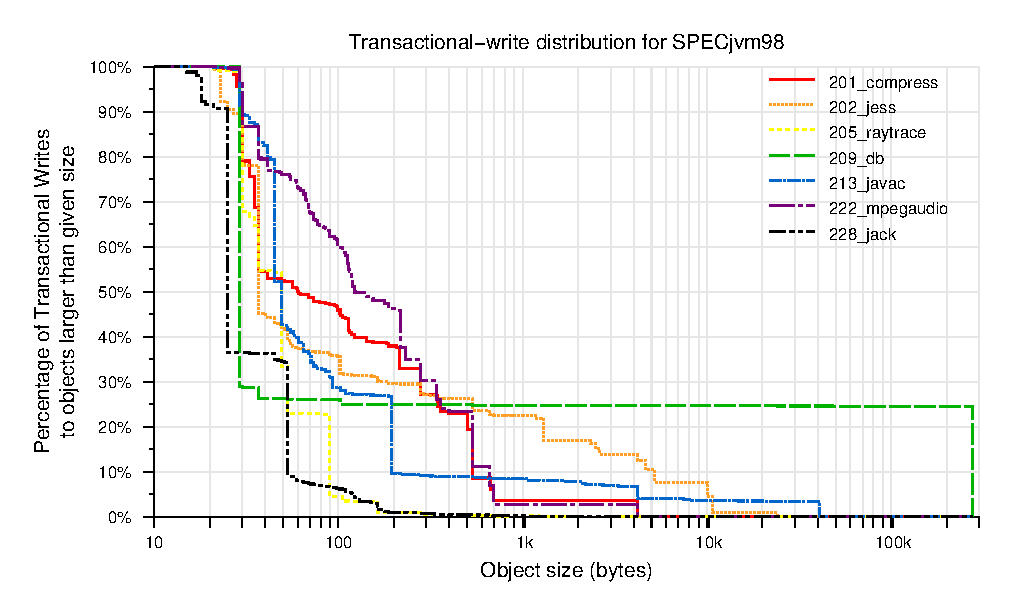
\includegraphics[height=2.75in,clip=true]{Figures/tr-w-all-1}%
\end{center}%
\caption{Proportion of transactional writes to objects equal to or
  smaller than a given size.}
\label{fig:tr-w}%
\end{figure}%
The software transaction system implemented in the previous chapter
clones objects on
transactional writes, so that the previous state of the object can be
restored if the transaction aborts.  \figref{tr-w} shows the object
size distribution of transactional writes for SPECjvm98, and
indicates that over 10\% of writes may be to large objects.
As we've seen in \secref{full-bench}, the copying cost can become
excessive.

The solution I will propose will
represent objects as \defn{functional
  arrays}.  O'Neill and Burton \cite{ONeillBu97} give a fairly
inclusive overview of such algorithms; I've chosen Tyng-Ruey Chuang's
version \cite{Chuang94} of \emph{shallow binding}, which uses
randomized cuts to the version tree to limit the cost of a read to
$O(n)$ in the worst case.  Single-threaded accesses to the array are
$O(1)$.  Our use of functional arrays is single-threaded in the common
case, when transactions do not abort.  Chuang's scheme is attractive
because it limits the worst-case cost of an abort, with very little
added complexity.

In this chapter I will recast the transaction system design of
\charef{stm} as a
``small object protocol,'' then show how to extend it to a ``large
object protocol,'' in the process addressing the large object performance
problems.  The large object protocol will use a lock-free variant of
Chuang's algorithm, which I will present in \secref{lf-fun-arr}.

\section{Basic operations on functional arrays}
Let us begin by reviewing the basic operations on functional arrays.
Functional arrays are \emph{persistent}; that is,
after an element is updated both the new and the old contents of the
array are available for use.  Since arrays are simply maps from
integers (indexes) to values; any functional map datatype (for
example, a functional balanced tree) can be used to implement
functional arrays.

However, the distinguishing characteristic of an imperative array is its
time complexity: $O(1)$ access or update of any element.
Implementing functional arrays with a functional balanced tree yields
$O(\lg n)$ worst-case access or update.\footnote{I will return to
a discussion of operational complexity in \secref{lf-fun-arr}.}

For concreteness, functional arrays have the following three
operations defined:
\begin{itemize}
\item $\funcname{FA-Create}(n)$: Return an array $A$ of size $n$.  The
  contents of the array are initialized to zero.
\item $\funcname{FA-Update}(A, i, v)$: Return an array $A'$ that is
  functionally identical to array $A$ except that
  $\funcname{FA-Read}(A', i)=v$.
  Array $A$ is not destroyed and can be accessed further.
\item $\funcname{FA-Read}(A, i)$: Return $A(i)$ (that is, the
  value of the $i$th element of array $A$).
\end{itemize}
We allow any of these operations to \emph{fail}.  Failed operations
can be safely retried, as all operations are idempotent by definition.

For the moment, consider the following \naive implementation:
\begin{itemize}
\item $\funcname{FA-Create}(n)$: Return an ordinary imperative array of size
  $n$.
\item $\funcname{FA-Update}(A, i, v)$: Create a new imperative array
  $A'$ and copy the contents of $A$ to $A'$.  Set $A'[i]=v$. Return $A'$.
\item $\funcname{FA-Read}(A, i)$: Return $A[i]$.
\end{itemize}
This implementation has $O(1)$ read and $O(n)$ update, so it matches
the performance of imperative arrays only when $n=O(1)$.  I will
therefore call these \emph{small object functional arrays}.  Operations
in this implementation never fail.  Every operation is non-blocking
and no synchronization is necessary, since the imperative arrays are
never mutated after they are created.   In \secref{lf-fun-arr} we will
review better implementations of functional arrays, and present our
own lock-free variant.

\section{A single-object protocol}
\begin{figure}\centering
\includegraphics[width=3.25in,clip=true]{Figures/nb-single-obj}
\caption{Implementing non-blocking single-object concurrent operations
  with functional arrays.}
\label{fig:single-o}
\end{figure}
Given a non-blocking implementation of functional arrays, we can
construct a transaction implementation for single objects.  In
this implementation, fields of at most one object may be referenced
during the execution of the transaction.

I will consider the following two operations on objects:
\begin{itemize}
\item $\funcname{Read}(o, f)$: Read field $f$ of $o$.  We will assume that
  there is a constant mapping function that given a field name
  returns an integer index.  We will write the result of mapping $f$
  as \fref{f}{index}.  For simplicity, and without loss of generality,
  we will assume all fields are of equal size.
\item $\funcname{Write}(o, f, v)$: Write value $v$ to field $f$ of $o$.
\end{itemize}
All other operations on Java objects, such as method dispatch and type
interrogation, can be performed using the immutable {\tt type}
field in the object.  Because the {\tt type} field is never changed
after object creation, non-blocking implementations of operations on
the {\tt type} field are trivial.

As Figure~\ref{fig:single-o} shows, our single-object transaction
implementation represents objects as a pair, combining {\tt type} and a
reference to a functional array.  When not inside a transaction,
object reads and writes are implemented using the
corresponding functional array operation, with the array reference in
the object being updated appropriately:
\begin{itemize}
\item $\funcname{Read}(o, f)$:
  Return $\funcname{FA-Read}(\fref{o}{fields}, \fref{f}{index})$.
\item $\funcname{Write}(o, f, v)$: Replace \fref{o}{fields} with the
  result of \linebreak
  $\funcname{FA-Update}(\fref{o}{fields}, \fref{f}{index}, v)$.
\end{itemize}

The interesting cases are reads and writes inside a transaction.
At entry to our transaction that will access (only) object $o$, we
store \fref{o}{fields} in a local variable $u$.  We create another
local variable $u'$ which we initialize to $u$.  Then our read and
write operations are implemented as:
\begin{itemize}
\item $\funcname{ReadT}(o, f)$:
  Return $\funcname{FA-Read}(u', \fref{f}{index})$.
\item $\funcname{WriteT}(o, f, v)$:
  Update variable $u'$ to the result of \linebreak
  $\funcname{FA-Update}(u', \fref{f}{index}, v)$.
\end{itemize}

At the end of the transaction, we use Compare-And-Swap to atomically
set \fref{o}{fields} to $u'$ if and only if it contained $u$.  If the CAS fails,
we the transaction is aborted (we simply discard $u'$) and we retry.

With our \naive ``small object'' functional arrays, this implementation is
exactly the ``small object protocol'' of Herlihy \cite{Herlihy93}.
Herlihy's protocol is rightly criticized for an excessive amount of
copying.  I will address this with a better implementation of
functional arrays in \secref{lf-fun-arr}.
However, the restriction that only one object
may be referenced within a transaction is overly limiting.  I will
first fix this problem.

\section{Extension to multiple objects}
\begin{figure}\centering
\includegraphics[width=3.25in,clip=true]{Figures/nb-multi-obj}
\caption[Data structures to support non-blocking multi-object
  concurrent operations.]{Data structures to support non-blocking multi-object
  concurrent operations.  Objects point to a linked list of versions,
  which reference transaction identifiers.  Versions created within the
  same execution of a transaction share the same transaction
  identifier.  Version structure also contain pointers to functional
  arrays, which record the values for the fields of the object.
  If no modifications have been made to the object, multiple versions
  in the list may share the same functional array.  (Compare this model
  of a transaction system to our concrete design in \figref{tr-multi-obj-big}.)}
\label{fig:multi-o}
\end{figure}
\begin{figure}
\sis\small%
\renewcommand{\>}{~~}%
\newcommand{\com}[1]{\hfill [{\sl #1}]}%
\begin{tabular}{l}%
$\funcname{Read}(o, f)$:\\
begin\\
retry:\\
\>$u \gets \fref{o}{versions}$ \\
\>$u' \gets \fref{u}{next}$ \\
\>$s  \gets \fref{\fref{u}{owner}}{status}$ \\
\>if ($s=\text{\sl DISCARDED}$) \com{Delete DISCARDED?}\\
\>\>CAS$(u, u', \addr{\fref{o}{versions}})$\\
\>\>goto retry \\
\>else if ($s=\text{\sl COMPLETE}$)\\
\>\>$a \gets \fref{u}{fields}$ \com{$u$ is COMPLETE}\\
\>\>$\fref{u}{next} \gets \text{\bf null}$ \com{Trim version list}\\
\>else\\
\>\>$a \gets \fref{u'}{fields}$ \com{$u'$ is COMPLETE}\\
\>return $\funcname{FA-Read}(a, \fref{f}{index})$ \com{Do the read}\\
end\\
\\
$\funcname{ReadT}(o, f)$:\\
begin\\
\>$u \gets \fref{o}{versions}$\\
\>if ($\var{oid} = \fref{u}{owner}$) \com{My OID should be first}\\
\>\>return $\funcname{FA-Read}(\fref{u}{fields}, \fref{f}{index})$
\com{Do the read}\\
\>else \com{Make me first!}\\
\>\>$u' \gets \fref{u}{next}$\\
\>\>$s  \gets \fref{\fref{u}{owner}}{status}$\\
\>\>if ($s=\text{\sl DISCARDED}$) \com{Delete DISCARDED?}\\
\>\>\>CAS$(u, u', \addr{\fref{o}{versions}})$\\
\>\>else if ($\fref{\var{oid}}{status}=\text{\sl DISCARDED}$)
\com{Am I alive?}\\
\>\>\>fail\\
\>\>else if ($s=\text{\sl IN-PROGRESS}$) \com{Abort IN-PROGRESS?}\\
\>\>\>CAS$(s, \text{\sl DISCARDED}, \addr{\fref{\fref{u}{owner}}{status}})$\\
\>\>else \com{Link new version in:} \\
\>\>\>$\fref{u}{next} \gets \text{\bf null}$ \com{Trim version list}\\
\>\>\>$u' \gets \text{new \tt Version}(\var{oid}, u, \text{\bf null})$
~~~~~~~~~\com{Create new version}\\
\>\>\>if (CAS$(u, u', \addr{\fref{o}{versions}}) \neq \text{\sl FAIL}$)\\
\>\>\>\>$\fref{u'}{fields} \gets \fref{u}{fields}$ \com{Copy old fields}\\
\>\>goto retry\\
end\\
\end{tabular}
\caption{\funcname{Read} and \funcname{ReadT} implementations for the
  multi-object protocol.}\label{fig:reads}
\end{figure}

\begin{figure}
\sis\small%
\renewcommand{\>}{~~}%
\newcommand{\com}[1]{\hfill [{\sl #1}]}%
\begin{tabular}{l}%
$\funcname{Write}(o, f, v)$:\\
begin\\
retry:\\
\>$u  \gets \fref{o}{versions}$\\
\>$u' \gets \fref{u}{next}$\\
\>$s  \gets \fref{\fref{u}{owner}}{status}$\\
\>if ($s=\text{\sl DISCARDED}$) \com{Delete DISCARDED?}\\
\>\>CAS$(u, u', \addr{\fref{o}{versions}})$\\
\>else if ($s=\text{\sl IN-PROGRESS}$) \com{Abort IN-PROGRESS?}\\
\>\>CAS$(s, \text{\sl DISCARDED}, \addr{\fref{\fref{u}{owner}}{status}})$\\
\>else \com{$u$ is COMPLETE}\\
\>\>$\fref{u}{next} \gets \text{\bf null}$ \com{Trim version list}\\
\>\>$a \gets \fref{u}{fields}$\\
\>\>$a' \gets \funcname{FA-Update}(a, \fref{f}{index}, v)$\\
\>\>if (CAS$(a, a', \addr{\fref{u}{fields}}) \neq \text{\sl FAIL}$)
~~~~~~~~~\com{Do the write}\\
\>\>\>return \com{Success!}\\
\>goto retry\\
end\\
\\
$\funcname{WriteT}(o, f, v)$:\\
begin\\
\>$u  \gets \fref{o}{versions}$\\
\>if ($oid = \fref{u}{owner}$) \com{My OID should be first}\\
\>\>$\fref{u}{fields} \gets \funcname{FA-Update}(\fref{u}{fields}, \fref{f}{index}, v)$\com{Do write}\\
\>else \com{Make me first!}\\
\>\>$u' \gets \fref{u}{next}$\\
\>\>$s  \gets \fref{\fref{u}{owner}}{status}$\\
\>\>if ($s=\text{\sl DISCARDED}$) \com{Delete DISCARDED?}\\
\>\>\>CAS$(u, u', \addr{\fref{o}{versions}})$\\
\>\>else if ($\fref{\var{oid}}{status}=\text{\sl DISCARDED}$)
\com{Am I alive?}\\
\>\>\>{\it fail}\\
\>\>else if ($s=\text{\sl IN-PROGRESS}$) \com{Abort IN-PROGRESS?}\\
\>\>\>CAS$(s, \text{\sl DISCARDED}, \addr{\fref{\fref{u}{owner}}{status}})$\\
\>\>else \com{Link new version in:} \\
\>\>\>$\fref{u}{next} \gets \text{\bf null}$ \com{Trim version list}\\
\>\>\>$u' \gets \text{new \tt Version}(\var{oid}, u, \text{\bf null})$
\com{Create new version}\\
\>\>\>if (CAS$(u, u', \addr{\fref{o}{versions}}) \neq \text{\sl FAIL}$)\\
\>\>\>\>$\fref{u'}{fields} \gets \fref{u}{fields}$ \com{Copy old fields}\\
\>\>goto retry\\
end\\
\end{tabular}
\caption{\funcname{Write} and \funcname{WriteT} implementations for the
  multi-object protocol.}\label{fig:writes}
\end{figure}

I extend the implementation to allow the fields of any number of
objects to be accessed during the transaction.
Figure~\ref{fig:multi-o} shows our new object representation.
Compare this to \figref{tr-multi-obj-big}; we've successfully recast our earlier
transaction system design now in terms of operations on an array datatype.
Objects consist of two slots, and the first represents the immutable
{\tt type}, as before.  The second field, {\tt versions}, points to a
linked list of {\tt Version} structures.  The {\tt Version} structures
contain a pointer {\tt fields} to a functional array, and a pointer
{\tt owner} to an \emph{transaction identifier}.  The transaction
identifier contains a single field, {\tt status}, which can be set to
one of three values: \textsl{COMMITTED}, \textsl{IN-PROGRESS}, or
\textsl{ABORTED}.  When the transaction identifier is created, the
status field is initialized to \textsl{IN-PROGRESS}, and it will be
updated exactly once thereafter, to either \textsl{COMMITTED} or
\textsl{ABORTED}.  A \textsl{COMMITTED} transaction identifier never
later becomes \textsl{IN-PROGRESS} or \textsl{ABORTED}, and
a \textsl{ABORTED} transaction identifier never becomes
\textsl{COMMITTED} or \textsl{IN-PROGRESS}.

We create an transaction identifier when we begin or restart a transaction
and place it in a local variable \emph{tid}.  At the end of the
transaction, we use CAS to set \fref{\var{tid}}{status} to
{\sl COMMITTED} if and only if it was {\sl IN-PROGRESS}.  If the CAS is successful,
the transaction has also executed successfully; otherwise
$\fref{\var{tid}}{status}=\text{\sl ABORTED}$ (which indicates that
our transaction has been aborted) and we must back off and retry.
All {\tt Version} structures
created while in the transaction will reference \emph{tid} in
their {\tt owner} field.

Semantically, the current field values for the object will be given by
the first version in 
the versions list whose transaction identifier is {\sl COMMITTED}.
This allows us to link {\sl IN-PROGRESS} versions in at the head of
multiple objects' versions lists and atomically change the values of
all these objects by setting the one common transaction identifier to
{\sl COMMITTED}.  We only allow one {\sl IN-PROGRESS} version on the
versions list, and it must be at the head, so
before we can link a new version at the head we
must ensure that every other version on the list is {\sl ABORTED} or
{\sl COMMITTED}.

Since we will never look past the first {\sl COMMITTED} version in the
versions list, we can free all versions past that point.  In our
presentation of the algorithm, we do this by explicitly setting the
{\tt next} field of every {\sl COMMITTED} version we see to {\bf null};
this allows the versions past that point to be garbage collected.
An optimization would be to have the garbage collector do the list
trimming for us when it does a collection.
% always must read u.next before u.owner.status to ensure we don't
% get caught with a null pointer from a version that just committed.

We don't want to inadvertently chase the null {\tt next} pointer
of a {\sl COMMITTED} version, so we always load the {\tt next}
field of a version \emph{before} we load {\tt owner.status}.  Since
the writes occur in the reverse order ({\sl COMMITTED} to
{\tt owner.status}, then {\bf null} to {\tt next}) we have ensured that
our {\tt next} pointer is valid whenever the status is not {\sl COMMITTED}.

We begin an atomic method with \funcname{TransStart} and attempt to
complete an atomic method with \funcname{TransEnd}.  They are defined as
follows:
\begin{itemize}
\item $\funcname{TransStart}$: create a new transaction identifier, with
  its status initialized to {\sl IN-PROGRESS}.  Assign it to the
  thread-local variable \var{tid}.
\item $\funcname{TransEnd}$:
  If
 $$\text{CAS}(\text{\sl IN-PROGRESS}, \text{\sl COMMITTED},
             \addr{\fref{\var{tid}}{status}})$$
  is successful, the transaction as a whole has completed successfully,
  and can be linearized at the location of the CAS.
  Otherwise, the transaction has been aborted.  Back off and retry from
  \funcname{TransStart}.
\end{itemize}
Pseudo-code describing \funcname{Read}, \funcname{Write}, \funcname{ReadT},
and \funcname{WriteT} is presented in Figures~\ref{fig:reads} and
\ref{fig:writes}.  In the absence of contention, all operations take
constant time plus an invocation of \funcname{FA-Read} or
\funcname{FA-Update}.

\section{Lock-free functional arrays}\label{sec:lf-fun-arr}
\begin{figure}\centering
\includegraphics[width=5in,clip=true]{Figures/chuang}
\caption[Shallow binding scheme for functional arrays.]
  {Shallow binding scheme for functional arrays, from
  \cite[Figure~1]{Chuang94}.}
\label{fig:chuang}
\end{figure}
In this section I will present a lock-free implementation of functional
arrays with $O(1)$ performance in the absence of contention.
The crucial operation is a rotation of a \emph{difference node} with the
main body of the array. Using this implementation of functional arrays
in the multi-object transaction protocol of the previous chapter
will complete our re-implementation of non-blocking transactions,
solving the large object problem.

Let's begin by reviewing the well-known functional array
implementations.  As mentioned previously,
O'Neill and Burton \cite{ONeillBu97} give an
inclusive overview.  Functional array implementations fall generally
into one of three categories: \emph{tree-based}, \emph{fat-elements},
or \emph{shallow-binding}.

Tree-based implementations typically have a logarithmic term in their
complexity.  The simplest is the persistent binary tree with $O(\ln
n)$ look-up time; Chris Okasaki 
\cite{Okasaki95} has implemented a purely-functional random-access list
with $O(\ln i)$ expected lookup time, where $i$ is the index of the
desired element.

Fat-elements implementations have per-element data structures indexed
by a master array. Cohen \cite{Cohen84} hangs a list of
versions from each element in the master array.
O'Neill and Burton \cite{ONeillBu97}, in a more sophisticated
technique, hang a splay tree off each element and achieve $O(1)$
operations for single-threaded use, $O(1)$ amortized cost when
accesses to the array are ``uniform'', and $O(\ln n)$ amortized worst
case time. 

Shallow binding was introduced by Baker \cite{Baker78} as a method to
achieve fast variable lookup in Lisp environments.  Baker clarified
the relationship to functional arrays in \cite{Baker91}.  Shallow
binding is also called \emph{version tree arrays}, \emph{trailer
  arrays}, or \emph{reversible differential lists}.  A typical
drawback of shallow binding is that reads may take $O(u)$ worst-case
time, where $u$ is the number of updates made to the array.  Tyng-Ruey
Chuang \cite{Chuang94} uses randomized cuts to the version tree to limit
the cost of a read to $O(n)$ in the worst case.  Single-threaded
accesses are $O(1)$.

Our use of functional arrays is single-threaded in the common case,
when transactions do not abort.  Chuang's scheme is attractive because
it limits the worst-case cost of an abort, with very little added
complexity.   In this section I will present a lock-free version of
Chuang's randomized algorithm.

In shallow binding, only one version of the functional array (the
\emph{root}) keeps its contents in an imperative array (the
\emph{cache}).   Each of the other versions is represented as a path
of \emph{differential nodes}, where each node describes the
differences between the current array and the previous array.  The
difference is represented as a pair \tuple{\text{\it index},\text{\it value}},
representing the new value to be stored at the specified index.
All paths lead to the root.  An update to the functional array is
simply implemented by adding a differential node pointing to the array it is
updating.

The key to constant-time access for single-threaded use is provided by the read
operation.  A read to the root simply reads the appropriate value from
the cache.  However, a read to a differential node triggers a series
of rotations that swap the direction of differential nodes and result
in the current array acquiring the cache and becoming the new root.
This sequence of rotations is called \emph{re-rooting}, and is
illustrated in Figure~\ref{fig:chuang}.  Each rotation
exchanges the root nodes for a differential node pointing to it, after
which the differential node becomes the new root and the root becomes
a differential node pointing to the new root. The cost of a read is
proportional to its re-rooting length, but after the first read
accesses to the same version are $O(1)$ until the array is re-rooted again.

Shallow binding performs badly if read operations ping-pong between two
widely separated versions of the array, as we will continually
re-root the array from one version to the other.
Chuang's contribution is to provide for \emph{cuts} to the chain of
differential nodes: once in a while we clone the cache and create a
new root instead of performing a rotation.  This operation takes
$O(n)$ time, so we amortize it over $n$ operations by randomly
choosing to perform a cut with probability $1/n$.

\begin{figure}\centering%
\includegraphics[width=5in,clip=true]{Figures/funarr}
\caption[Atomic steps in $\funcname{FA-Rotate}(B)$.]%
 {Atomic steps in $\funcname{FA-Rotate}(B)$.  Time proceeds top-to-bottom
  on the left hand side, and then top-to-bottom on the right.
  Array $A$ is a root node, and $\funcname{FA-Read}(A, x)=z$.
  Array $B$ has the almost the same contents as $A$, but
  $\funcname{FA-Read}(B, x)=y$.}
\label{fig:funarr}
\end{figure}

\begin{figure}\centering%
\sis%
\renewcommand{\>}{~~}%
\newcommand{\com}[1]{\hfill [{\sl #1}]}%
\begin{tabular}{l}%
$\funcname{FA-Update}(A, i, v)$:\\
begin\\
\>$d \gets \text{new DiffNode}(i, v, A)$\\
\>$A'\gets \text{new Array}(\fref{A}{size}, d)$\\
\>return $A'$\\
end\\
\\
$\funcname{FA-Read}(A, i)$:\\
begin\\
retry:\\
\>$d_C \gets \fref{A}{node}$\\
\>if $d_C$ is a cache, then\\
\>\>$v \gets \fref{A}{node}[i]$\\
\>\>if $(\fref{A}{node} \neq d_C)$\com{consistency check}\\
\>\>\>goto retry\\
\>\>return $v$\\
\>else\\
\>\>\funcname{FA-Rotate}(A)\\
\>\>goto retry\\
end\\
\end{tabular}
\caption{Implementation of lock-free functional array using shallow
  binding and randomized cuts (part 1).}
\label{fig:fun-impl1}
\end{figure}
\begin{figure}\centering%
\sis%
\renewcommand{\>}{~~}%
\newcommand{\com}[1]{\hfill [{\sl #1}]}%
\begin{tabular}{l}%
$\funcname{FA-Rotate}(B)$:\\
begin\\
retry:\\
\>$d_B \gets \fref{B}{node}$\com{step (1): assign names as per Figure~\ref{fig:funarr}.}\\
\>$A \gets \fref{d_B}{array}$\\
\>$x \gets \fref{d_B}{index}$\\
\>$y \gets \fref{d_B}{value}$\\
\>$z \gets \funcname{FA-Read}(A, x)$\com{rotates A as side effect}\\
\\
\>$d_C \gets \fref{A}{node}$\\
\>if $d_C$ is not a cache, then \\
\>\>goto retry\\
\\
\>if $(0 = (\text{random} \bmod \fref{A}{size}))$\com{random cut}\\
\>\>$d_C' \gets \text{copy of }d_C$\\
\>\>$d_C'[x] \gets y$\\
\>\>$s\gets\text{DCAS}(d_C, d_C, \addr{\fref{A}{node}}, d_B, d_C', \addr{\fref{B}{node}})$\\
\>\>if $(s \neq \text{\sl SUCCESS})$ goto retry\\
\>\>else return\\
\\
\>$C \gets \text{new Array}(\fref{A}{size}, d_C)$\\
\>$d_A \gets \text{new DiffNode}(x, z, C)$\\
\\
\>$s \gets \text{CAS}(d_C, d_A, \addr{\fref{A}{node}})$\com{step (2)}\\
\>if $(s\neq \text{\sl SUCCESS})$ goto retry\\
\\
\>$s\gets\text{CAS}(A, C, \addr{\fref{d_B}{array}})$\com{step (3)}\\
\>if $(s\neq \text{\sl SUCCESS})$ goto retry\\
\\
\>$s \gets\text{CAS}(C, B, \addr{\fref{d_A}{array}})$\com{step (4)}\\
\>if $(s\neq \text{\sl SUCCESS})$ goto retry\\
\\
\>$s \gets \text{DCAS}(z, y, \addr{d_C[x]},  d_C, d_C, \addr{\fref{C}{node}})$\com{step (5)}\\
\>if $(s\neq \text{\sl SUCCESS})$ goto retry\\
\\
\>$s \gets \text{DCAS}(d_B, d_C, \addr{\fref{B}{node}}, d_C, {\bf nil}, \addr{\fref{C}{node}})$\com{step (6)}\\
\>if $(s\neq \text{\sl SUCCESS})$ goto retry\\
end\\
\end{tabular}
\caption{Implementation of lock-free functional array using shallow
  binding and randomized cuts (part 2).}
\label{fig:fun-impl2}
\end{figure}

Figure~\ref{fig:funarr} shows the data structures used for the
functional array implementation, and the series of atomic steps used
to implement a rotation.  The {\tt Array} class represents a
functional array; it consists of a {\tt size} for the array and a
pointer to a {\tt Node}.  There are two types of nodes: a {\tt
  CacheNode} stores a value for every index in the array, and a {\tt
  DiffNode} stores a single change to an array.  {\tt Array} objects
that point to {\tt CacheNode}s are roots.

In step 1 of the figure, we have a root array $A$ and an
array $B$ whose differential node $d_B$ points to $A$.  The functional
arrays $A$ and $B$ differ in one element: element $x$ of $A$ is $z$,
while element $x$ of $B$ is $y$.  We are about to rotate $B$ to give
it the cache, while linking a differential node to $A$.

Step 2 shows our first atomic action.  We have created a new {\tt
  DiffNode} $d_A$ and a new {\tt Array} $C$ and linked them between
$A$ and its cache.  The {\tt DiffNode} $d_A$ contains the value for
element $x$ contained in the cache, $z$, so there is no change in
the value of $A$.

We continue swinging pointers until step 5, when can finally set
the element $x$ in the cache to $y$.  We perform this operation with a
DCAS operation that checks that $\fref{C}{node}$ is still pointing to
the cache as we expect.  A concurrent rotation would swing
$\fref{C}{node}$ in its step 1.  In general, therefore, the location
pointing to the cache serves as a reservation on the cache.

Thus in step 6 we need to again use DCAS to simultaneously swing
$\fref{C}{node}$ away 
from the cache as we swing $\fref{B}{node}$ to point to the cache.

Figures~\ref{fig:fun-impl1} and \ref{fig:fun-impl2} present pseudocode
for \funcname{FA-Rotate}, \funcname{FA-Read}, and
\funcname{FA-Update}.  The \funcname{FA-Read} procedure also uses the
cache pointer as a reservation, double-checking the cache pointer
after it finishes its read to ensure that the cache hasn't been stolen
from it.

Let us now consider cuts, where \funcname{FA-Read} clones the cache
instead of performing a rotation.   Cuts also check the cache pointer
to protect against concurrent rotations.  But what if the cut occurs
while a rotation is mutating the cache in step 5?  In this case the
only array adjacent to the root is $B$, so the cut must be occurring
during an invocation of $\funcname{FA-Rotate}(B)$.  But then the
differential node $d_B$ will be applied after the cache is copied,
which will safely overwrite the mutation we were concerned about.

With hardware support for small transactions \cite{HerlihyMo93}
we could cheaply perform the entire rotation atomically, instead of
using this six-step approach.


%% \section{Optimizations}
%% Re-rooting is the most complicated part of the functional array
%% algorithm.  It can be optimized in a number of ways.  For example,

%% %unsync rotate for transaction-local data.
%% The first is to recognize that some array versions can only be seen by
%% a single thread.  In particular, when we are working on an {\sl
%%   IN-PROGRESS} operation, all array versions which it creates are
%% unreachable from other threads until the operation is committed.
%% We can add a field {\tt creator} to the {\tt Array} object that records what
%% operation created that version.  If the {\tt creator} field of both
%% $A$ and $B$ contains our own \var{tid} when we begin a rotate, we know
%% that these versions are both thread local

%% .. uh, no.  This doesn't work.

%% % scales method of tagging fields.

\punt{
\section{Performance of functional array implementation}

XXX: continue previous microbenchmarks, as function of object size.
}

%%%%%%%%%%%%%%%%%%%%%


% LocalWords:  Promela microbenchmark Hennessy PowerPC setjmp longjmp runtime
% LocalWords:  subsumption TransactionAbortException mutex unsynchronized gzip
% LocalWords:  SPECjvm multithreaded transactified Transactification renderer
% LocalWords:  javac analyses StringBuffer stwcx transactionally ReaderList gcc
% LocalWords:  readNT writeNT readT writeT ensureWriter checkWriteField inlined
% LocalWords:  inlines inline PowerPC's Sparc StrongARM Classpath backend JNI
% LocalWords:  bytecode desugaring ensureReader desugar superclass NaN JDK jess
% LocalWords:  parameterized datatype Herlihy ensureReader nontransactional UTM
% LocalWords:  transactification mpegaudio raytrace LTM microarchitecture RISC
% LocalWords:  backoff syscall livelock subword subwords lookup Chuang


\footnote{This section is adapted from~\cite{AnanianAsKuLi04},
co-written with Krste Asanovi\'c, Bradley C. Kuszmaul, Charles
E. Leiserson, and Sean Lie.}
\note{Write intro.}

\section{ISA for transactions}\label{sec:isa}
  We first present the
software interface to UTM, and then describe the implementation
details.

\subsubsection{New instructions}

UTM adds two new instructions to a processor's instruction set
architecture:
\begin{description}
\item[\texttt{XBEGIN pc}:] Begin a new transaction.  The
\texttt{pc} argument to \texttt{XBEGIN} specifies
the address of an \defn{abort handler} (e.g., using a PC-relative offset).
If at any time during the execution of a transaction the hardware determines
that the transaction must fail, it immediately rolls back the
processor and memory state to what it was when \texttt{XBEGIN} was
executed, then jumps to \texttt{pc} to execute the abort handler.
 
\item[\texttt{XEND}:] End the current transaction.  If \texttt{XEND}
completes, then the transaction is committed, and all of its
operations appear to be atomic with respect to any other transaction.
\end{description}

Semantically, we can think of an \texttt{XBEGIN} instruction as a
conditional branch to the abort handler.  The \texttt{XBEGIN} for a
transaction that fails has the behavior of a mispredicted branch.
Initially, the processor executes the \texttt{XBEGIN} as a not-taken
branch, falling through into the body of the transaction.  Eventually
the processor realizes that the transaction cannot commit, at which
point it reverts all processor and memory state back to the point of
misprediction and branches to the abort handler.

UTM supports the nesting of transactions by ``subsuming'' the inner
transaction.  For example, within an ``outer'' transaction, a
subroutine may be called that contains an ``inner'' transaction.
UTM simply treats the inner transaction as part of the atomic
region defined by the outer one.  This strategy is correct, because it
maintains the property that the inner transaction executes atomically.
Subsumed nested transactions are implemented by using a counter to
keep track of nesting depth.  If the nesting depth is positive, then
\texttt{XBEGIN} and \texttt{XEND} simply increment and decrement the
counter, respectively, and perform no other transactional bookkeeping.

\subsubsection{Rolling back processor state}

The branch mispredict mechanism in conventional superscalar processors
can roll back register state only for the small window of recent
instructions that have not graduated from the reorder buffer.  To
circumvent the window-size restriction and allow arbitrary rollback
for unbounded transactions, the processor must be modified to retain
an additional snapshot of the architectural register state.  A UTM
processor saves the state of its architectural registers when it
graduates an \texttt{XBEGIN}\@.  The snapshot is retained either until
the transaction aborts, at which point the snapshot is restored into
the architectural registers, or until the matching \texttt{XEND}
graduates indicating that the transaction has committed.

UTM's modifications to the processor core are illustrated in
\figref{snapshot-utm}.  We assume a machine with a unified physical
register file, and so rather than saving the architectural registers
themselves, UTM saves a snapshot of the register-renaming table
and ensures the corresponding physical registers are not reused until
the transaction commits.
The rename stage maintains an additional ``saved'' bit
for each physical register 
to indicate which registers are part of the working
architectural state, and takes a snapshot as
each branch or \texttt{XBEGIN} is decoded and renamed.
When an \texttt{XBEGIN} instruction
graduates, activating the transaction, the associated ``\texttt{S} bit''
snapshot will have bits set
on exactly those registers holding the graduated architectural state.  Physical
registers are normally freed on graduation of a later instruction that
overwrites the same architectural register.  If the \texttt{S} bit on
the snapshot for the active transaction is
set, the physical register is added to a FIFO called a \defn{Register
Reserved List} instead of the normal \defn{Register Free List}.  This
prevents physical registers containing saved data from being
overwritten during a transaction.  When the
transaction's \texttt{XEND} commits, the active snapshot's \texttt{S}
bits are cleared and the Register
Reserved List is drained into the regular Register Free List.  In the
event that the transaction aborts, the saved register-renaming table
is restored and the reorder buffer is rolled back, as in an exception.
After restoring the architectural register state, the branch is taken
to the abort handler.  Even though the processor can internally
speculatively execute ahead through multiple transactions,
transactions only affect the global memory system as instructions
graduate, and hence UTM requires only a single snapshot of the
architectural register state.

%% CSA: do we need to talk about performance implications of
%% running transactions with a smaller effective register set?
%% Our benchmarks in \secref{perf-results} indicate (obliquely)
%% that this is not an issue.

The current transaction abort handler address, nesting depth, and
register snapshot are part of the transactional state.  They are made
visible to the operating system (as additional processor control
registers) to allow them to be saved and restored on context switches.

\section{The LTM implementation}\label{sec:ltm}

%% Points we are trying to make:
%% \begin{itemize}
%% \item 
%% We want to implement something simpler than UTM to understand how
%% something like UTM will behave. It will tell us something about UTM.
%% \item
%% Understand how programs might behave - microbenchmarks, ping-ponging
%% effect. overheads - they are indeed low for the common case, even
%% lower than locks - the point is not to reduce overhead but to show we
%% have low verhead.
%% \item
%% Understand issues with overflow - performance, data structure
%% \item
%% Understand changes to hardware - processor core, caches
%% \item
%% This design is interesting in its own right - it's easy to implement,
%% good first step, good engineering trade off, reduce technology risk,
%% can be implemented in today's processors with low risk.
%% 
%% \end{itemize}

LTM, which stands for ``large
transactional memory,'' stores speculative transactional data in the
cache and detects conflicts using the cache-coherency protocol in much
the same way as the designs by Herlihy and Moss~\cite{HerlihyMo92} and
Knight~\cite{Knight86,Knight89}.  Also, like previous designs, LTM
detects conflicts using the cache coherency protocol.  Unlike previous
designs, however, LTM allows transactional data to overflow from the
cache into a overflow hash table in main memory.  LTM also provides an
architectural state-save mechanism in hardware.


\subsection{Understanding hardware modifications}

This section describes the LTM implementation.  LTM does not
support the truly unbounded transactions---it limits transactions to
the size of physical memory.  Moreover,
LTM neither allows transactions to be moved between processors nor
does it support context switches during a transaction.  The advantage
of cutting corners in this way is that LTM can be implemented by only
modifying the cache and processor core and without making changes to
the memory subsystem.  The truely unbounded scheme presented later in
this chapter builds on the LTM implementation.

Since UTM handles small transactions in the
cache in a similar fashion, LTM provides a useful intermediate step
toward truly unbounded transactions, while maintaining implementation
simplicity.

We implemented LTM in the UVSIM software simulator. UVSIM is an
execution-driven simulator based on RSIM~\cite{PaiRaAd97}.  UVSIM
simulates MIPS R10K~\cite{MIPSR10K} microprocessors in a shared-memory
multiprocessor configuration similar to the SGI Origin 3000.  The
memory is distributed in the system among the processor nodes. Cache
coherency is maintained using a directory based write-invalidate
protocol. For our tests, each UVSIM processor was configured with a
1MB 4-way set-associative L2 cache using 128-byte cache lines.

LTM has the semantics as those described in \charef{isa}.  The
\texttt{XBEGIN} instruction only accepts the \texttt{pc} field for the
abort handler, since LTM does not use a transaction record.  The
remainder of this section describes the modifications to the cache and
processor core needed to support the LTM semantics.

%% This stuff should now be in the UTM section
%% \subsubsection{Instruction set interface and semantics}
%% 
%% LTM uses MIPS as an example baseline instruction set and adds the
%% following instructions to support transactions:
%% \begin{closeitemize}
%% \item \texttt{xBEGIN} mark start of transaction.
%% \item \texttt{xEND} mark end of transaction.
%% \end{closeitemize}
%% 
%% The \texttt{xBEGIN} instruction starts a transaction and specifies the
%% address of an abort handler using a PC-relative offset.  Semantically,
%% \texttt{xBEGIN} can be viewed as a prescient branch which jumps to the
%% abort handler if the subsequent transaction will be aborted, otherwise
%% execution falls through to the next instruction.  
%% 
%% In LTM, when the \texttt{xBEGIN} is executed, the hardware takes a
%% snapshot of the architectural register state and records the abort
%% handler address.  If the following transaction is aborted at any
%% point, the architectural registers are restored, any pending
%% transactional memory updates are revoked, and execution is restarted
%% at the abort handler address.  The abort handler software is
%% responsible for actions to resolve contention, such as backoff and
%% retry.  The simplest contention resolution policy is to point the
%% \texttt{xBEGIN} instruction at itself, causing an aborted transaction
%% to retry immediately with the restored processor and memory state.
%% 
%% The \texttt{xEND} instruction commits a transaction, atomically
%% updating global memory with all transactional stores executed since
%% the last \texttt{xBEGIN}.  The hardware ensures that all transactions
%% are executed atomically when viewed from global memory, and that
%% transactions are committed in a sequentially consistent order.
%% 
%% Normal loads and stores behave differently inside and outside of a
%% transaction.  Normal memory operations are treated as transactional if
%% they are executed while a transaction is pending.  The local thread
%% can see pending transactional updates, but these are not visible in
%% global memory until committed.  Loads and stores executed outside of
%% transaction ({\em non-transactional memory operations}) have the same
%% semantics as they would in a conventional non-transactional machine.
%% Within a transactional machine this is equivalent to them behaving as
%% miniature transactions that consist of a single atomic memory operation
%% that cannot be aborted.  One advantage of handling normal loads and
%% stores in this fashion is that any subroutine can be called from
%% within a transaction, and that subroutine's operations become part of
%% the transaction.  Thus all old binary libraries and programs will work
%% without any changes, which dramatically reduces the cost of migrating
%% to the LTM system.
%% 
%% As a transaction executes, hardware keeps track of the set of memory
%% locations that have been read or written transactionally.  If a second
%% processor attempts operate on one of these locations in a conflicting
%% manner, an abort is triggered.  In general, either the ongoing
%% transaction or the external reader or writer could be aborted.
%% However, LTM adopts a non-obstructive policy of aborting the ongoing
%% transaction on a conflicting read or write from a second processor.
%% Such a policy relies on appropriate backoff and retry mechanisms to
%% avoid livelock or starvation. However, this was implemented in LTM
%% since it can use the existing cache consistency protocol to detect
%% conflicts without any modifications to the protocol. In addition, this
%% non-obstructive policy also supports normal non-transactional loads
%% and stores very naturally.
%% 
%% LTM supports subsumed transactions, where an \texttt{xBEGIN} can be
%% executed while another transaction is already pending.  This enables
%% modular code development, where a subroutine can use transactions
%% oblivious of whether its callers or callees also use transactions.  In
%% LTM, all nested transactions are merged into the outermost transaction
%% so that each processor can have at most one transaction in progress at
%% any time.  Any abort that occurs while executing within the outermost
%% transaction causes the entire outermost transaction to abort. This, in
%% effect, causes all the inner nested transactions to abort as well. The
%% hardware maintains a counter that keeps track of the nesting level.
%% 

\subsubsection{Cache modifications}

\figput[LTM cache modifications.]{cachemods}%
{LTM cache modifications. The T bit indicates if the line is
transactional. The O bit indicates of the set has
overflowed. Overflowed data is stored in a data structure in uncached
DRAM.}

LTM requires only a few small modifications to the cache.  For small
transactions, the cache is used to store the speculative transactional
state. For large transactions, transactional state is spilled into an
overflow data structure in main memory. An additional bit (T) is added
per cache line to indicate if it is transactional. When a
transactional-memory request hits a cache line, the T bit is set. An
additional bit (O) is added per cache set to indicate if it has
overflowed. When a transactional cache line is evicted from the cache
for capacity reasons, the O bit is set on the set.

In LTM, the main memory always contains the original state of any data
being modified transactionally and all speculative transactional state
is stored in the cache and overflow hash table. A transaction is
committed by simply clearing all the T bits in cache and writing back
to memory all overflowed data. Conflicts are detected using the
cache-coherency protocol. When an incoming cache intervention hits a
transactional cache line, the running transaction is aborted. A
transaction is aborted by simply clearing all the T bits and
invalidating all modified transactional cache lines.

The overflow hash table in uncached main memory is maintained by
hardware, but its location and size are set up by the operating
system.  If a request from the processor or a cache intervention misses
on the resident tags of an overflowed set, the overflow hash table
needs to be searched for the requested line. If the requested cache
line is found, it is swapped with a line in the cache set and handled
like a hit.  If the line is not found, it is handled like a miss.
While handling overflows, all incoming cache interventions are stalled
using a NACK-based network protocol.

The LTM hash-table structure uses the low-order bits of the address as
the index and uses linear probing to resolve conflicts. When the
overflow data structure is full, the hardware signals an exception so
that the operating system can increase the size of the hash table and
retry the transaction.

%% In related work, Herlihy and Moss \cite{HerlihyMo92} sketch a scheme
%% for supporting transactions that do not fit within cache by using a
%% hash table that indicates whether software must trap. In contrast,
%% LTM is a hardware-only scheme for transactions that scale to arbitrary
%% size, which now makes technological sense, because the VLSI density is
%% much greater than it was ten years ago when Herlihy and Moss first
%% studied the problem.  In our hardware scheme, the common case stays
%% on-chip, and the uncommon case spills transactions into user-provided
%% memory.
%% 

\subsubsection{Processor modifications}

\figput[LTM processor modifications.]{snapshot}%
{LTM processor modifications. The S bit vector tracks the active
 physical registers. There is an S bit vector snapshot associated with
 each rename table snapshot. The Register Reserved List holds the
 otherwise free physical registers until the transaction commits. The
 LPR field is the next physical register to free (the last physical
 register referenced by the destination architectural register).}
 

LTM requires only minor modifications to the processor core as shown
in \figref{snapshot}. Most modifications are to support the
architectural register state-save that occurs at \texttt{XBEGIN}. A
Register Reserved List FIFO is added and an active physical-register
bit vector (S) with corresponding snapshots are added. The
modifications are minor since LTM uses much of the existing
branch-prediction hardware to implement the state-save mechanism.

\note{Check this against the final version of the HPCA paper.}
LTM uses the S bit vector to mark the physical registers that need to
be saved and does not free them until the transaction commits. On
\texttt{XBEGIN}, a snapshot of the current rename table and the active
S bit vector is taken and saved away. If a physical register marked in
the saved S vector is supposed to be freed before the transaction
commits, it is added to the Register Reserved List instead of the
Register Free List. When the transaction commits, the Register
Reserved List is allowed to drain lazily into the Register Free
List. Therefore, physical registers containing saved data are not
overwritten until after the transaction is committed.

In the event that the transaction aborts, the saved rename table is
restored and the reorder buffer is rolled back as in an exception.
Since none of the saved registers were overwritten, this restores the
architectural register state.

\subsection{Optimizing the common case}

A main goal of LTM and UTM is to run the common case fast. As shown in
\secref{benchmarks}, the common case is when transactions are small
and fit in the cache. Therefore, by using the cache and cache
coherency mechanism to handle small transactions, LTM is able to
execute with almost no overhead over serial code in the common
case. In this section, we discuss qualitatively how the LTM
implementation is optimized for the common case and how similar
techniques are used in UTM. The discussion is broken into the
following three cases: starting, running, committing a transaction.

Starting a transaction in LTM requires virtually no overhead in the
common case since the hardware only needs to record the abort handler
address. No communication with the cache or other external hardware is
necessary. There is the added overhead of decoding the \texttt{XBEGIN}
however that overhead is generally insignificant compared to the cost
of the transaction. Further, instruction decode overhead is much lower
in LTM than with locks. Even schemes where the lock is not actually
held such as SLE have higher decode overhead since they have more
instructions. LTM's low transaction startup overhead is a very good
indicator of the corresponding overhead in UTM since transaction start
up in UTM is virtually the same.

Running a transaction in LTM requires no more overhead than running
the corresponding non-synchronized code in the common case. In LTM,
the T bit is simply set on each transactional cache access. LTM's low
overhead in this case unfortunately does not translate directly to UTM
since UTM modifies the transaction record on each memory
request. However, in the common case the transaction record entry is
also in the cache. Thus all operations are local and no external
communication is needed. Also, in some cases, the cache can respond to
the memory request once the requested data is found. However, if the
request requires data from the transaction record before it can be
serviced, an additional cache lookup is necessary. However, the lookup
is local and thus can be done relatively quickly. \note{Is this
enough?  Seems like the additional lookup in the cache could increase
cache latency significantly} Therefore, the common case overhead of
running a transaction can be minimal even in UTM.

Committing a transaction in LTM has virtually no overhead in the
common case since it can be done in one clock cycle. LTM transaction
commits only requires a simply flash clear of all the transaction bits
in the cache. Similarly, UTM transaction commits only require a single
change of the cached transaction record to ``committed''. UTM
transaction commit also writes the updated values from the transaction
record back to memory. However, this write back can be done lazily in
the background.  Therefore, since transaction commit requires only a
single change in the cache for both LTM and UTM, the overhead is
minimal in both cases.

\subsection{Understanding overflows}

Overflows occur only in the uncommon case
however our studies show that it is important to have a scalable data
structure even though it is used infrequently.

For evaluation, we compiled three versions of the SPECjvm98 benchmark
suite to run under UVSIM using our modified Java compiler. We compiled
a \defn{Base} version that uses no synchronization, a \defn{Locks}
version that uses spin-locks for synchronization, and a \defn{Trans}
version that uses LTM transactions for synchronization. To measure
overheads, we ran these versions of the SPECjvm98 benchmark suite on
one processor of UVSIM.

As described in \secref{spec}, our transactional version uses method
cloning to flatten transactions; we performed the same cloning on the
other compiled versions so that performance improvements due to the
specialization would not be improperly attributed to
transactionification.  The three different benchmark versions were
built from a common code-base using method inlining in GCC\footnote{We
compiled the files generated by FLEX's ``PreciseC'' backend with
\texttt{-O9} for a \texttt{-mips4} target using the
\texttt{n64} api to generate fully-static binaries executable by
UVSIM.}  to remove or replace all invocations of lock and transaction
entry and exit code with appropriate implementations.  No garbage
collection was performed during benchmark runs.


\label{sec:javac}
Our initial results from \charef{efficient} suggested that since
overflows are infrequent, the efficiency of the data structure would
have a negligible effect on overall performance. Therefore, our first
LTM implementation used an unsorted array that required a linear
search on each miss to an overflowed set. The unsorted array was
effective for most of our test cases, as they had less overhead than
locks.  Using LTM with the unsorted array, however, the transactional
version of \texttt{213\_javac} was 14 times slower than the base
version.  Virtually all of the overhead came from handling overflows,
which is not surprising, since the entire application is enclosed in
one large transaction. The large transaction touches 13K cache lines
with 9K lines overflowed.  So, even though only 0.5\% of the
transactional memory operations miss in the cache, each one incurs a
huge search cost. This unexpected slowdown indicated that a naive
unsorted array is insufficient as an overflow data
structure. Therefore, LTM was redesigned to use a hash table to store
overflows.

Since the entire application was enclosed in a transaction, the
\texttt{213\_javac} application was clearly not written to be a
parallel application. However, it is important that an unbounded
transactional memory system be able to support even such applications
with reasonable performance. Therefore, we redesigned LTM to use hash
table as described in \secref{cachemods}.


\begin{figure}
\footnotesize
\begin{center}
\begin{tabular}{l|r|rr|rr}
Benchmark                 &  Base       & Locks         & Trans                  & Time in   & Time in                    \\
application               &  time       & time          & time                   & trans     & overflow                   \\
                          &  (cycles)   & \multicolumn{2}{c|}{(\% of Base time)} & \multicolumn{2}{c}{(\% of Trans time)} \\ \hline
\texttt{200\_check}       &   8.1M      & 124.0\%       & 101.0\%                & 32.5\%     & 0.0085\%                  \\
% \texttt{201\_compress}    & 608.3M      & 102.5\%       & 106.1\%                &  3.8\%     & 4.0\%                     \\
\texttt{202\_jess}        &  75.0M      & 140.9\%       & 108.0\%                & 59.4\%     & 0.0072\%                  \\
\texttt{209\_db}          &  11.8M      & 142.4\%       & 105.2\%                & 54.0\%     & 0\%                       \\
\texttt{213\_javac}       &  30.7M      & 169.9\%       & 114.2\%                & 84.2\%     & 10\%                      \\
\texttt{222\_mpegaudio}   &  99.0M      & 100.3\%       &  99.6\%                &  0.8\%     & 0\%                       \\
\texttt{228\_jack}        & 261.4M      & 175.3\%       & 104.3\%                & 32.1\%     & 0.0056\%                  \\
\end{tabular}
\end{center}
\caption[SPECjvm98 performance on a 1-processor UVSIM simulation.]{%
SPECjvm98 performance on a 1-processor UVSIM simulation.  The {\em
Time in trans} and {\em Time in overflow} are the times spent actually
running a transaction and handling overflows respectively. The input
size is 1. The overflow hash table is 128MB.}
\label{fig:specperf}
\end{figure}

Using LTM with the hash table, the SPECjvm98 application overheads
were much more reasonable as shown in \figref{specperf}.  The hash
table data structure decreased the overhead from a 14x slowdown to
under 15\% in \texttt{213\_javac}. Using the hash table, LTM
transactional overhead is less than locking overhead in all cases.

\punt{
These results indicate that UTM will also have minimal overhead, since
the UTM data structure behaves much like the LTM hash table. When we
miss in the cache, LTM requires one additional access of memory to
index the hash table when there is no conflict. Similarly, UTM
requires one additional access of memory to retrieve the requested
cache line.  UTM may require an additional access of memory, however,
to retrieve the transactional record entry. UTM requires at most one
more access to memory than LTM when there is overflow.  Therefore, the
overflow overhead of UTM will be very similar to that of UTM.
}

\subsection{Understanding program behavior}

\begin{figure}
\begin{center}
\begin{tabular}{c}
\includegraphics{Figures/uvsimCounterRuntime.eps}
%% \includegraphics{uvsimLinkedListRuntime.eps}
\end{tabular}
\end{center}
\caption{\texttt{Counter} performance on UVSIM.}
\label{fig:microbenchperf}
\end{figure}

Using LTM we are able to gain insight into how transactional programs
behave in a transactional memory system such as UTM. Using the
\texttt{Counter} microbenchmark, we found that small transactions are
likely to complete even when contention is high. LTM uses the
cache and cache-coherency protocol to store transactional state and
detect conflicts in the common case. Transactional-memory systems that
use the same technique, such as UTM, all exhibit similar
properties for the common case.

We implemented the \texttt{Counter} parallel application to examine
program behavior for small transactions with high contention. Our
results show that the extremely low overhead of small transactions
enable them to almost always complete even when contention is high.

The \texttt{Counter} microbenchmark has one shared variable that each
processor atomically increments repeatedly with no backoff
policy. Each transaction is only a few instructions long and every
processor attempts to write to the same location repeatedly.  Both a
locking and a transactional version of \texttt{Counter} were run on
UVSIM with LTM, and the results are shown in
\figref{microbenchperf}. In the locking version, there is a global
spin-lock that each processor obtains using a
load-linked/store-conditional (LLSC) sequence from the SGI
synchronization libraries.

The locking version scales poorly, because the LLSC causes many cache
interventions even when the lock cannot be obtained. On the other
hand, the transactional version scales much better, despite having no
backoff policy.  When a transaction obtains a cache line, it is likely
to be able to execute a few more instructions before receiving an
intervention since the network latency is high.  Therefore, small
transactions can start and complete (and perhaps even start and
complete the next transaction) before the cache line is taken away.
Similar behavior is expected from UTM since small transactions
effectively use the cache the same way.

%% \subsubsection{The \texttt{LinkedList} microbenchmark}
%% 
%% We implemented the \texttt{LinkedList} parallel application to examine
%% program behavior for moderately sized transactions with varying
%% contention. Our results show that when contention is low, transactions
%% are very efficient as expected. However, as contention increases, the
%% efficiency is highly dependent on the backoff policy. In some cases,
%% simple backoff policies may be insufficient.
%% 
%% The \texttt{LinkedList} application has an equal number of consumer
%% and producer processors. There is one doubly-linked list for each
%% consumer. Each consumers repeatedly takes items from the head of its
%% list while each producer repeatedly adds items to the tail of a random
%% list. The locking version locks the entire list when adding or
%% removing items. Locks are implemented as in \texttt{Counter}.
%% 
%% For very few processors, transactions perform much better than
%% conventional locks because transactions allow concurrent accesses to
%% the head and the tail of the linked list. However, as the number of
%% processors is increased, the chance that multiple producers will
%% conflict increases.  When \texttt{LinkedList} was first implemented,
%% no backoff policy was used and, as a result, livelock prevented
%% program completion for more than two processors. Then,
%% \texttt{LinkedList} was implemented with binary exponential backoff
%% and \figref{microbenchperf} shows those results. Backoff solved the
%% livelock problem however as the contention increases, the performance
%% of the transactions decreases dramatically. At high contention,
%% transactions are being aborted repeatedly and a lot of time is spent
%% in backoff. In fact, for \texttt{LinkedList} after 32 processors the
%% transactional version is slower than the locking version. This
%% suggests that such a simple backoff policy may be insufficient in high
%% contention.
%% 
%% The \texttt{LinkedList} application illustrates the importance of a
%% good back policy in non-obstructive transactional memory systems such
%% as LTM and UTM.  Such systems do not face the problem of
%% deadlock. However, they must prevent livelock using backoff or other
%% policies. Perhaps there needs to be a forward progress guarantee to
%% get reasonable performance in high contention. This is one of the main
%% challenges that transactional memory schemes such as UTM face.
%% 


%%%%%%%%%%%%%%%%%%%%%%%%%%%%%%%%%%%%%%%%%%%%%%%%%%%%%%%%%%%%%%%%%%
%%%%%%%%%%%%%%%%%%%%%%%%%%%%%%%%%%%%%%%%%%%%%%%%%%%%%%%%%%%%%%%%%%
%-----------------------------------------------------------------
%%%%%%%%%%%%%%%%%%%%%%%%%%%%%%%%%%%%%%%%%%%%%%%%%%%%%%%%%%%%%%%%%%
%%%%%%%%%%%%%%%%%%%%%%%%%%%%%%%%%%%%%%%%%%%%%%%%%%%%%%%%%%%%%%%%%%


\section{The UTM architecture}\label{sec:utm}

This section describes a system called UTM that implements
unbounded transactional memory in hardware.  UTM allows
transactions to grow (nearly) as large as virtual memory.  It also
supports a semantics for nested transactions, where interior
transactions are subsumed into the atomic region represented by the
outer transaction.  Unlike previous schemes that tie a thread's
transactional state to a particular processor and/or cache, UTM
maintains bookkeeping information for a transaction in a
memory-resident data structure, the \defn{transaction log}.  This
enables transactions to survive timeslice interrupts and process
migration from one processor to another.


\subsubsection{Memory state}

Previous HTM systems \cite{Knight86,HerlihyMo93} represent a
transaction partly in the processor and partly in the cache, taking
advantage of the coincidence between the cache-consistency protocol
and the underlying consistency requirements of transactional memory.
Unlike those systems, UTM transactions are represented by a single
\defn{xstate} data structure held in the memory of the system.  The
cache in UTM is used to gain performance, but the correctness of
UTM does not depend on having a cache.  In the following
paragraphs, we first describe the xstate and how the system uses it
assuming there is no caching.  Then, we describe how caching
accelerates xstate operations.

% We uniformly use 'block' to refer to the transaction chunk size.
% block size may or may not be the same as cache-line size.

The xstate is illustrated in \figref{datastruct-entry}.  The xstate
contains a transaction log for each active transaction in the system.
A transaction log is allocated by the operating system for each
thread, and two processor control registers hold the base and bounds
of the currently active thread's log.  Each log consists of a
\defn{commit record} and a vector of \defn{log entries}.  The commit
record maintains the transaction's status: \texttt{PENDING},
\texttt{COMMITTED}, or \texttt{ABORTED}.  Each log entry corresponds
to a block of memory that has been read or written by the transaction.
The entry provides a pointer to the block and the old (backup) value
for the block so that memory can be restored in case the transaction
aborts.  Each log entry also contains a pointer to the commit record
and pointers that form a linked list of all entries in all transaction
logs that refer to the same block.

The final part of the xstate consists of a \defn{log pointer} and one
\defn{RW bit} for each block in memory (and on disk, when paging).  If
the RW bit is \texttt{R}, any transactions that have accessed the
block did so with a load; otherwise, if it is \texttt{W}, the block
may have been the target of a transaction's store.  When a processor
running a transaction reads or writes a block, the block's log pointer
is made to point to a transaction log entry for that block.  Further,
if the access is a write, the RW bit for the block is set to
\texttt{W}.  Whenever another processor references a block that is
already part of a pending transaction, the system consults the RW bit
and log pointer to determine the correct action, for example, to use
the old value, to use the new value, or to abort the transaction.

%% Place these two sentences someplace better?
%% Be sure to keep ``user-level'' as a modifier on programmer, because
%% the OS programmer *can* see the bits.
\punt{The log pointer (a global virtual address) and RW bit are
not visible to the user-level programmer, and in this regard they are
like error-correction bits or cache directory.  On the other hand the
bits are visible to the operating system so that, for example, they
can be paged to disk.  The xstate includes all the active transaction
logs and all the RW bits and log pointers for the entire memory of the
system.}
%% CSA: I cut this and put the details elsewhere.

% CSA: i removed a sentence about needing to consult the transaction
% record if the bit is 'W' because it is unclear: you need to consult
% the transaction record even if the bit is 'R'; for example if you're
% in a different transaction (to make sure you're on the readers list),
% or not in a transaction but you're planning on writing to the block
% (kill all readers)).

% CSA: we either need to specify how the RW bits in full detail, or
% not.  We're getting into trouble because we'll make statements
% about RW bits which don't actually treat some of the cases.  We must
% always think about non-transactional and transactional accesses, and
% four separate modes: untouched by transaction, read by a single
% transaction (upgradable), written by a single transaction, and
% read by multiple transactions.

% CSA: i propose a single bit rather than RW, w/ the following
% meanings:
%   bit   log pointer
%    0       0         -- not involved in xaction.
%    0     somewhere   -- read by a single transaction.
%    1       0         -- read by multiple transactions
%    1     somewhere   -- written by a (single) transaction.

% CSA: we can flip the 'somewhere' cases to make the bit RW again:
% now the key is to allow/recognize the 'read but log pointer 0' case.
%    0       0         -- not involved in xaction.
%    1     somewhere   -- read by a single transaction.
%    1       0         -- read by multiple transactions
%    0     somewhere   -- written by a (single) transaction.

%% XXX: how do i identify the 'mutliple transactions' if the log
%% pointer is null??

% this is likely out-of-scope of this paper.
% the RW bit does not distinguish the 'read by single xaction' and
% 'read by multiple xactions' cases, which is important because we
% probably don't want to have to traverse the readers list if we're
% just writing to a block we read (i.e, increment).

\begin{figure}[b]
\hspace{-0.15cm}
\input{Figures/snapshot.pstex_t}
\caption[UTM processor modifications.]%
{UTM processor modifications. The S bit vector
tracks the active physical registers.  For each rename table snapshot,
there is an associated S bit vector snapshot.  The Register Reserved
List holds the otherwise free physical registers until the transaction
commits.  The LPR field is the next physical register to free (the
last physical register referenced by the destination architectural
register).}
\label{fig:snapshot-utm}
\end{figure}
\begin{figure}[b]
%\centering
\hspace{-1.3cm} % Make the datastruct-entry slide over to the left (it is in the right column, going off the edge)
\input{Figures/datastruct-entry.pstex_t}
\caption[The xstate data structure.]{The xstate data structure.
The transaction log for a transaction contains a commit record and a
vector of log entries.  The log pointer of a block in memory
points to a log entry, which contains the old value of the block and a
pointer to the transaction's commit record.  Two transaction logs
are shown here; generally, the xstate includes the active
transaction logs for the entire system.}
\label{fig:datastruct-entry}
\end{figure}

%\figput{datastruct-entry}{The xstate data structure.  The transaction
%log for a transaction contains a commit record and a vector of log
%entries.  The log pointer of a block in memory points to a log
%entry, which contains the old value of the block and a pointer to the
%transaction's commit record.  Only one transaction log is shown here,
%but generally the xstate includes the active transaction logs in the
%entire system.}

When a processor makes an update as part of a transaction, the new
value is stored in memory and the old value is stored in an entry in
the transaction log.  In principle, there is one log entry for every
load or store performed by the transaction.  If the memory allocated
to the log  is not large enough, the
transaction aborts and the operating system allocates a larger
transaction log and retries the transaction.  When
operating on the same block more than once in a transaction, the
system can avoid writing multiple entries into the transaction log by
checking the log pointer to see whether a log entry for the block
already exists as part of the running transaction.

By following the log pointer to the log entry, then following the log
entry pointer to the commit record, one can determine the transaction
status (pending, committed, or aborted) of each block.  To commit a
transaction, the system simply changes the commit record from
\texttt{PENDING} to \texttt{COMMITTED}.  At this point, a reference to
the block produces the new value stored in memory, albeit after some
delay in chasing pointers to discover that the transaction has been
committed.  To avoid this delay, as well as to free the transaction
log for reuse, the system must clean up after committing.  It does so
by iterating through the log entries, clearing the log pointer for
each block mentioned, thereby finalizing the contents of the block.
Future references to that block will continue to produce the new value
stored in memory, but without the delay of chasing pointers.  To abort
a transaction, the system changes the commit record from
\texttt{PENDING} to \texttt{ABORTED}.  To clean up, it iterates
through the entries, storing the old value back to memory and then
clearing the log pointer.  We chose to store the old value of a block
in the transaction log and the new value in memory, rather than the
reverse, to optimize the case when a transaction commits.  No data
copying is needed to clean up after a commit, only after an abort.

When two or more pending transactions have accessed a block and at
least one of the accesses is a store, the transactions conflict.
Conflicts are detected during operations on memory.  When a
transaction performs a load, the system checks that either the log
pointer refers to an entry in the current transaction log, or else
that the RW bit is \texttt{R} (additionally creating an entry in the
current log for the block if needed).  When a transaction performs a
store, the system checks that no other transaction is referenced by
the log pointer (i.e., that the log pointer is cleared or that the
linked list of log entries corresponding to this block are all
contained in the current transaction log).  If the conflict check
fails, then some of the conflicting transactions are aborted.  To
guarantee forward progress, UTM writes a timestamp into the
transaction log the first time a transaction is attempted.  Then, when
choosing which transactions to abort, older transactions take
priority.  As an alternative, a backoff scheme \cite{MetcalfeBo76}
could also be used.

When a writing transaction wins a conflict, there may be multiple
reading transactions that must be aborted.  These transactions are
found efficiently by following the block's log pointer to an entry and
traversing the linked list found there, which enumerates all entries
for that block in all transaction logs.

\punt{
\note{KA: I wanted to say this but don't actually believe it's true:
A transactional load or store operation may result in the processor
performing many memory accesses to the xstate structure, but the data
structure is designed to allow these to be arbitrarily interleaved
with memory accesses from other ongoing transactions.}
% CSA: i don't think it's true either; at least not obviously.
}

\subsubsection{Caching}

Although UTM can support transactions of unbounded size using the
xstate data structure, multiple memory accesses for each operation may
be required.  Caching is needed to achieve acceptable performance.  In
the common case of a transaction that fits in cache, UTM, like the
earlier proposed HTM systems \cite{Knight86,HerlihyMo93}, monitors the
cache-coherence traffic for the transaction's cache lines to determine
if another processor is performing a conflicting operation.  For
example, when a transaction writes to a memory location, the cache
protocol obtains exclusive ownership on the whole cache block.  New
values can be stored in cache with old values left in memory.  As long
as nothing revokes the ownership of any block, the transaction can
succeed.  Since the contents of the transaction log are undefined
after the transaction commits or aborts, in many cases the system does
not even need to write back a transaction log.  Thus, for a small
transaction that commits without intervention from another
transaction, no additional interprocessor communication is required
beyond the coherence traffic for the nontransactional case.  When the
transaction is too big to fit in cache or interactions with other
transactions are indicated by the cache protocol, the xstate for the
transaction overflows into the ordinary memory hierarchy.  Thus, the
UTM system does not actually need to create a log entry or update
the log pointer for a cached block unless it is evicted.  After a
transaction commits or aborts, the log entries of unspilled cached
blocks can be discarded and the log pointer of each such block can be
marked clean to avoid writeback traffic for the log pointer, which is
no longer needed.  Most of the overhead is borne in the uncommon case,
allowing the common case to run fast.

The in-cache representation of transactional state and the xstate data
structure stored in memory need not match.  The system can optimize
the on-processor representation as long as, at the cache interface, the
view of the xstate is properly maintained.  For convenience, the
transaction block size can match the cache line size.

\subsubsection{System issues}

The goal of UTM is to support transactions that can run for an
indefinite length of time (surviving time slice interrupts), can
migrate from one processor to another along with the rest of a
process's state, and can have footprints bigger than the physical
memory.  Several system issues must be solved for UTM to achieve that
goal.  The main technique that we propose is to treat the xstate as
a system-wide data structure that uses global virtual addresses.

Treating the xstate as data structure directly solves part of the
problem.  For a transaction to run for an indefinite length of time,
it must be able to survive a time-slice interrupt.  By adding the
log pointer to the processor state and storing everything else in a
data structure, it is easy to suspend a transaction and run another
thread with its own transaction.  Similarly, transactions can be
migrated from one processor to another.  The log pointer is
simply part of the thread or process state provided by the operating
system.

UTM can support transactions that are even larger than physical
memory.  The only limitation is how much virtual memory is available
to store both old and new values.  
% \note{We don't strictly need global virtual addresses, the scheme
% outlined below will work for vanilla per-process virtual addresses.
% CSA: added a `might' to this paragraph to reflect this.}
To page the xstate out of main
memory, the UTM data structures might employ global virtual addresses for
their pointers.  Global virtual addresses are system-wide unique
addresses that remain valid even if the referenced pages are paged out
to disk and reloaded in another location.  Typically, systems that
provide global virtual addresses provide an additional level of
address translation, compared to ordinary virtual memory systems.
Hardware first translates a process's virtual address into a global
virtual address.  The global virtual address is then translated into a
physical address.  Multics \cite{BensoussanClDa72} provided user-level
global virtual addressing using segment-offset pairs as the addresses.
The HP Precision Architecture \cite{Lee89} supports global virtual
addresses in a 64-bit RISC processor.

The log pointer and state bits for each user memory block,
while typically not visible to a user-level programmer, are
themselves stored in addressable physical memory to allow the
operating system to page this information to disk.  The location of
the memory holding the log pointer information for a given user data
page is kept in the page table and cached in the TLB.

During execution of a single load or store instruction, the processor can
potentially touch a large number of disparate memory locations in the
xstate, any of which may be paged out to disk.  To ensure forward
progress, either the system must allow load or store instructions to
be restarted in the middle of the xstate traversal, or, if only
precise interrupts are allowed, the operating system must ensure that
all pages required by an xstate traversal can be resident
simultaneously to allow the load or store to complete without page
faults.

UTM assumes that each transaction is a serial instruction stream
beginning with an \texttt{XBEGIN} instruction, ending with a
\texttt{XEND} instruction, and containing only register, memory, and
branch instructions in between.  A fault occurs if an I/O instruction
is executed during a transaction.\punt{\footnote{Implementing atomic file or
database operations requires higher-level programming, which might use
the transactional memory as an implementation tool, but which is not
directly supported by the hardware.}}

%% \note{Didn't talk about initializing the transaction log: How does
%% the time stamp get filled in?  How is the size of the transaction
%% record specified?  --Bradley}

%% CSA: I think that, when we get around to figuring out how to
%% save/restore the reserved registers on a context-switch, we'll
%% discover that a software-only mechanism makes more sense.
%%
%% KA: Don't agree - it's easy for software to see the snapshot.  Just
%% provide an alternate register space that's read/written using the
%% snapshot rename map.
%%
%% CSA: is recreating a saved register set as easy? (i.e context
%% switch from non-transactional to transactional context)
%%
%% KA: Yup, just write the transactional register snapshot from the OS before
%% jumping back to the user thread.
%%
%% CSA: Which presumably allocates new 's bit set' shadow registers
%% for each architectural register as needed.

% The processor contains hardware support for saving the register state
% into \defn{shadow registers}, which are used to roll back the
% processor state when a transaction fails.  Transaction failures also
% cause a jump to a programmer-defined \defn{abort handler}, which
% may retry the transaction.  The processor maintains bookkeeping
% information for a transaction in a software-specified
% \defn{transaction log} in memory.  One part of the transaction log, called the
% \defn{commit record}, indicates to the hardware whether the
% transaction is pending, committed, or aborted.  After the transaction
% commits or aborts, the contents of the transaction log are undefined.

%% CSA: KA rewrote around the above paragraph.  I readded \defns to
%% the various places where the terms in the above are first
%% mentioned; may want to look at the ``abort handler'' defn, because
%% we only implicitly define the term at that point.

\section{Evaluation}

\section{Making UTM fast}

\section{Calling-convention and function issues}


\section{A hybrid transaction implementation}\label{sec:hybrid}

\begin{figure}[t]\begin{center}%
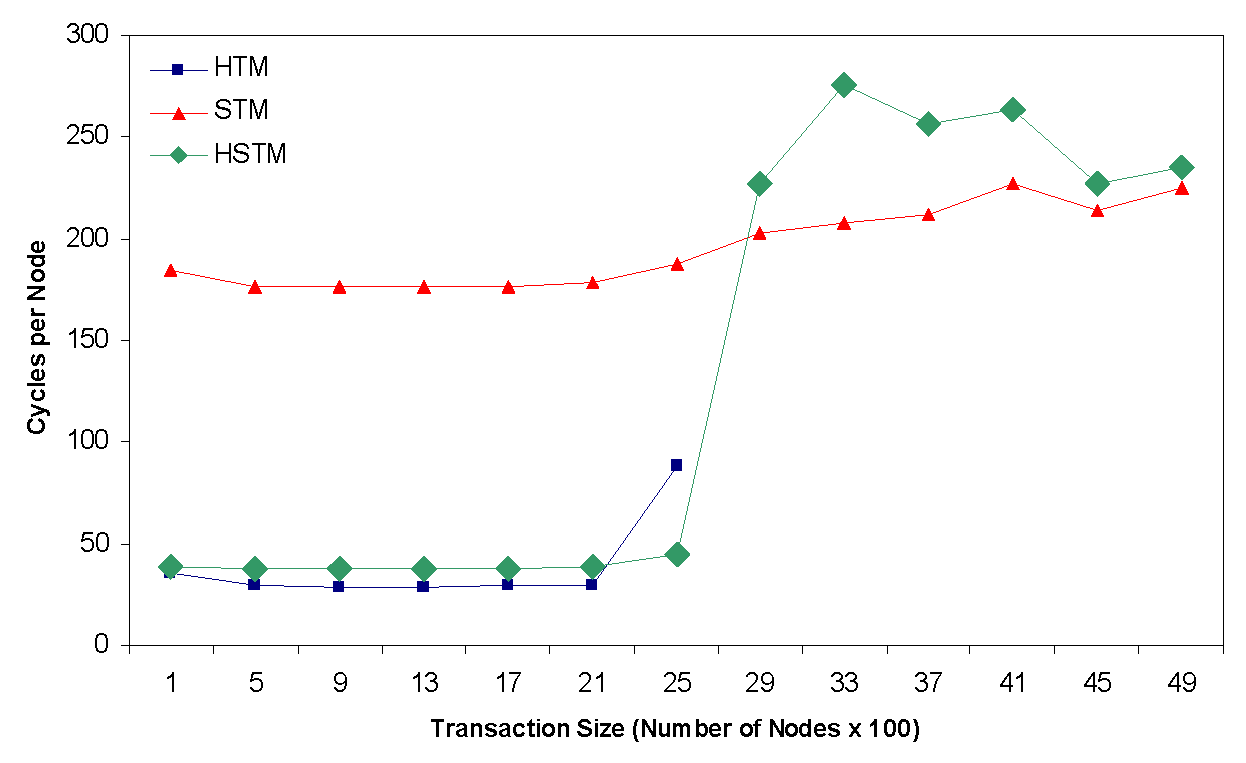
\includegraphics[width=3.25in,clip=true]{Figures/sean_lie_6b}%
\end{center}%
\caption[Hybrid performance on simple queue benchmark.]
{Performance (in cycles per node push on a simple queue
  benchmark) of LTM~\cite{AnanianAsKuLeLi04} (HTM), the
  object-based system presented in this paper (STM) and a hybrid
  scheme (HSTM).}%
\label{fig:hybrid}%
\end{figure}
It is worth considering if a low-level HTM can yield benefits other
than efficient implementations of large-object operations.  In fact,
\figref{hybrid} presents research showing that we can combine the
strengths of our object-based software transaction system with a
fast bounded-size HTM.  In the figure, combining the systems is done
in the most simple-minded way: all transactions are begun in
LTM~\cite{AnanianAsKuLeLi04},
and after any abort the transaction is restarted in the
object-based software system.
  The field flag mechanism described in
\secref{flagfield} ensures that software transactions properly abort
conflicting hardware transactions --- when the software scribbles
\FLAG over the original field the hardware will detect the conflict.
Hardware transactions must perform
the \texttt{ReadNT} and \texttt{WriteNT} algorithms to ensure they
interact properly with concurrent software transactions, although these
checks can be done in software (they do not need to be part of the
hardware HTM mechanism).  In the figure, the read barriers were done
in software, and caused a 2.2x slowdown for the (very small) hardware
transactions.  This is a pessimistic figure: no special effort was
made to tune code or otherwise minimize slowdown, and the processor
simulated had limited ability to exploit ILP (2 ALUs and 4-instruction
issue width).  Even so, the read barriers might be a worthwhile target
for hardware support \cite{ClickTeWo05}.

As a fortuitous synergy, hardware support for small transactions may
also be used to implement the software transaction implementation's
Load Linked/Store Conditional sequences, which may not
otherwise be available on a target processor.


\punt{
\chapter{Extending the hardware}\label{cha:htmplus}
\epigraphhead[70]{\epigraph{%
To create a new standard, it takes something that's not just a little
bit different; it takes something that's really new and really
captures people's imagination\ldots.}{\textit{Bill Gates}, 1984.}}
%%%%%%%%%% Extending the hardware section %%%%%%%%%%555

% First: do we want to?  Next section should how to make software hybrid.

\section{Adding partial rollback}
\subsection{LTM}
% keep a log(n) bit 'nesting level' with each transaction
% bulk decremember nesting level on commit.
% is this really needed?  Why not just 'checkpoints'?
% numbering system: what we really want to do is breadth-first
% numbering of the tree, so that we have well-spaced checkpoints.

\subsection{UTM}
% think about implications here.

\section{Making abort handlers more general}
% calling-convention and function issues.
% save registers in software
% do aborts in software
% this lets us add custom compensation code.
% what environment?  just pick one.


}

\punt{
\epigraphhead[70]{\epigraph{%
Hybrids are often named by the portmanteau method, combining the names
of the two parent species. For example, a zeedonk is a cross between a
zebra and a donkey.}{\textit{Wikipedia}, ``Hybrid''}}

% dual-path coding: publishable paper: try in hw, fall back to software


\chapter{Compiler optimizations and type systems}
% Optimizations and type systems.
\section{Closing the semantic gap}\label{sec:safe-transactify}

}

% 'Challenges' chapter.
In this section we will review objections that have been raised to
straightforward or na{\"\i}ve transaction implementations.
Some of these objections do not apply to our implementation;
discussion of these may further illuminate our design choices.
Others apply to certain situations, and should be kept in mind when
creating applications.  Some of the problems raised remain unsolved,
and are the subject of future work; for these we will attempt to sketch
research directions.

\section{Performance isolation}
Zilles and Flint~\cite{ZillesFl05} identified
\defn{\indexed{performance isolation}} as a potential issue for
transaction implementations.  In a system with performance isolation,
the execution of one task (process, thread, transaction) should
complete in an amount of time which is independent of the execution of
other tasks (processes, threads, transactions) in the system.  For
a system with N processors, it is ideal if a task is guaranteed to
complete at least as quickly as it would running alone on 1
processor.

It is obvious that most common systems do not provide any guarantee of
performance isolation: on a typical multi-user system, the execution
of a given task can be made arbitrarily slow by the concurrent
execution of competing tasks.\footnote{Grunwald and Ghiasi call this a
``microarchitectural denial of service'' attack~\cite{GrunwaldGh02}.}
However, a nontransactional system can
be constructed with a good deal of performance isolation by
appropriately restricting the processes that can be run and the
resources they consume.

Zilles and Flint object that many transactional systems are
constructed such that a single large transaction may monopolize the
atomicity resources such that no other transactions may commit.  By
opening a transaction, touching a large number of memory locations,
and then never closing the transaction, a malicious application may
deny service to all concurrent applications in a transaction system.

Transaction systems provide a solution not available to systems with
lock-based concurrency, however: the offending transaction can be
safely aborted at any point to allow the other transactions to
progress.

\section{Progress guarantees}\label{sec:progress}\index{progress guarantees}
Progress guarantees are closely related to performance isolation, and
Zilles and Flint examine these in the same paper.

\section{The semantic gap}\label{sec:semantic}
Blundell, Lewis, and Martin~\cite{BlundellLeMa05}\ldots

\section{I/O}
\section{OS interactions}


\chapter{Related work}\label{cha:related}
\epigraphhead[70]{\epigraph{%
Everything in the universe relates to [transactions], one way or another,
given enough ingenuity on the part of the interpreter.
}{\textit{Principia Discordia} (amended)}}

A number of researchers have been investigating transactional memory
systems.  This thesis is the first to present a hybrid hardware/software
model-checked non-blocking
object-oriented system that allows co-existence of non-transactional and
transactional accesses to a dynamic set of object fields.
\note{Martin wants citations here: ask him about this?}

\section{Non-blocking synchronization}\label{sec:nb-sync}

Lamport presented the first alternative to synchronization via mutual
exclusion in \cite{Lamport77}, for a limited situation involving a single
writer and multiple readers.  Lamport's technique relies on reading
guard elements in an order opposite to that in which they are written,
guaranteeing that a consistent data snapshot can be recognized.  The
writer always completes its part of the algorithm in a constant number
of steps; readers are guaranteed to complete only in the absence of
concurrent writes.

Herlihy formalized \emph{wait-free} implementations of
concurrent data objects in \cite{Herlihy88}.  A wait-free implementation
guarantees that any process can complete any operation in a finite
number of steps, regardless of the activities of other processes.
Lamport's algorithm is not wait-free
because readers can be delayed indefinitely.

Massalin and Pu introduced the term \emph{lock-free} to describe 
algorithms with weaker progress guarantees.
A lock-free implementation guarantees only that \emph{some}
process will complete in a finite number of steps
\cite{MassalinPu91}.  Unlike a wait-free implementation,
lock-freedom allows starvation.  Since other simple techniques can be
layered to prevent starvation (for example, exponential backoff),
simple lock-free implementations are usually seen as worthwhile practical
alternatives to more complex wait-free implementations.

An even weaker criterion, \emph{obstruction-freedom}, was introduced
by Herlihy, Luchangco, and Moir in \cite{HerlihyLuMo03}.
Obstruction-freedom only guarantees progress for threads executing in
isolation; that is, although other threads may have partially
completed operations, no other thread may take a step until the
isolated thread completes.  Obstruction-freedom not only allows
starvation of a particular thread, it allows contention among threads
to halt all progress in all threads
indefinitely.  External mechanisms are used to reduce contention
(thus, achieve progress) including backoff, queueing, or timestamping.

We will use the term \emph{non-blocking} to describe
generally any synchronization mechanism that doesn't rely on mutual
exclusion or locking, including wait-free, lock-free,
and obstruction-free implementations.
We will be concerned mainly with lock-free algorithms.%
\footnote{Note that some authors use ``non-blocking'' and
  ``lock-free'' as synonyms, usually meaning what we here call
  \emph{lock-free}.  Others exchange our definitions for ``lock-free''
  and ``non-blocking'', using lock-free as a generic term and non-blocking
  to describe a specific class of implementations.  As there is
  variation in the field, we choose to use the parallel construction
  \emph{wait-free}, \emph{lock-free}, and \emph{obstruction-free} for
  our three specific progress criteria, and the dissimilar
  \emph{non-blocking} for the general class.}

\section{Efficiency}\label{sec:efficiency}
Herlihy presented the first \emph{universal} method for wait-free
concurrent implementation of an arbitrary sequential object
\cite{Herlihy88,Herlihy91}.  This original method was based on
a \emph{fetch-and-cons} primitive, which atomically places
an item on the head of a list and returns the list of items following
it; all concurrent primitives capable of solving the
$n$-process consensus problem---\emph{universal} primitives---were
shown powerful enough to implement \emph{fetch-and-cons}.
In Herlihy's method, 
every sequential operation is translated into two steps.  In the first,
\emph{fetch-and-cons} is used to place the name and arguments of the
operation to be performed
at the head of a list, returning the other operations on the list.
Since the state
of a deterministic object is completely determined by the history of
operations performed on it, applying the operations returned
in order from last to first is sufficient to locally reconstruct the
object state 
prior to our operation.
We then use the prior state to compute the result of our operation
without requiring further synchronization with the other processes.

This first universal method was not very practical, a shortcoming
which Herlihy soon addressed \cite{Herlihy93}.  In addition, his revised universal
method can be made lock-free, rather than wait-free, resulting in
improved performance.  In the lock-free version of this method,
objects contain a shared variable
holding a pointer to their current state.  Processes begin by loading
the current state pointer and then copying the referenced state to a
local copy.  The sequential operation is performed on the
copy, and then if the object's shared state pointer is unchanged from
its initial load it is atomically swung to point at the updated state.

Herlihy called this the ``small object protocol'' because the object
copying overhead is prohibitive unless the object is small enough to
be copied efficiently (in, say, $O(1)$ time).  He also presented a
``large object protocol'' which requires the programmer to
manually break the object into small blocks, after which the small
object protocol can be employed. 
[This trouble with large objects is
common to many non-blocking implementations; our solution is presented
in \charef{largeobj}.]

Barnes provided the first universal non-blocking implementation
method that avoids object copying \cite{Barnes93}.  He eliminates the
need to store ``old'' object
state in case of operation failure by having all threads cooperate to
apply operations.  For example, if the first processor begins an operation
and then halts, another processor will complete the operation of the first
before applying its own.  Barnes proposes to accomplish the
cooperation by creating a parallel state machine for each operation,
so that each thread can independently try to advance the machine from state
to state and thus advance incomplete operations.%
\footnote{It is interesting to note that Barnes' cooperative method
  for non-blocking 
  situation plays out in a real-time system very similarly to priority
  inheritance for locking synchronization.}
Although this avoids
copying state, the lock-step cooperative process is extremely
cumbersome and does not appear to have ever been implemented.
Furthermore, it does not protect against errors in the implementation
of the operations, which could cause \emph{every} thread to fail in turn
as one by one they attempt to execute a buggy operation.

Alemany and Felten \cite{AlemanyFe92} identified two factors hindering the
performance of non-blocking algorithms to date: resources wasted by operations
that fail, and the cost of data copying.  Unfortunately, they
proceeded to
``solve'' these problems by ignoring short delays and failures and
using operating system support to handle delays caused by
context switches, page faults, and
I/O operations.  This works in some situations, but obviously suffers
from a bootstrapping problem as the means to implement an operating system.

Although lock-free implementations are usually assumed to be more
efficient that wait-free implementations, LaMarca \cite{LaMarca94}
showed experimental evidence that Herlihy's simple
wait-free protocol scales very well on parallel machines.
When more than about twenty threads are involved, the wait-free
protocol becomes
faster than Herlihy's lock-free small-object protocol, three OS-aided
protocols of LaMarca and Alemany and Felten, and a
\emph{test-and-Compare\&Swap} spin-lock.

% Afek et al have a somewhat complicated improved wait-free method.

% Transactional memories?
\section{Transactional Memory systems}\label{sec:tm}

Transactions are described in the database context by Gray
\cite{Gray81b}, and \cite{GrayRe93} contains a thorough treatment of
database issues.  Hardware Transactional Memory (HTM) was first
proposed by Knight~\cite{Knight86},
and Herlihy and Moss coined the term ``transactional memory'' and
proposed HTM in the context of lock-free data
structures~\cite{HerlihyMo92,HerlihyMo93}.  The BBN
Pluribus~\cite[Ch.~23]{SiewiorekBeNe82} provided transactions, with an
architectural limit on the size of a transaction.  Experience with
Pluribus showed that the headaches of programming correctly with such
limits can be at least as challenging as using locks.  The
\defn{Oklahoma Update} is another variation on transactional
operations with an architectural limit on the number of values in a
transaction~\cite{StoneStHe93}.

Transactional memory is sometimes described as an extension of
Load-Linked/Store-Conditional \cite{JensenHaBr87} and other atomic
instruction sequences.  In fact, some CISC machines, such as the VAX,
had complex atomic instructions such as enqueue and
dequeue~\cite{Digital96}.

Of particular relevance are \defn{Speculative Lock
Elision} (SLE) \cite{RajwarGo01} and \defn{Transactional Lock Removal}
(TLR) \cite{RajwarGo02}, which speculatively identify locks and use
the cache to give the appearance of atomicity.  SLE and TLR handle
mutual exclusion through a standard programmer interface (locks),
dynamically translating locks into transactional regions.  My
research thrust differs from theirs in that I hope to free
programmers from the protocol complexities of locking, not just
optimize existing practice.  The quantitative results presented in
this thesis confirm their finding that transactional hardware can be
more efficient than locks.

Martinez and Torrellas proposed \defn{Speculative Synchronization}
\cite{MartinezTo02}, which allows some threads to execute atomic
regions of code speculatively, using locks, while guaranteeing forward
progress by maintaining a nonspeculative thread.  These techniques
gain many of the performance advantages of transactional memory, but
they still require new code to obey a locking protocol to avoid
deadlock.

The recent work on \defn{Transactional memory Coherence and
Consistency} (TCC)~\cite{HammondWoCh04} is also relevant to our work.
TCC uses a broadcast bus to implement the transaction protocols,
performing all the writes of a particular transaction in one atomic
bus operation.  This strategy limits scalability, whereas both the UTM and
LTM proposals in \charef{htm}
can employ scalable cache-consistency protocols to implement
transactions.  TCC affirms the conclusion we draw from our own
\figref{tr-sz-all}: most transactions are small, but some are very large.  TCC
supports large transactions by locking the broadcast bus and stalling
all other processors when any processor buffer overflows, whereas UTM
and LTM allow overlapped execution of multiple large transactions with
local overflow buffers.  TCC is similar to LTM in that transactions
are bound to processor state and cannot extend across page faults,
timer interrupts, or thread migrations.

\note{Insert VTM reference here \cite{RajwarHeLa05}.}

Several software transaction systems have been proposed.  Some constrain the
programmer and make transactions difficult to use.  All have
relatively high overheads, which make transactions unattractive for
uniprocessor and small SMP systems. [Once the number of processors is
large enough, the increased parallelism that can be provided by
optimistic transactions may cancel out the performance penalty of
their use.]

The first proposal for software transactional memory was proposed by
Shavit and Touitou \cite{ShavitTo95}; their system requires that all
input and output locations touched by a transaction be known in
advance, which limits its application.  It performs at least 10
fetches and 4 stores per location accessed (not counting the loads and
stores directly required by the computation).  The benchmarks
presented were run on between 10 and 64 processors.

Rudys and Wallach \cite{RudysWa02} proposed a copying-based
transaction system to allow rollback of hostile codelets.
They show an order of magnitude slowdown for field and array
accesses, and 6x to 23x slowdown on their benchmarks.

Herlihy, Luchango, Moss, and Scherer's scheme \cite{HerlihyLuMoSc03}
allows transactions to touch a dynamic set of memory locations;
however the user still has to explicitly \emph{open} every object touched
before it can be used in a transaction.  This implementation is based
on object copying, and so has poor performance for large objects and
arrays.  Not including work necessary to copy objects involved in
writes, they require $O(R(R+W))$ work to open $R$ objects for reading
and $W$ objects for writing, which may be quadratic in the number of objects
involved in the transaction.   A list insertion benchmark that they
present shows 9x slowdown over a locking scheme, although they beat the locking
implementation when more than 5-10 processors are active.  They
present benchmark data with up to 576 threads on 72 processors.

Harris and Fraser built a software transaction system on a flat
word-oriented transactional memory abstraction \cite{HarrisFr03},
roughly similar to simulating Herlihy's original hardware
transactional memory proposal in software.  This avoids problems with
large objects.  Performing $m$ memory operations touching $l$ distinct
locations costs at least $m+l$ extra reads and $l+1$ CAS operations, in
addition to the reads and writes required by the computation.
They appear to execute about twice as slowly as a locking
implementation on some microbenchmarks.  They benchmark on a
4-processor as well as a 106-processor machine; their crossover point
(at which the blocking overhead of locks matches the software
transaction overhead) is around 4 processors.
Note that Harris and Fraser do not address the problem of
concurrent non-transactional operations on locations involved in a
transaction.  Java synchronization allows such concurrent operations,
with semantics given by the Java memory model \cite{MansonPu02}.
We support these operations safely using the mechanisms presented in
\charef{stm}.

Programmers will be reluctant to use transactions to synchronize their
code when it results in their code running more slowly on the uniprocessor
and small-SMP systems that are most common today.

Herlihy and Moss \cite{HerlihyMo93} suggested that small transactions
might be handled in cache with overflows handled by software.  These
software overflows must interact with the transactional hardware in
the same way that the hardware interacts with itself, however.
In \secref{hybrid} we presented just such a system.


%%%%%%%%%%%%%%%%%%%%%%%%%%%%%%%%%%%%%%%%%%%%%%%%
\section{Language-level approaches to synchronization}
\begin{figure}
{\samepage\it\sis%
\begin{tabular}{l}%
{\bf const} myDirectory == {\bf object} oneEntryDirectory\\
~~{\bf export} Store, Lookup\\
~~{\bf monitor}\\
~~~~{\bf var} name : String\\
~~~~{\bf var} AnObject : Any\\
\\
~~~~{\bf operation} Store [ n : String, o : Any ]\\
~~~~~~name $\gets$ n\\
~~~~~~AnObject $\gets$ o\\
~~~~{\bf end} Store
\\
~~~~{\bf function} Lookup [ n : String ] $\to$ [ o : Any ]\\
~~~~~~{\bf if} n = name\\
~~~~~~~~{\bf then} o $\gets$ AnObject\\
~~~~~~~~{\bf else} o $\gets$ {\bf nil}\\
~~~~~~{\bf end if}\\
~~~~{\bf end} Lookup\\
\\
~~~~{\bf initially}\\
~~~~~~name $\gets$ {\bf nil}\\
~~~~~~AnObject $\gets$ {\bf nil}\\
~~~~{\bf end initially}\\
\\
~~{\bf end monitor}\\
{\bf end} oneEntryDirectory
\end{tabular}
}
\caption[A directory object in Emerald, illustrating the use of
 monitor synchronization.]
 {A directory object in Emerald, from \cite{BlackHuJuLe86},
  illustrating the use of monitor synchronization.\index{Monitor synchronization}\index{Synchronization!monitor}}
\label{fig:emerald-dir}
\end{figure}

\begin{figure}
{\ttfamily\sis\small%
\begin{tabular}{l}
class Account \{\\
\\
~~int balance = 0;\\
\\
~~{\bf atomic} int deposit(int amt) \{\\
~~~~int t = this.balance;\\
~~~~t = t + amt;\\
~~~~this.balance = t;\\
~~~~return t;\\
~~\}\\
\\
~~{\bf atomic} int readBalance() \{\\
~~~~return this.balance;\\
~~\}\\
\\
~~{\bf atomic} int withdraw(int amt) \{\\
~~~~int t = this.balance;\\
~~~~t = t - amt;\\
~~~~this.balance = t;\\
~~~~return t;\\
~~\}\\
\\
\}\\
\end{tabular}
}\vspace{.2in}
\caption[A simple bank account object
  illustrating the use of the \atomic modifier.]
 {A simple bank account object, adapted from \cite{FlanaganQa03},
  illustrating the use of the \atomic modifier.}
\label{fig:atomic}
\end{figure}

Our work on integrating transactions into the Java programming
language is related to prior work on integrating synchronization
mechanisms for multiprogramming, and in particular, to prior work on
synchronization in an object-oriented framework.

\index{Emerald|(}\label{sec:emerald}
The Emerald system \cite{BlackHuJuLe86,JulSt91} introduced
\defnlti{Monitored objects} for synchronization.  Emerald code to
implement a simple directory object is shown in
Figure~\ref{fig:emerald-dir}.  Each object is associated with
Hoare-style monitor, which provides mutual exclusion and process
signaling.  Each Emerald object is divided into a monitored part and
a non-monitored part.  Variables declared in the monitored part are
shared, and access to them from methods in the non-monitored part is
prohibited---although non-monitored methods may call monitored methods
to effect the access.  Methods in the monitored part acquire the monitor lock
associated with the receiver object before entry and release it on
exit, providing for mutual exclusion and safe update of the shared
variables.  Monitored objects naturally integrate synchronization into
the object model.

Unlike Emerald monitored objects, where methods can only acquire the
monitor of their receiver and where restricted access to shared
variables is enforced by the compiler, Java implements a loose
variant where any monitor may be explicitly acquired and no shared
variable protection exists.  As a default, however, Java methods
declared with the {\tt synchronized} keyword behave like Emerald
monitored methods,
ensuring that the monitor lock of their receiver is held during execution.

Java's synchronization primitives arguably allow for more efficient
concurrent code than Emerald's---for example, Java objects can use
multiple locks to
protect disjoint sets of fields, and coarse-grain locks can be used
which protect multiple objects---but Java is also more prone to programmer
error.  However, even Emerald's restrictive
monitored objects are not sufficient to prevent data races.  As a
simple example, imagine that an object provided two monitored methods
{\tt read} and {\tt write} which accessed a shared variable.
Non-monitored code can call {\tt read}, increment the value returned,
and then call {\tt write}, creating a classic race condition scenario.
The atomicity of the parts is not sufficient to guarantee atomicity of
the whole \cite{FlanaganQa03}.
\note{``Composability'': cite PPoPP paper \cite{HarrisMaPeHe05}?}
\index{Emerald|)}

This suggests that a better model for synchronization in
object-oriented systems is \defnlti{Atomicity}.  Figure~\ref{fig:atomic}
shows Java extended with an \atomic keyword to implement an
object representing a bank account.  Rather than explicitly
synchronizing on locks, I simply require that the methods marked
\atomic execute atomically with respect to other threads in the
system; that is, that every execution of the program computes the same
result as some execution where all atomic methods were run \emph{in
  isolation} at a certain point in time, called the
\defni{Linearization point}, between their invocation and return.
Note that
atomic methods invoked directly or indirectly from an atomic
method are subsumed by it: if the outermost method appears atomic,
then by definition all inner method invocations will also appear atomic.
Flanagan and Qadeer provide a more formal semantics in \cite{FlanaganQa03}.
Atomic methods can be analyzed using sequential reasoning techniques, which
significantly simplifies reasoning about program correctness.

Atomic methods can be implemented using locks.  A simple if inefficient
implementation would simply acquire a single global lock during
the execution of every atomic method.  Flanagan and Qadeer
\cite{FlanaganQa03} present a more sophisticated technique that proves that
a given implementation using standard Java monitors correctly
guarantees method atomicity.

The transaction implementations presented in this thesis will use
non-blocking synchronization to implement atomic methods.


% LocalWords:  atomicity transactional linearization SMP LTM UTM TCC backoff
% LocalWords:  Herlihy


%\chapter{Conclusion}
\chapter{Conclusion}\label{cha:concl}
\epigraphhead[70]{\epigraph{%
``Begin at the beginning,'' the King said, very gravely,
``and go on till you come to the end: then stop.''}
{Lewis Carroll, \textit{Alice's Adventures in Wonderland}}
}

In this thesis I have shown that it is possible to implement an
efficient strongly-atomic software transaction system, and that
non-blocking transactions can be used in applications beyond
synchronization, including fault tolerance and backtracking search.  I
have presented implementation details to address the practical
problems of building such a system.  I have argued the transactions
should not be subject to limits on size or duration, and presented
both software and hardware implementations free of such restrictions.
Finally, the low overhead of my software system allows it to be
profitably combined with a hardware transaction system; I have shown
how this hybrid yields fast execution of short and small transactions
while allowing fallback to software for large or complicated
transactions.

There is no escape: parallel systems are in our future.  However,
programming them does not have to be as fraught as it is presently.
I believe that transactions provide a programmer-friendly model
of concurrency which eliminates many potential pitfalls of our
current locking-based methodologies.

In this thesis I have presented several designs for efficient
transaction systems that will enable us to take advantage of the
transactional programming model.  The software-only system runs on
current hardware, and LTM and UTM indicate possible directions for future
hardware.  However, there are challenges and design decisions
remaining: how should I/O be handled?  What are the proper semantics
for nested transactions?  What loophole mechanisms are necessary to
allow information about a transaction's progress to escape?

I believe hybrid systems are the best answer to these challenges: they
combine the
inherent speed of hardware systems with the
flexibility of software, allowing novel solutions to be attempted
without requiring that design decisions be cast in silicon.  The
flag-based software transaction system described in this thesis
imposes very low overhead, allowing transactional
programming to get off the ground without hardware support in the near
term, while later supporting the development of new transactional models and
methodologies as part of a hybrid system.

Designing correct transaction systems is not easy, however.  In the
appendix you will find a Promela model of my software transaction
system.  Automated verification was essential when designing and
debugging the system, uncovering via exhaustive enumeration race
conditions much too subtle for me to discover by other means.  I
believe any credible transaction system must be buttressed by formal
verification.


\appendix
\chapter{Model-checking the software implementation}\label{sec:verification}
\epigraphhead[70]{\epigraph{%
Essentially, all models are wrong, but some are useful.
}{George~E.~P.~Box, \textit{Empirical Model-Building and Response Surfaces}}}

My work on both software and hardware transaction systems has
reiterated the difficulty of creating correct implementations of
concurrent and fault-tolerant constructs.  Automatic model checking is
a prerequisite to achieving confidence in the design and implementation.
Versions of the software transaction system have been modeled in
Promela using \Spin 4.1.0 and verified on an SGI 64-processor MIPS
machine with 16G of main memory.

Sequences of transactional and nontransactional load and store
operations were checked using two concurrent processes, and all possible
interleavings were found to produce results consistent with
the semantic atomicity of the transactions.  
Several test scripts were run against the
model using separate processors of the verification machine (\Spin
cannot otherwise exploit SMP).  Some representative costs include:
\begin{itemize}
\item testing two concurrent {\tt writeT} operations (including
  ``false flag'' conditions) against a single object required $3.8\times
  10^6$ states and $170$M memory;
\item testing sequences of transactional and nontransactional reads
  and writes against two objects (checking that all views of the two
  objects were consistent) required $4.6\times 10^6$ states and $207$M
  memory; and
\item testing a pair of concurrent increments at values bracketing the
  \FLAG value to 99.8\% coverage of the state space required
  $7.6\times 10^7$ states and $4.3$G memory.  Simultaneously
  model-checking a range of values caused the state space explosion
  in this case.
\end{itemize}
\Spin's unreachable code reporting was used to ensure that my test
cases exercised every code path, although exercising all code paths
does not guarantee that
every interesting interaction was checked.

In the process one bug in \Spin was discovered,\footnote{Breadth-first
search of atomic regions was performed incorrectly in \Spin 4.0.7;
after I reported this bug, a fix was incorporated in \Spin 4.1.0.}
and several subtle race conditions in the model were discovered and
corrected.  These race conditions included several modeling artifacts.
In particular, I was extremely aggressive about reference-counting and
deallocating objects in order to control the size of the state space,
which proved difficult to do correctly.  I also discovered some
subtle-but-legitimate race conditions in the transactions algorithm.
For example:
\begin{itemize}
\item A race allowed conflicting readers to be created while a writer
  was inside {\tt ensureWriter} creating a new version object.
\item Allowing already-committed version objects to be mutated when {\tt
    writeT} or {\tt writeNT} was asked to store a ``false flag'' produced
  races between {\tt ensureWriter} and {\tt
    copyBackField}.  The code that was expected to manage these races
  had unexpected corner cases.
\item Using a bitmask to provide per-field granularity
  to the list of readers proved unmanageable as there were three-way
  races among the bitmask, the readers list, and the version tree.
\end{itemize}
In addition, the model-in-progress proved a valuable design tool, as
portions of the algorithm could readily be mechanically checked to
validate (or discredit) the designer's reasoning about the concurrent
system.  Humans do not excel at exhaustive state-space exploration.
In fact, after discovering the above bugs and fixing them in the
model, I replaced my original ad-hoc implementation of \apex with new
code which more closely followed the model.

\Spin is not particularly suited to checking models with dynamic
allocation and deallocation.  In particular, it considers the
location of objects as part of the state space, and allocating object
A before object B produces a different state than if object B
were allocated first.  This behavior artificially enlarges the
state space.  A great deal of effort was expended tweaking the
model to approach a canonical allocation ordering.  The
\texttt{\#ifdef REFCOUNT} bracketed portions of the model are evidence
of this; they
can be safely ignored when studying the semantics of the model, but
are necessary for mechanical verification.  A better solution
to this problem would allow larger model instances to be checked.


\section{Promela primer}\label{sec:promela}\index{Promela}
A concise Promela reference is available at
\url{http://spinroot.com/spin/Man/Quick.html}. Here, I attempt to
summarize just enough of the language to allow the model I've
presented in this thesis to be understood.

Promela syntax is C-like, with the same lexical and commenting
conventions.  Statements are separated by either a semicolon, or,
equivalently, an arrow.  The arrow is typically used to separate a
guard expression from the statements it is guarding.

The program counter moves past a statement only if the statement is
{\it enabled}.  Most
statements, including assignments, are always enabled.
A statement consisting only of an expression is enabled if and only if the
expression is true (non-zero).
Our model uses three basic Promela statements: selection, repetition,
and {\tt atomic}.

The selection statement
\begin{inlinecode}
if
:: guard -> statements
...
:: guard -> statements
fi
\end{inlinecode}
selects one among its options and executes it.  An option can be
selected if and only if its first statement (the guard) is enabled.  The
special guard {\tt else} is enabled if and only if all other guards are not.

The repetition statement
\begin{inlinecode}
do
:: statements
...
:: statements
od
\end{inlinecode}
is similar: one among its enabled statements is selected and executed,
and then the process is repeated (with a different statement possibly
being selected each time) until control is explicitly transferred out
of the loop with a {\tt break} or {\tt goto}.

Finally,
\begin{inlinecode}
atomic { statements }
\end{inlinecode}
executes the given statements in one indivisible step.  For the
purposes of this model, a {\tt d\_step} block
\begin{inlinecode}
d_step { statements }
\end{inlinecode}
is functionally identical.
Outside {\tt atomic} or {\tt d\_step} blocks, Promela allows
interleaving before and after every statement, but statements are
indivisible.

Functions as specified in this model are similar to C macros: every
parameter is potentially both an input {\it and} an output.  Calls to
functions with names starting with {\tt move} are simple assignments,
but I've turned them into macros so that reference counting
can be performed.

\section{\Spin model for software transaction system}
The complete \Spin 4.1.0 model for the \flex software transaction system is
presented here.  It may also be downloaded from
\url{http://flex-compiler.csail.mit.edu/Harpoon/swx.pml}.

{\linespread{0.9}\footnotesize\verbatiminput{phd-swx.pml}}

% LocalWords:  Promela SGI deallocating deallocation bitmask ensureWriter


\chapter{Compiler and runtime system configurations}\label{sec:cmd}
\epigraphhead[70]{\epigraph{%
This configuration of Fleetwood Mac's been together 10 years, and it's
taken us entire years to make a single record.
}{\textit{Christine McVie}}}

This section contains details on the compiler and runtime system
configurations used to obtain the results in \secref{full-bench}.

{\linespread{0.9}\footnotesize\verbatiminput{phd-config.txt}}

%\chapter{Formal equivalence proof of UTM/xstate}\label{cha:hw-proof}
%Some notes about a ``real'' implementation of UTM.

MIPS.  Let's assume a primary cache line of 16 bytes, and a secondary
cache line of 128 bytes.  Our transaction block size will be the same
as the secondary cache line size, 128-bytes, which will limit our
address-space overhead to approximately 8\%.  The transaction data (descriptor)
associated with a block will fit into 8 bytes (one 64-bit word), since
virtual addresses are limited to 40 bits on MIPS (42 if you include
the kernel/supervisor/user mode bits; AMD-64 has 52-bit virtual
addresses).\footnote{A(63:62)=$10_2$ is not currently used; we could
steal this to indicate ``transaction descriptors''.  This would probably
cause protection problems.}

There would be 16 transaction descriptor words on a cache line; this
could cause ping-ponging.  An 8k page contains descriptors for the
transaction blocks on 16 other pages ($2^{10}$ descriptors).  The
descriptors should be arranged so the ``no information'' is an
all-zeros pattern.  The OS can then garbage collect any transaction
descriptor pages which contain all zeros (instead of eg paging them to
disk; I believe most OSes will do this optimization already, but maybe
not if the page was once dirty).\footnote{Alternatively, we could reference
count these pages in the page table, and deallocate them when the
number of non-zero entries on the page drops to zero.  This is
probably not the best way to do it.}

To find the transaction descriptor for a given virtual address, we
just flip a high-order bit and shift the low-order bits.  This reuses
the TLB, etc, mechanisms for virtualization, but we must be careful
that we can still ensure forward progress and don't introduce spurious
transaction performance conflicts (because transaction descriptors for
two different transactions reside on the same cache line).

The caches need to know the details of these 'special' addresses so
that ``on chip'' transactions are handled correctly.  In fact, the
cache organization would probably look more like the figure (with the
information stored alongside the cache lines), and we might want to
have extra cache-associativity or other mechanisms to prevent
ping-ponging of the transaction descriptors. (Is this right?)

Nice feature: pin-compatible UTM!  Only the processor and caches
(maybe not even the L2 cache) need to know about transactions.
May be nice to have a word-level caching strategy.

Nice idea (with Bradley): so one concern is that a neighboring xaction
(in the same 2k memory block) may need to access a transaction
descriptor on the same cache line as our transaction descriptor.  We
can handle this by (ahead of time) obtaining the 'next' line in our
transaction log w/ exclusive access.  When we need to ship the cache
line with our descriptor, we just write in the address of the 'next'
log line.  We can then fill this with appropriate information in our
cache, but we still don't actually have to write it back out into main
memory unless someone actually tries to follow the pointer (in which
case we're likely to conflict anyway).  We may want to hack the cache
coherence protocol slightly to allow us exclusive access to a large
log region, which we can generate data for on-the-fly if need be.
This solves the problem where we have to spill our transaction just
because another transaction occurred in the same 2k block.

Another alternative: 9-bit bytes would give enough transaction
descriptor info for 64-byte transaction blocks.




%\chapter{Compiling to precise garbage-collectable C code}

\backmatter
\sis % single-space bibliography
\bibliography{xaction,flex}
%\printindex % punt index; as Bradley says, it's sad.
             % Plus Google does it better.
\end{document}

% LocalWords:  Ananian
